
%BEGIN RESULTS  CUT FROM HERE TO TEST


\begin{figure}[h]
\noindent \begin{centering}
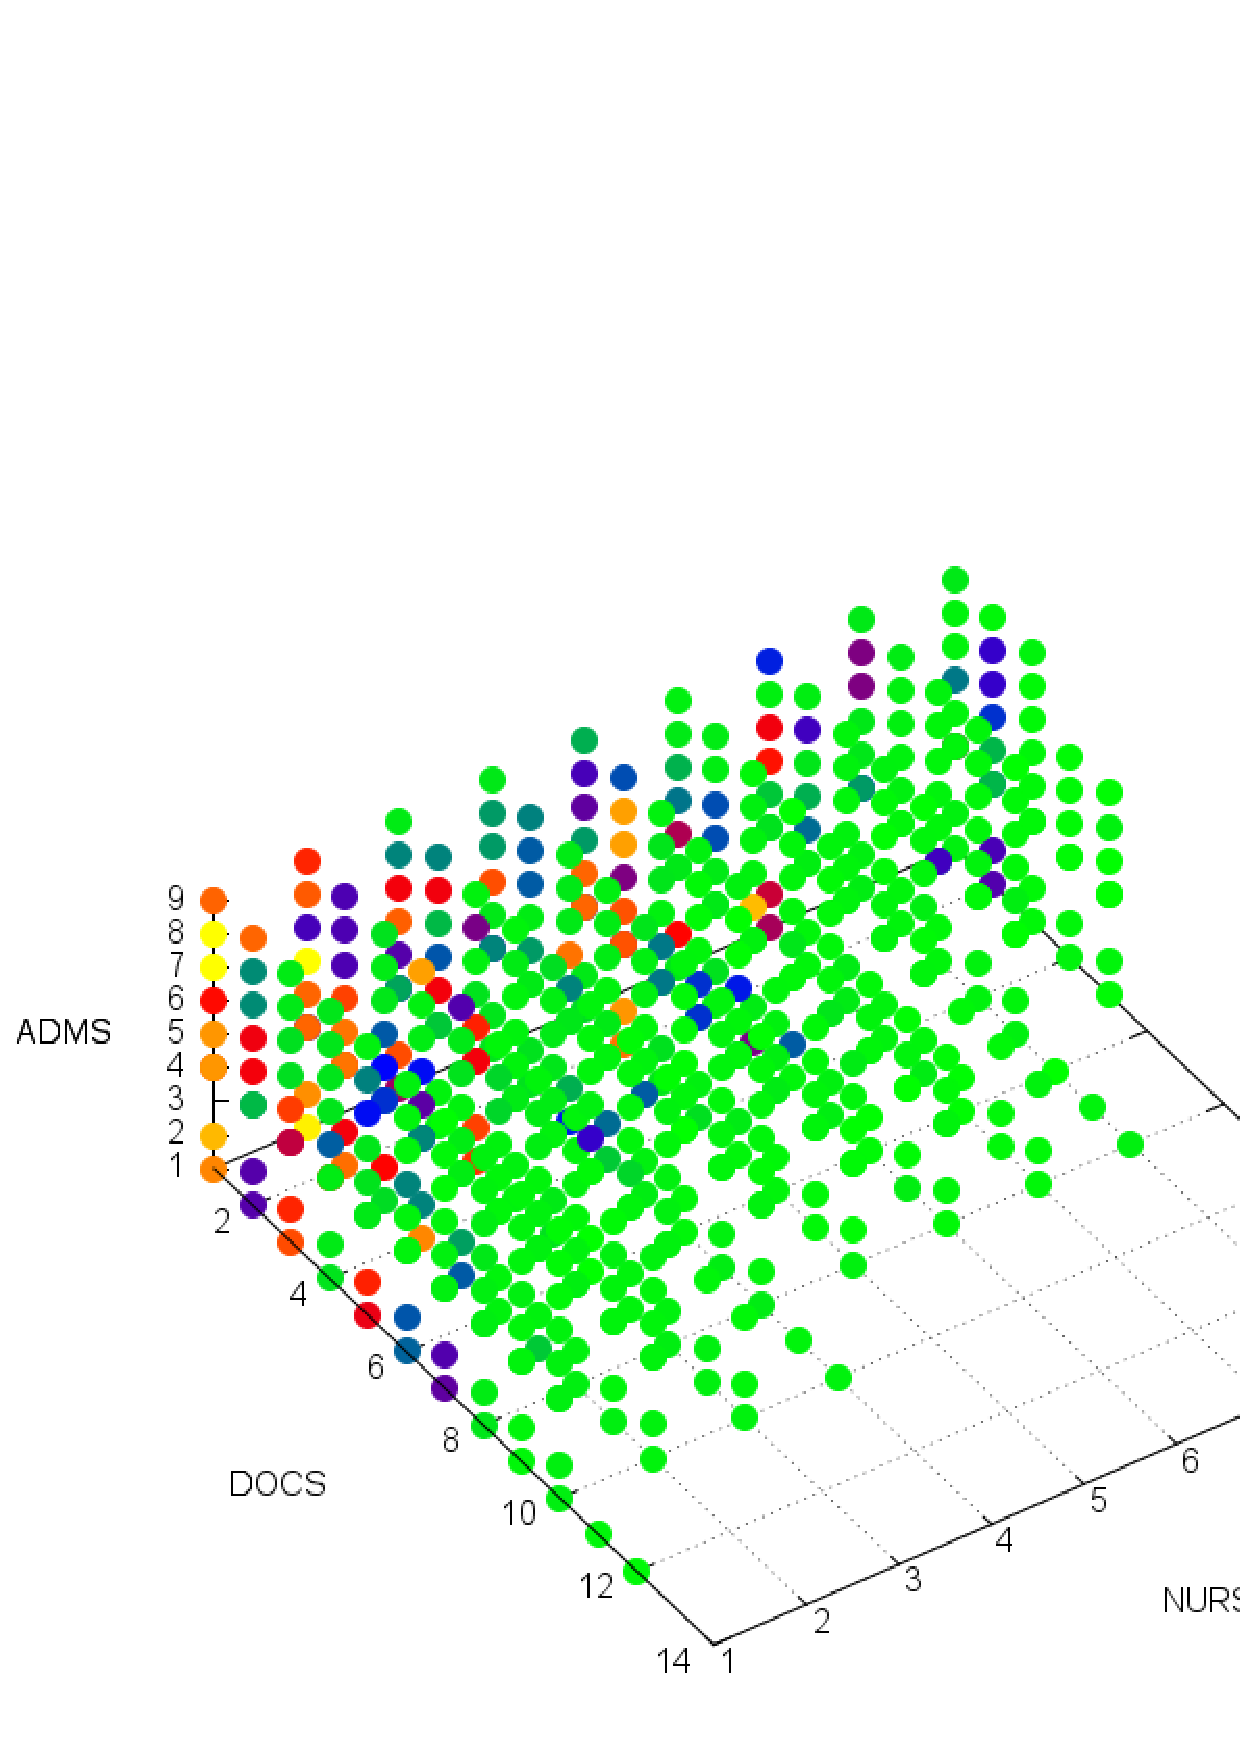
\includegraphics[width=0.88\columnwidth,height=0.2\paperheight]{figs4/3D-scatter-LoS-$2}
\par\end{centering}

\caption{3D scattered graph ordered by the cost of sanitary staff configuration.
The green values of interest were not so scattered, but not interconnected.\label{fig:3D-scattered-LoS-cost} }


\end{figure}



\section{Workloads}

In order to analyse the performance of the ED, the real average four
hundred incoming patients daily arrive to the ED of Sabadell hospital
was considered as follows. This real input was divided into four scenarios,
i.e., four different workload scenarios, up to: 4, 9, 13, and 17 incoming
patients hourly, as shown in \ref{tab:scenarios} (i.e., up to 96,
216, 312, and 408, respectively for 24hrs.).
\begin{figure}[H]
 %
\noindent \begin{centering}
\centering{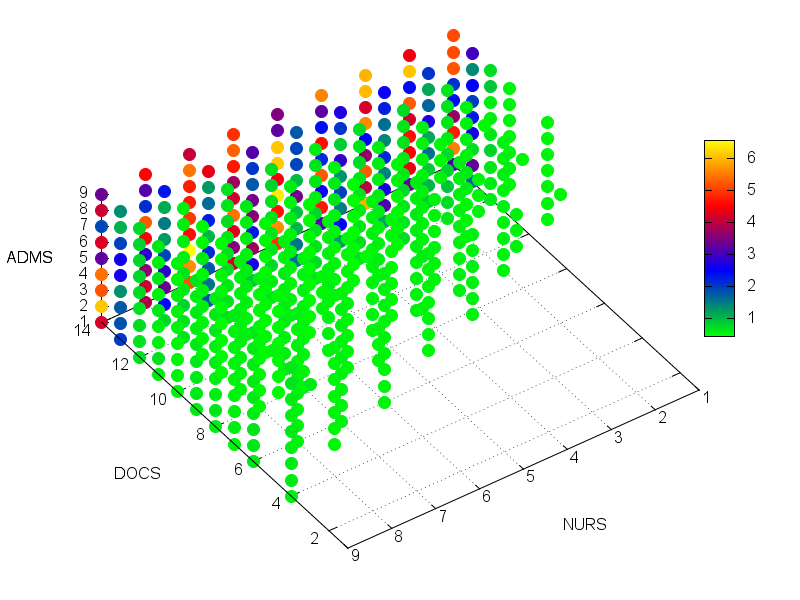
\includegraphics[width=0.88\columnwidth,height=0.2\paperheight]{figs4/3D-scatter-LoS-tpipe2}}
\par\end{centering}

  %
\caption{3D scattered graph ordered by the equivalent operational patient-service
time ({\bf t$^*$}) of a ``single one'' sanitary
professional of each sanitary staff configuration \ref{subtab:As-pipe}
to \ref{subtab:XRs-pipe}. The green value region of interest was
connected and almost ``non'' scattered.\label{fig:3D-scattered-LoS-tpipe} }
\end{figure}
 These different workload scenarios were used to supply different
loads to the ED, whereas the percentage of the priority level of patients
was maintained. 

\begin{table}[H]
\centering{}\caption{Incoming ED patients divided into four different workload scenarios,
up to: 4, 9, 13, and 17 patients per hour for each scenario. \label{tab:scenarios}}
\resizebox{2.3in}{!}{ %
\begin{tabular}{>{\centering}m{3.7cm}>{\centering}m{3.75cm}}
\hline 
Workload scenario number & \textbf{Incoming patients (hourly)} \tabularnewline
\hline 
1 & 4\tabularnewline
2 & 9\tabularnewline
3 & 13\tabularnewline
4 & 17\tabularnewline
\hline 
\end{tabular}}
\end{table}
\clearpage{}


\section{Evaluation Metrics}

The set of metrics used in this work were: the length of stay (LoS)
of the patients in the ED; the number of attended patients per day
(Throughput); and a compound index, the product of the cost of a given
sanitary staff configuration times patient length of stay (CLoS).

Furthermore, the computing time of each of the proposed optimisation
method is measured in order to observe the gains in reducing computing
time of the methodology proposed.\\


All simulations of the ED optimization cases analysed in this work
were carried out in a Linux cluster of the CAOS Department of the
UAB, which has 608 computing cores and 2.2TB of RAM, that is composed
of: 9 nodes of a dual-4 core Intel Xeon E5430, 2.6GHz, 16GB RAM; 1
node of 2xdual-6 core Intel Xeon E5645, 2.4GHz, 24GB RAM; and 8 nodes
of 4x16-cores AMD Opteron ``Interlagos'', 1.66GHz, 256 GB RAM, all
in a switched 1GigE network.


\section{Evaluation Method}

The evaluation of the proposed methodology was aimed to confirm the
correct operation of both the pipeline approach (PA) and the MC plus
the K-means methods, described in \ref{chap3:Math}. To this end,
we have first performed the exhaustive search (ES) to use as baseline
method. The second step of this evaluation consists on applying the
coarse grained phase, using either the PA, the MC plus K-means methods,
or both. Finally, the fine grained phase is apply in the promising
regions found in the previous step. 

In order to evaluate quantitatively the proposal methodology two case
studies were set. The first of them, namely case study A, was performed
using the agent-based ED simulator version 1.1. This case study is
further described in \ref{sub:Case-Study-A}. The second case or case
study B was performed using the agent-based ED simulator version 1.2
(the current version). This case study is further described in \ref{sub:Case-Study-B}.

In both case studies, only patients identified as triage level 4 and
5 are served at the stage of diagnosis-treatment phase, the three
metrics, and the four different workloads stated above were tested,
and the period simulated was 24 hrs., i.e., one day of functioning
of the ED, in all the experiments. Test scenarios and evaluation results
of both case studies are explained in detail in the following sections.\\


It is important to remind that the actions and interactions corresponding
to the admission and triage processes have been totally implemented,
but in the case of diagnostic and treatment phase, respecting to the
priorities of the Sabadell Hospital ED currently only the level 1
was implemented. In such level 1 only patients identified with priority
level 4 or 5 (less urgent, and non-urgent, respectively \ref{sec:active-agents})
were taken care of. Nevertheless, all incoming patients were triaged.
Once patients have been triaged, only patients identified as triage
level 4 and 5 were served at the stage of diagnosis-treatment phase.

\begin{comment}
In order to ensure the statistical value of the experiments performed,
it was necessary to execute multiple instances of the simulation with
varying random number seeds. As a rule of thumb, between two to three
tens of runs of a simulation with different random number seeds should
provide enough data to build a useful confidence interval around the
simulation results \cite{Stevens:1986}. Therefore, the simulation
model should be evaluated several times using different random seeds,
and the results obtained in such individuals simulations should be
combined in some way, v.gr., by using their average values, in order
to estimate a typical behaviour of the system. Thus, it avoids erroneous
and inaccurate analysis of the results allowing a greater degree of
confidence. 

The following two case studies presented have been conducted taking
into account the above stated issues for statistical validity. Evaluation
results and test scenarios of both case studies are explained in detail
in the following subsections.
\end{comment}



\section{Case Study A \label{sub:Case-Study-A}}

The agent-based ED simulator version 1.1, which is shown in \ref{fig:ED-SIM-0},
was used in this case study. In this version of the ED simulator the
diagnostic and treatment phase is only addressed by doctors. 
\begin{figure}[h]
\noindent \begin{centering}
\centering 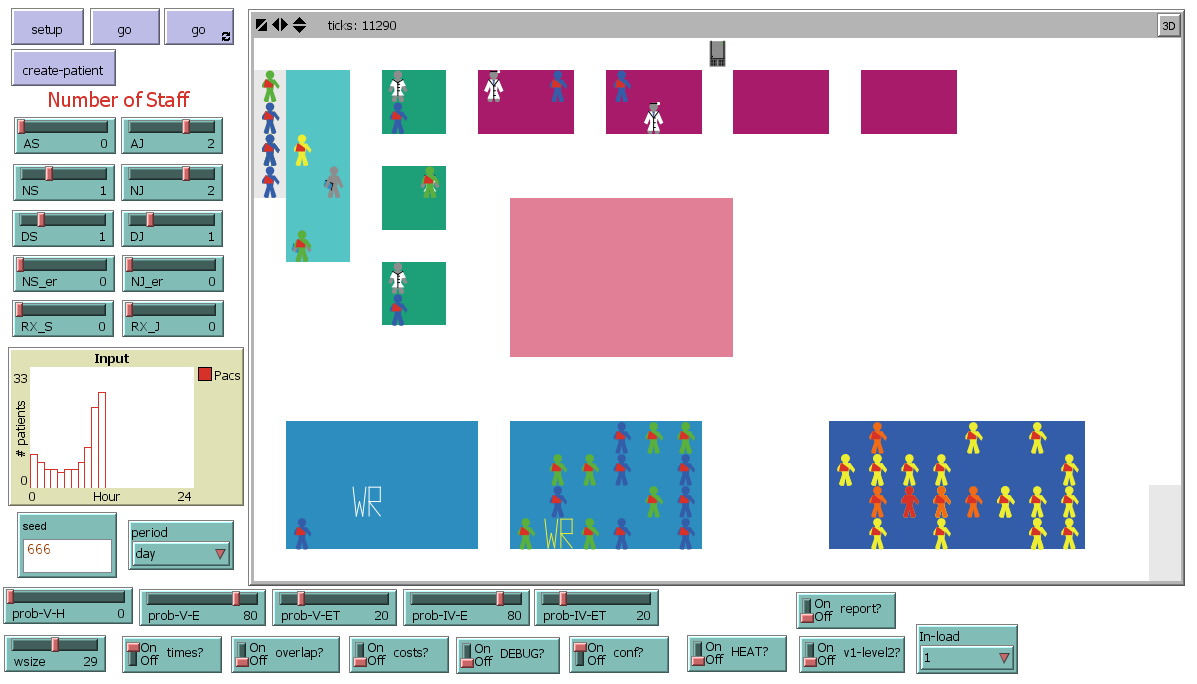
\includegraphics[width=0.9\columnwidth,height=0.16\paperheight]{figs2/ED_Netlogo-0}
\par\end{centering}

\noindent \caption{ED simulator v1.1. Admission personnel, triage nurses, and doctors
were the sanitary staff considered.}


\label{fig:ED-SIM-0} 
\end{figure}
 The simple patient flow in this ED simulator is defined as follows:
patients arrive to the ED on their own, and waits to be attended in
the admission area. Then, patients stay in the first Waiting Room
(WR) WR1, until a triage nurse call them. After the triage process
patients identified as triage level 4 and triage level 5 pass to a
second WR2, and stay there until a free doctor calls them to begin
the diagnosis-treatment phase, depending on the patient's symptoms,
physical condition, and prescribed diagnosis tests. Finally, patients
are discharged from the ED. 

Therefore, in this case study the sanitary staff considered were:
doctors, triage nurses, and admission personnel. Thus, only \ref{subtab:As}
to \ref{subtab:Ds} were taken into account. As a result, 1,134 ($14D*9N*9A$)
staff configurations were tested for each of the four workload scenarios
of incoming patients stated in \ref{tab:scenarios}. 

Finally, the three metrics above stated: LoS, Throughput, and CLoS
were obtained by applying: the ES technique; the coarse grained phase,
using both the PA and the MC plus K-means methods; then, the fine
grained phase was applied in the reduced feasible region to find the
optimum.

\begin{comment}
\begin{figure}[h]
\hfill{}%
\begin{minipage}[c]{0.45\columnwidth}%
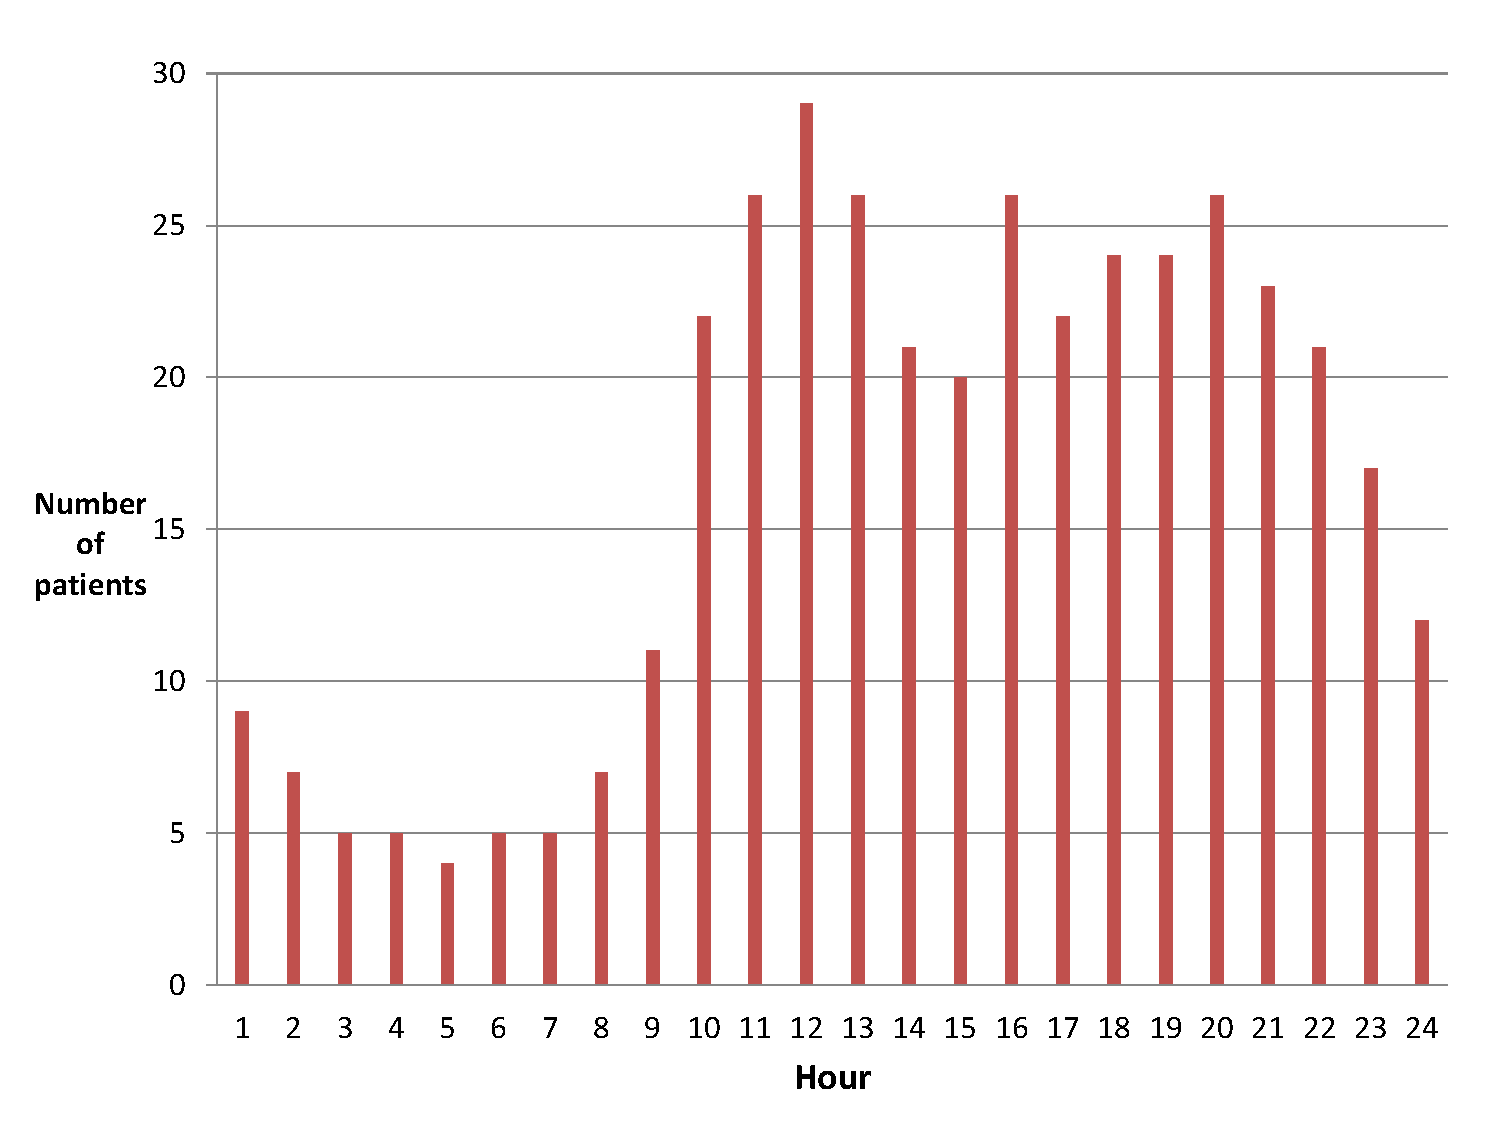
\includegraphics[width=1\columnwidth]{figs4/input.pdf}\caption{}
%
\end{minipage}\hfill{}%
\begin{minipage}[c]{0.45\columnwidth}%
\begin{center}
\resizebox{1.8in}{!}{ %
\begin{tabular}{>{\centering}m{1.5cm}>{\centering}m{1.75cm}}
\hline 
Scenario number & \textbf{Incoming patients (hourly)} \tabularnewline
\hline 
1 & 4\tabularnewline
\hline 
2 & 8\tabularnewline
\hline 
3 & 13\tabularnewline
\hline 
4 & 17\tabularnewline
\hline 
\end{tabular}}\caption{}

\par\end{center}%
\end{minipage}\hfill{}
\end{figure}
\end{comment}



\subsection{LoS Index}

The first objective set was to minimise patient length of stay (LoS)
in the ED, with cost configuration constraint less or equal to 3,500
euro. This first index is expressed mathematically in \ref{eq:LoS index}:
\begin{equation}
\begin{aligned} & {\text{minimise LoS}} &  & f(D,N,A)\\
 & \text{subject to} &  & D_{cost}+N_{cost}+A_{cost}\in Cost\leq3,500\:\text{euro}
\end{aligned}
\label{eq:LoS index}
\end{equation}


It is worth noting that each of the plotted points for the following
four workload scenarios were obtained running the ED simulator as
many times as points are. Each plotted point corresponds to each of
the 602 staff configurations (out of 1,134) that satisfy the cost
restriction.


\subsubsection{First Workload Scenario}

The results of this scenario, up to 4 patients/hour, are shown from
\ref{subfig:es4-1} to \ref{subfig:km4-1}. The ES result is shown
in \ref{subfig:es4-1}. The red triangle was the minimum. 
\begin{figure}[H]
\noindent \begin{centering}
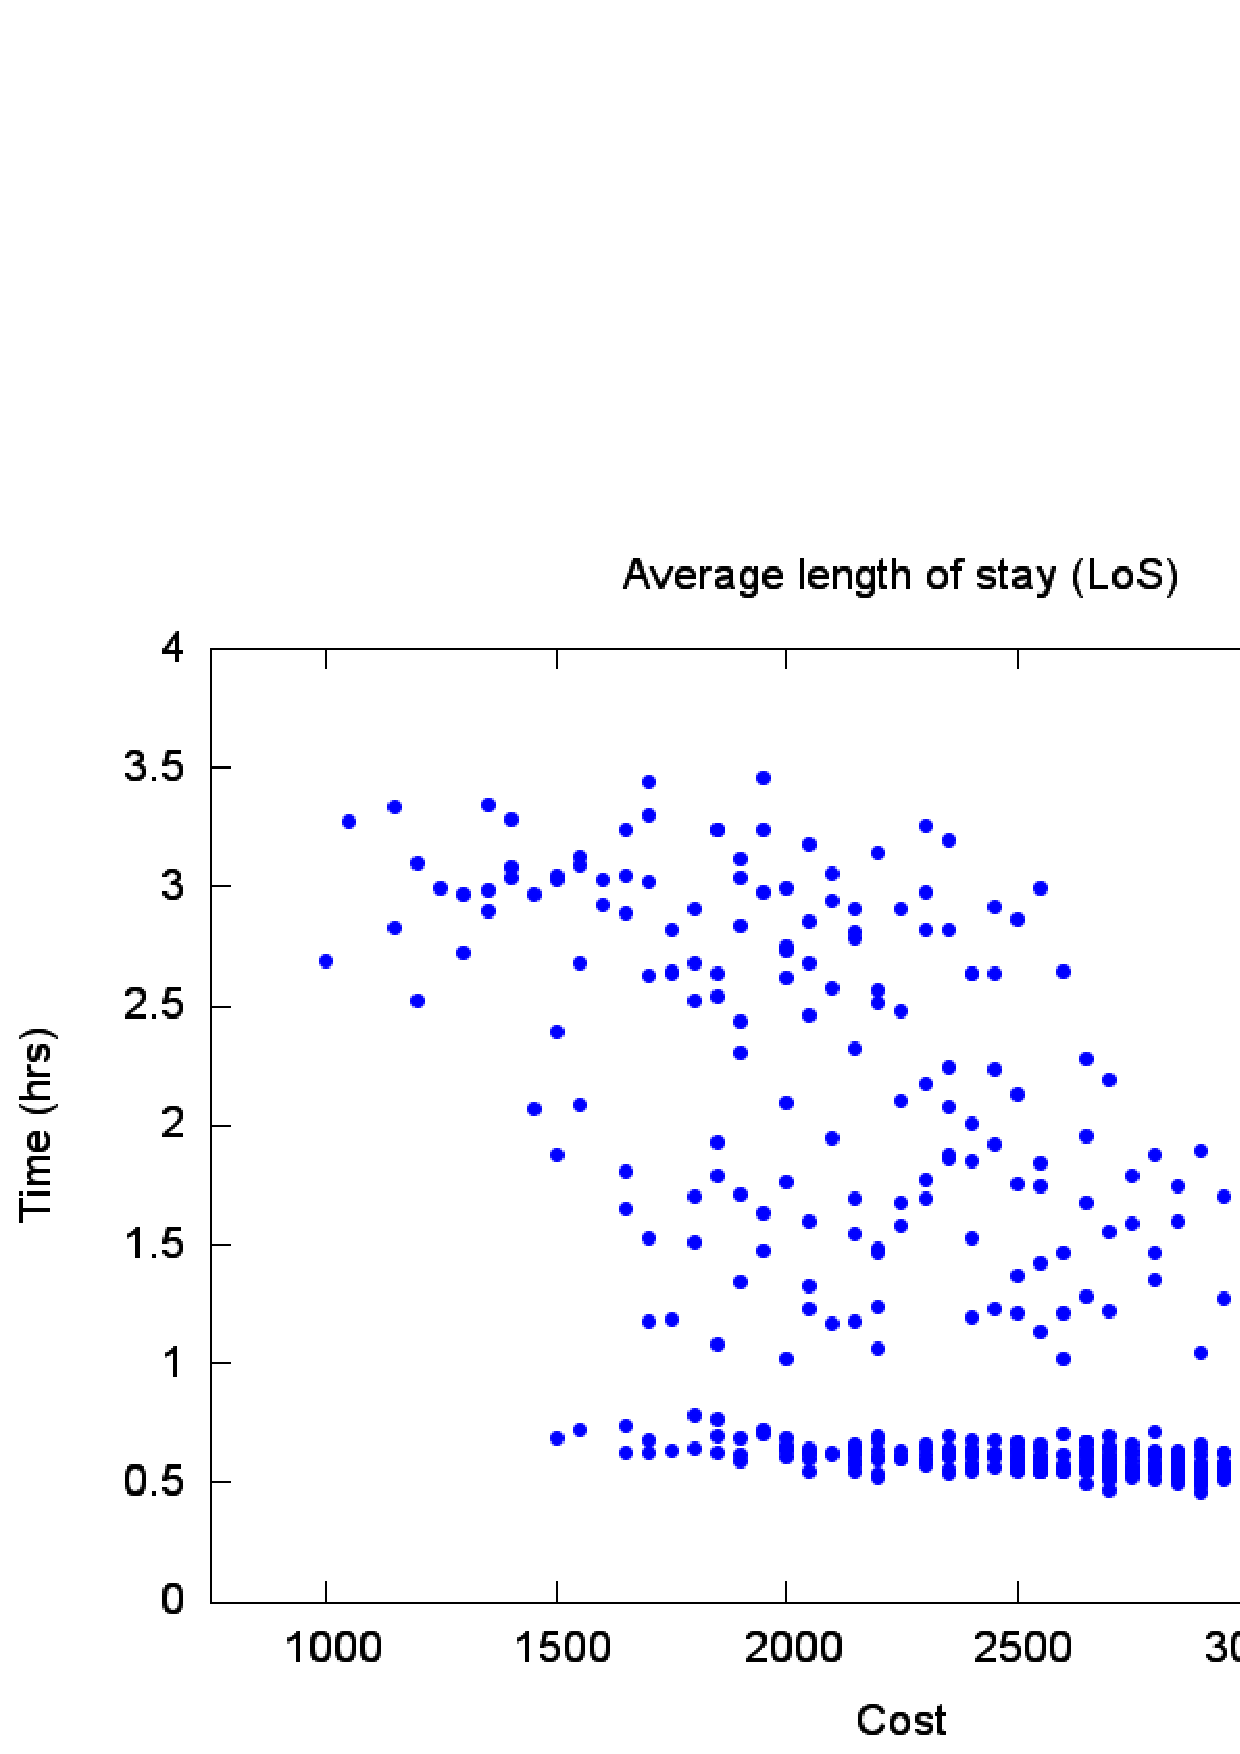
\includegraphics[width=0.95\columnwidth,height=0.23\paperheight]{figs4/v0/6400-602-25-exh-LoS-min}
\par\end{centering}

\caption{Average LoS obtained by the ES. The red triangle was the minimum.
\label{subfig:es4-1}}
\end{figure}


The PA result is shown in \ref{subfig:pipe4-1}, where four regions
can be clearly seen and the red triangle was the minimum. 
\begin{figure}[H]
\noindent \begin{centering}
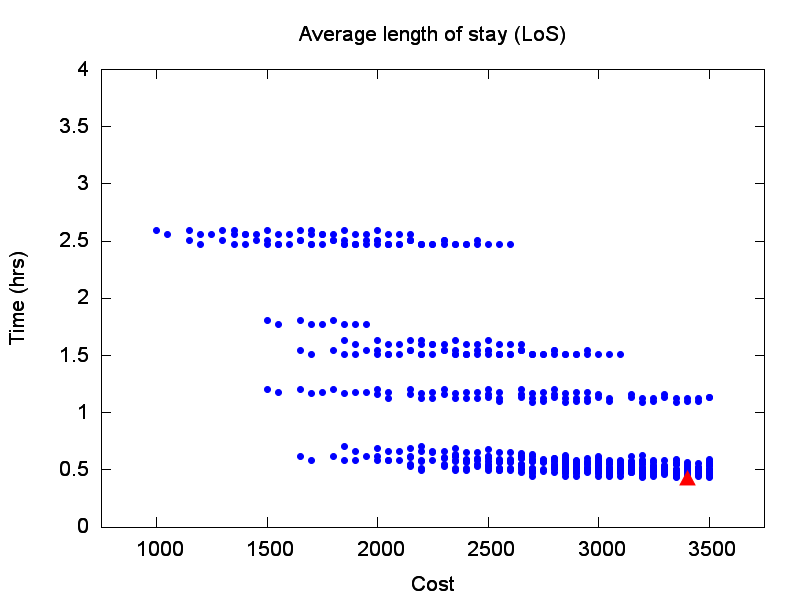
\includegraphics[width=0.95\columnwidth,height=0.23\paperheight]{figs4/v0/6400-602-25-pipe-LoS-min}
\par\end{centering}

\caption{Average LoS obtained by the PA. The red triangle was the minimum.
\label{subfig:pipe4-1}}
\end{figure}
The most important is the bottom region, in which the average minimum
LoS was around 0.5 hours. There were 366 configurations (from a total
of 602 in the feasible region) in this region, which is the one where
the minimum was.

The MC plus the K-means methods results are shown in \ref{subfig:mc4-1}
to \ref{subfig:km4-1}, respectively. The MC method found 75 configurations.
\begin{figure}[H]
\noindent \centering{}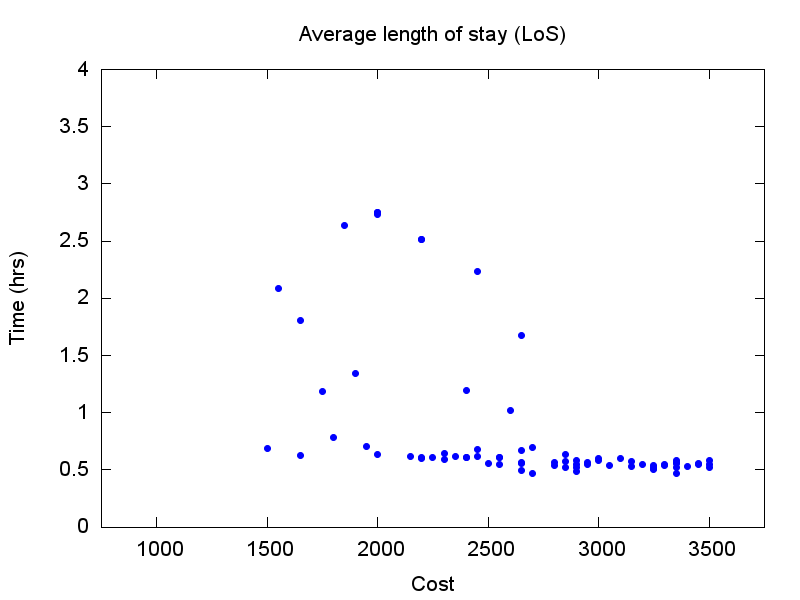
\includegraphics[width=0.95\columnwidth,height=0.23\paperheight]{figs4/v0/MC/MC-6400-602-25-69-25-75confs-LoS}\caption{Average LoS of 75 configurations obtained by the MC method. \label{subfig:mc4-1}}
\end{figure}
 However, it was difficult to get any conclusion about such region;
therefore, the complementary K-means method was performed. The K-means
method identified three different clusters, shown in \ref{subfig:km4-1}.
The most important cluster was the red one (at the bottom right),
which delimited the region where the optimum was. 
\begin{figure}[H]
\noindent \centering{}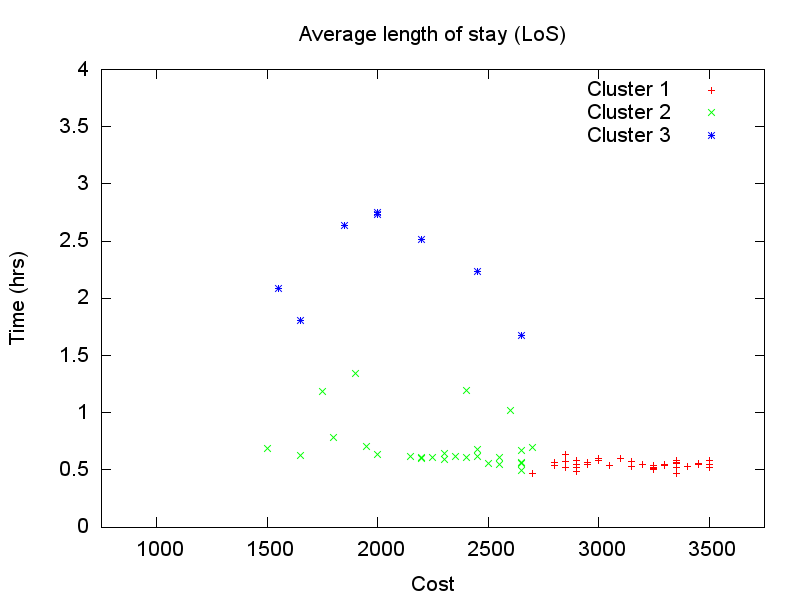
\includegraphics[width=0.95\columnwidth,height=0.23\paperheight]{figs4/v0/MC/K-means-6400-602-25-69-25-75-Cluster1-36_Cluster2-27_Cluster3-8}\caption{K-means identified three clusters of average LoS . The red one delimits
the region where the minimum was.\label{subfig:km4-1}}
\end{figure}
 %
\begin{comment}
but the green cluster was also important, because the average LoS
of such configurations were not so different from the red cluster.
\end{comment}


The \ref{fig:3D-scattered-graph-25} shows another way to visualise
the connectivity characteristic of the reduced regions found by the
proposed methodology. The axes of such graph are the equivalent operational
patient-service time ({\bf t$^*$}) of a ``single
one'' sanitary professional of each sanitary staff configuration
(the first column of \ref{subtab:As-pipe} to \ref{subtab:Ds-pipe},
where they were ordered by the PA \ref{eq:Pipeline formula}). In
such figure, the points of interest were the green points, which lie
in the region of interest, where the minimum was, which can be seen
in black triangle. It can be seen that it was not necessary to search
in the whole feasible region, but only in the green connected region. 

\begin{figure}[h]
\noindent \begin{centering}
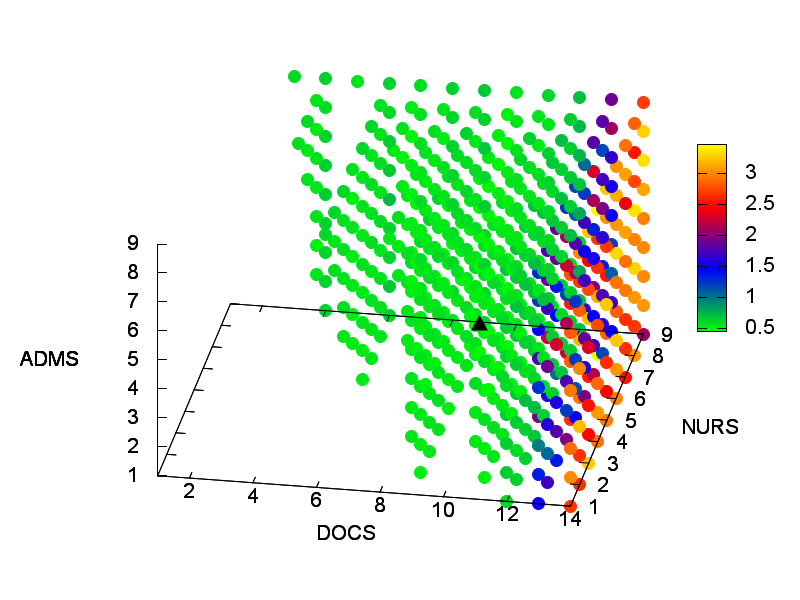
\includegraphics[width=0.95\columnwidth,height=0.2\paperheight]{figs4/v0/6400-602-25-3D-scatter-LoS2}
\par\end{centering}

\caption{3D scattered graph shows the average LoS index of the first workload
scenario (4 patients/hour). The average LoS index in hours is represented
in colour, and the minimum is the black triangle.\label{fig:3D-scattered-graph-25} }
\end{figure}


Finally, after separately applied both the PA and the MC plus the
K-means methods, the \textquotedblleft{}reduced exhaustive search\textquotedblright{}
was separately performed in each reduced region identified. The optimum
found per each method: the ES, the PA, and the MC plus the K-means
methods are presented in \ref{tab:4p-a}, where the sanitary staff
configuration (doctors, nurses, and admission personnel), their associated
average minimum LoS, and cost configuration are shown. The three optima
independently found were the same. 

\begin{comment}
\begin{figure}[H]
\noindent \begin{centering}
\begin{minipage}[t][1\totalheight][s]{0.95\columnwidth}%
\noindent \begin{center}
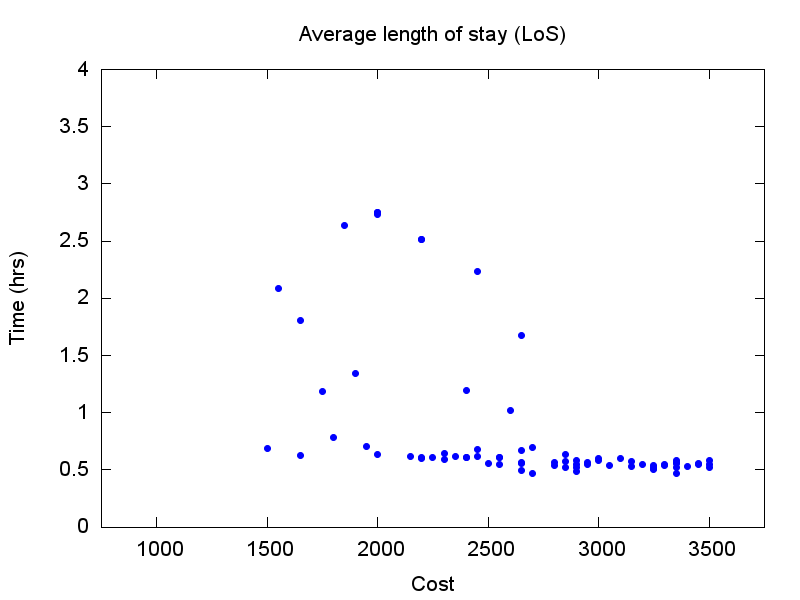
\includegraphics[width=0.95\columnwidth,height=0.25\paperheight]{figs4/v0/MC/MC-6400-602-25-69-25-75confs-LoS.png}
\par\end{center}

\vspace*{-1cm}

\noindent \begin{center}
\caption{Average LoS of 75 configurations obtained by the MC method. }

\par\end{center}%
\end{minipage}
\par\end{centering}

\noindent \begin{centering}
\vspace{0cm}
\vspace*{-1.2cm}
\par\end{centering}

\noindent \begin{centering}
\begin{minipage}[t][1\totalheight][s]{0.95\columnwidth}%
\noindent \begin{center}
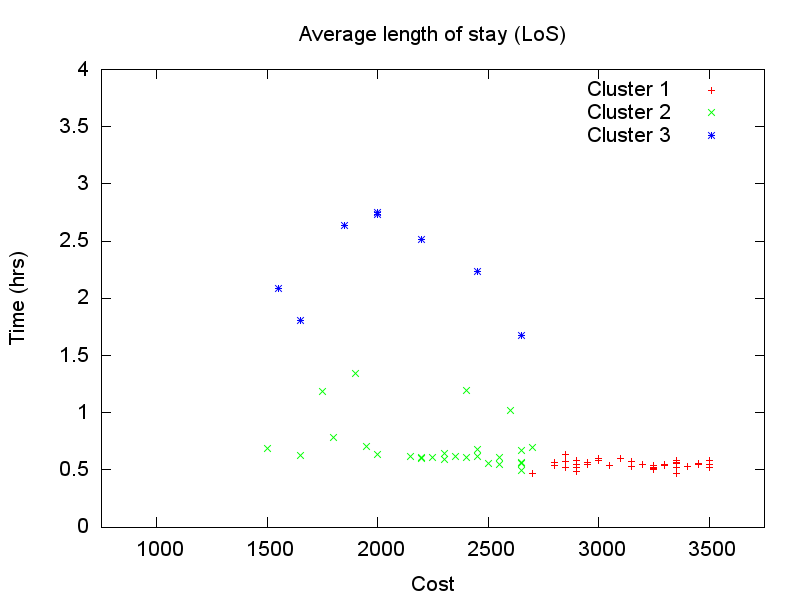
\includegraphics[width=0.95\columnwidth,height=0.25\paperheight]{figs4/v0/MC/K-means-6400-602-25-69-25-75-Cluster1-36_Cluster2-27_Cluster3-8.png}\vspace*{-0.8cm}
\par\end{center}

\caption{K-means identified three clusters of average LoS . The red one delimits
the region where the minimum is.}
%
\end{minipage}
\par\end{centering}

%\vspace*{0.4cm}%{\bf Figures} show the average LoS index of the first workload scenario (4 patients/hour) using the ES, the PA, and the MC+K-means methods.
\end{figure}
\end{comment}
%\vspace*{-.2cm}%
\begin{comment}
 \begin{figure}[htb!]  
\centering 
\begin{tabular}{cc}         
	\subfloat[][Average patient LOS with P = 20\%]{                 		\includegraphics[width=75mm,height=60mm]{figs4/v0/6400-602-25-pacs-totales-sort-pipe-meantime-exh-min-CINCO.pdf} 
		\label{subfloat:exp1_20} 
	} 
&        
	\subfloat[][Average patient LOS with P = 40\%]{                 		\includegraphics[width=75mm,height=60mm]{figs4/v0/pipe-sorted-LoS\_0-2\5_min.pdf}                 		\label{subfloat:exp1_40}        
} 
\\ 	
	\subfloat[][Average patient LOS with P = 20\%]{                 		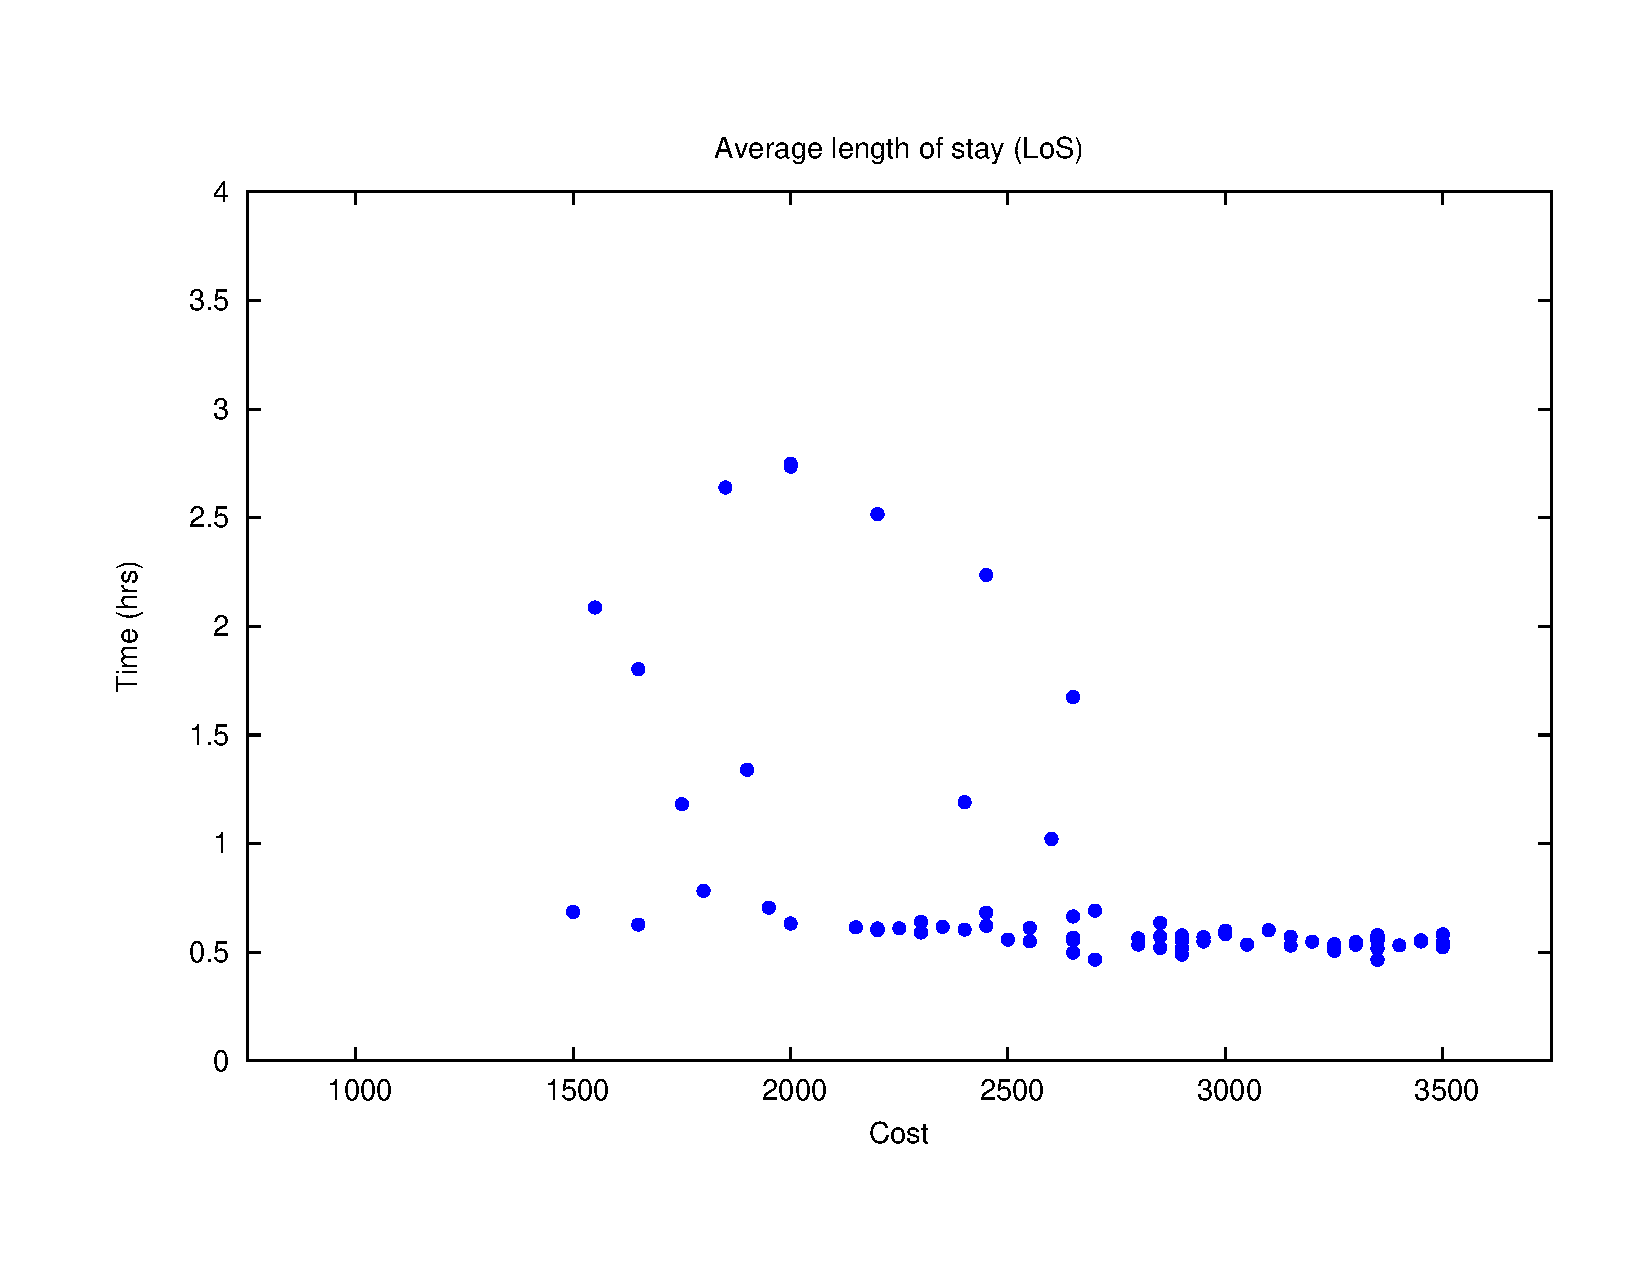
\includegraphics[width=75mm,height=60mm]{figs4/v0/MC/MC-6400-602-25-69-25-75confs-LoS-TRI.pdf} 
		\label{subfloat:exp1_20} 
	} 
& 
 \subfloat[][Average patient LOS with P = 40\%]{                 		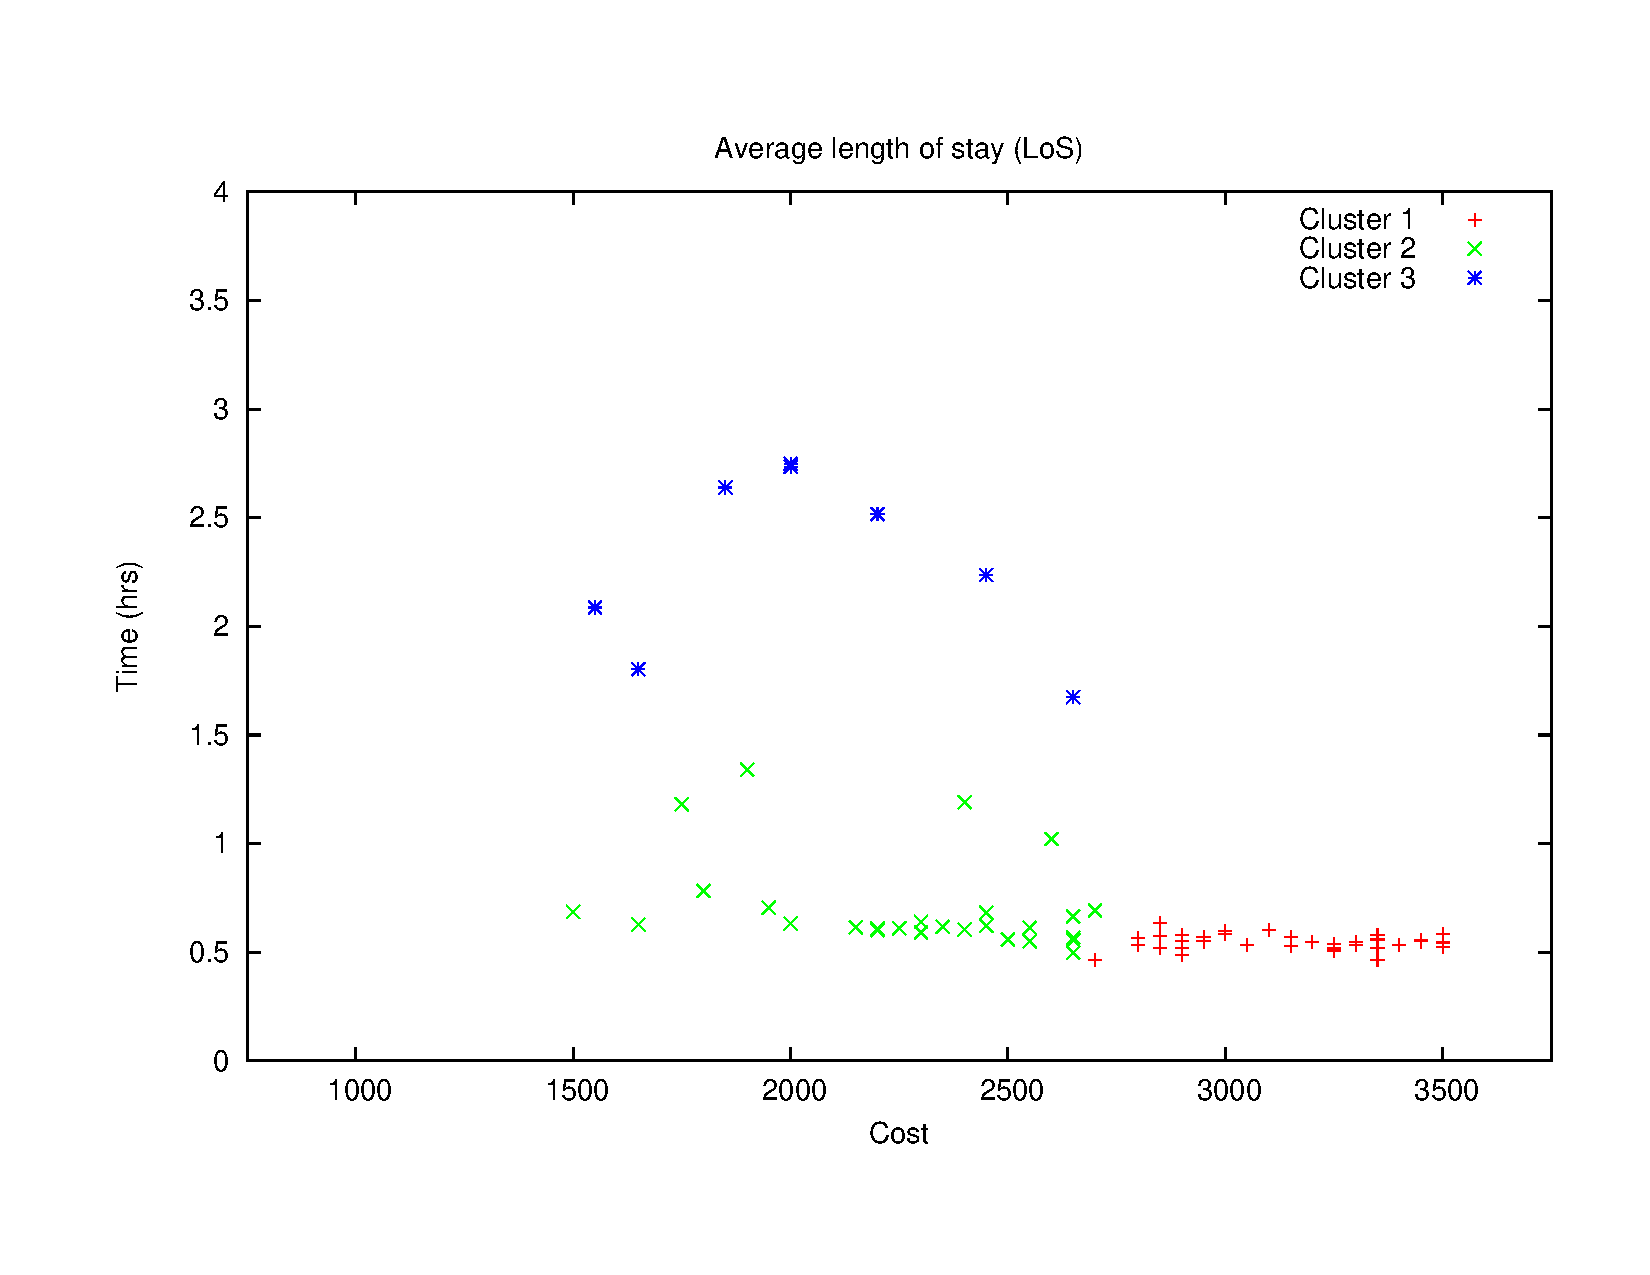
\includegraphics[width=75mm,height=60mm]{figs4/v0/MC/K-means-6400-602-25-69-25-75-Cluster1-36_Cluster2-27_Cluster3-8_TRI.pdf}                 		
		\label{subfloat:exp1_40}        
} 
\end{tabular}
\caption{Average patient LOS. Red and green points are the minimum.} 
\label{fig:exp1_20_40} 
\end{figure} 
\end{comment}
\begin{comment}
\begin{figure}[H]
\noindent \begin{centering}
\begin{minipage}[t][1\totalheight][s]{0.49\columnwidth}%
\noindent \begin{center}
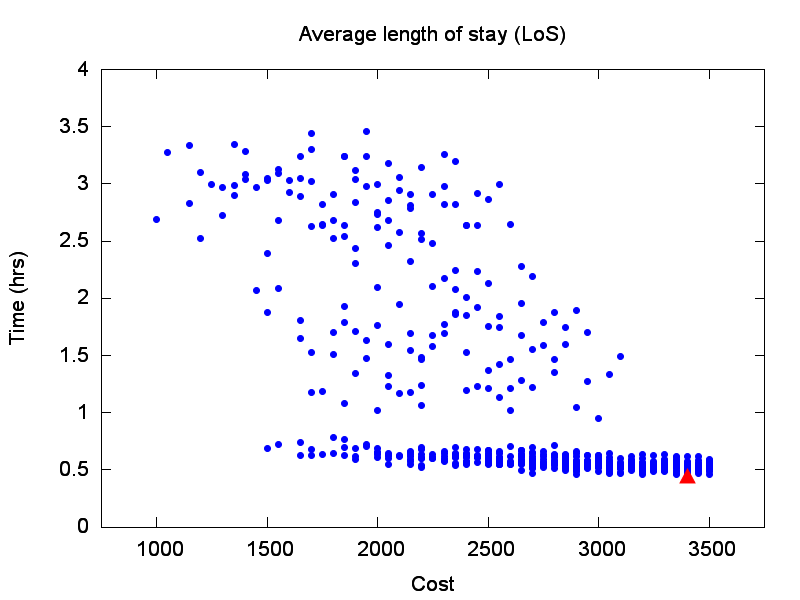
\includegraphics[width=1\columnwidth]{figs4/v0/6400-602-25-exh-LoS-min.png}
\par\end{center}

\vspace*{-1cm}

\noindent \begin{center}
\caption{Average LoS obtained by the ES method. The red triangle was the minimum.
\label{subfig:es4}}

\par\end{center}%
\end{minipage}\hfill{}%
\begin{minipage}[t][1\totalheight][s]{0.49\columnwidth}%
\noindent \begin{center}
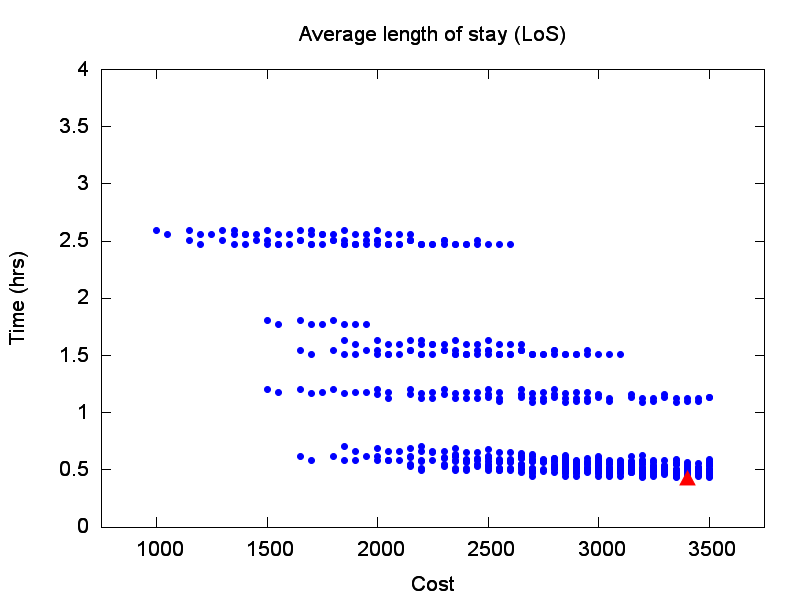
\includegraphics[width=1\columnwidth]{figs4/v0/6400-602-25-pipe-LoS-min.png}
\par\end{center}

\vspace*{-1cm}

\noindent \begin{center}
\caption{Average LoS obtained by the PA. The red triangle is the minimum. \label{subfig:pipe4}}

\par\end{center}%
\end{minipage}
\par\end{centering}

\noindent \begin{centering}
%\centering\vspace{0cm}
\vspace*{-1.2cm}
\par\end{centering}

\begin{minipage}[t][1\totalheight][s]{0.49\columnwidth}%
\noindent \begin{center}
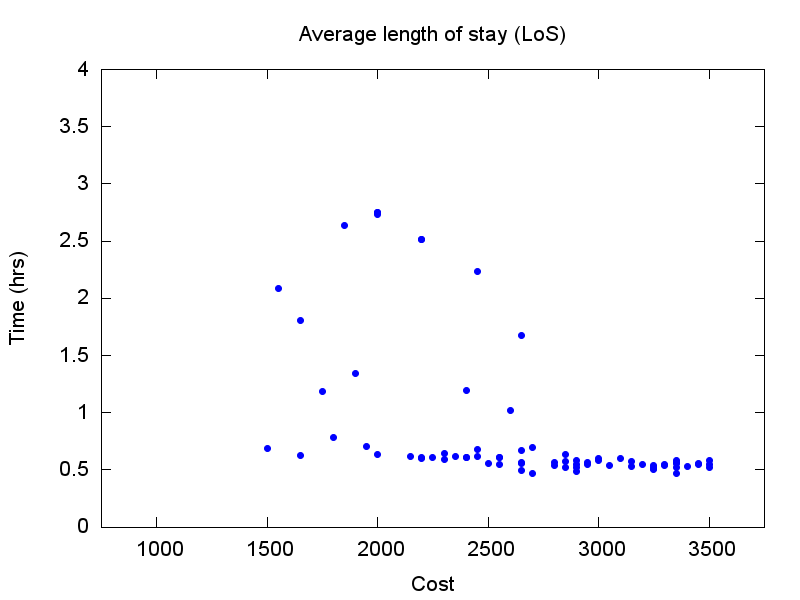
\includegraphics[width=1\columnwidth]{figs4/v0/MC/MC-6400-602-25-69-25-75confs-LoS.png}\vspace*{-0.8cm}
\par\end{center}

\caption{Average LoS of 75 configurations obtained by the MC method. \label{subfig:mc4}}
%
\end{minipage}\hfill{}%
\begin{minipage}[t][1\totalheight][s]{0.49\columnwidth}%
\noindent \begin{center}
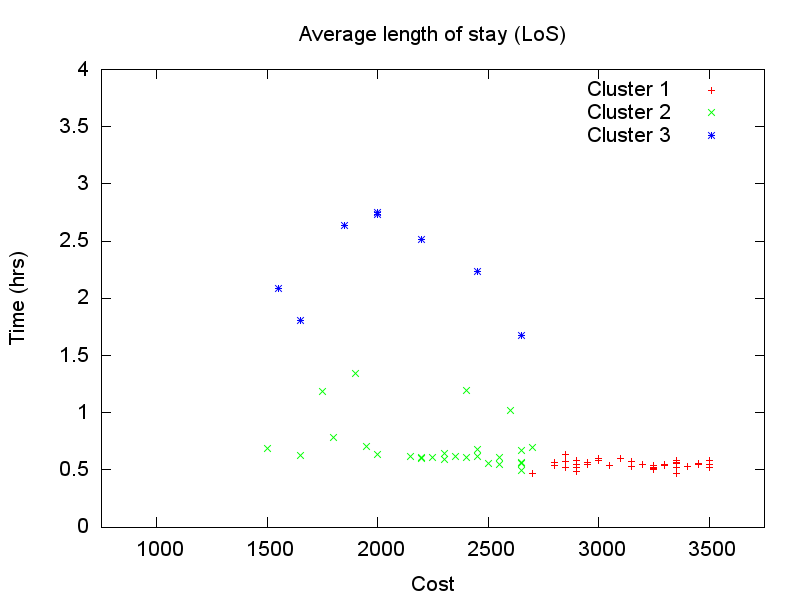
\includegraphics[width=1\columnwidth]{figs4/v0/MC/K-means-6400-602-25-69-25-75-Cluster1-36_Cluster2-27_Cluster3-8.png}\vspace*{-0.8cm}
\par\end{center}

\caption{The K-means method identified three clusters of average LoS. The red
one delimited the region where the minimum was.\label{subfig:km4}}
%
\end{minipage}

\vspace*{0.4cm}{\bf Figures} show the average LoS index of the first workload scenario (4 patients/hour) using the ES, the PA, and the MC+K-means methods.
\end{figure}
\end{comment}
\begin{comment}
\begin{figure}[H]
\hfill{}\subfloat[\label{subfloat:pipe4} Scattered 3D graph of doctors, nurses, and
admission personnel.]{

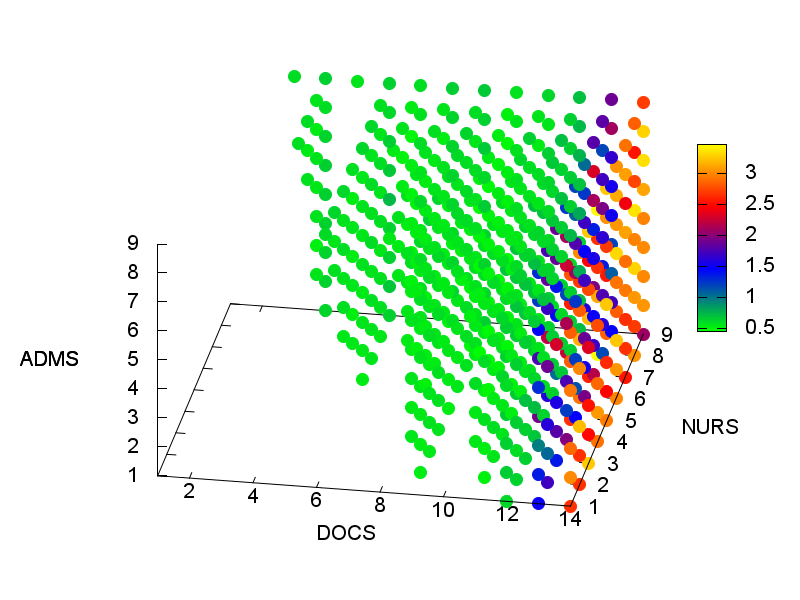
\includegraphics[width=0.48\columnwidth]{figs4/6400-602-25-3D-scatter-LoS.png}}\hfill{}\subfloat[\label{subfloat:contour4} Contour graph where doctors and nurses
can be seen.]{

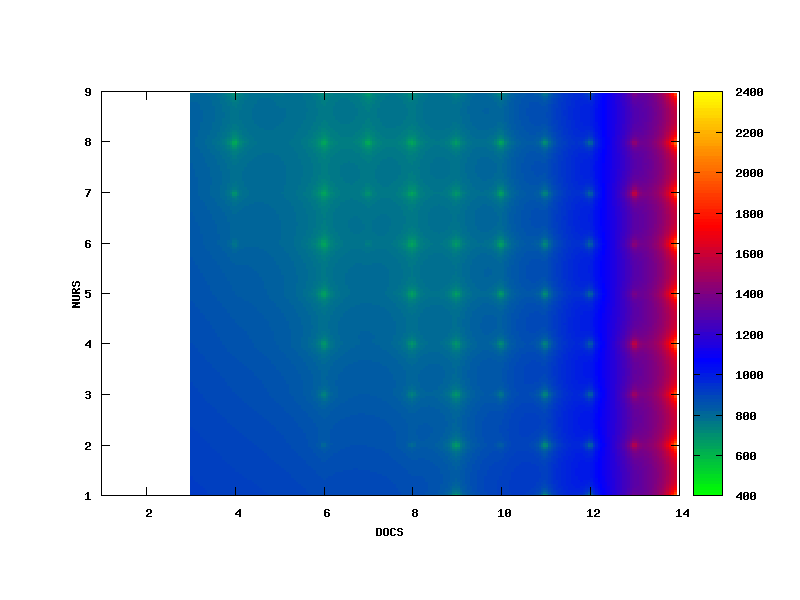
\includegraphics[width=0.48\columnwidth]{figs4/6400-602-25-sort-pipe_p5_y_p4-contour.png}}\hfill{}

\caption{\label{fig:Two-vision} Graphs show the average LoS index of the first
workload scenario (4 patients/hour) using the first column of \ref{subtab:As-pipe},
\ref{subtab:Ns-pipe}, and \ref{subtab:Ds-pipe}, where they were
ordered by the pipeline approach (PA) \ref{eq:Pipeline formula}.
The colour bar is expresed in tics ( $hours\:=\frac{tics}{1000}$
).}
\end{figure}
\end{comment}
\begin{comment}
\begin{figure}[H]
\noindent \begin{centering}
\begin{minipage}[t][1\totalheight][s]{1\columnwidth}%
 %
\noindent \begin{center}
\centering{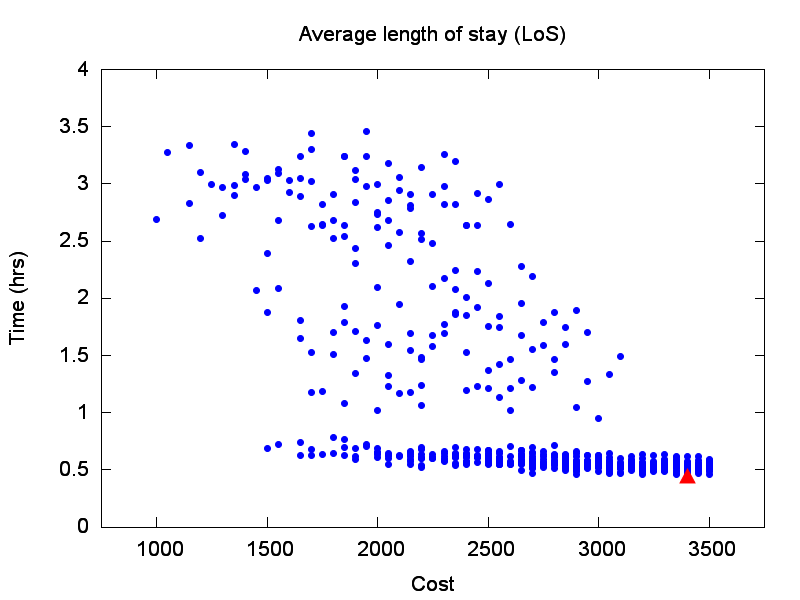
\includegraphics[scale=0.4]{figs4/v0/6400-602-25-exh-LoS-min.png}}
\par\end{center}

  %
\vspace*{-1cm}

\noindent \begin{center}
\caption{Average LoS obtained by the ES method, the red triangle is the minimum. }

\par\end{center}%
\end{minipage}
\par\end{centering}

\noindent \begin{centering}
%\centering\vspace{0cm}
\vspace*{-1.2cm}
\par\end{centering}

\noindent \begin{centering}
\begin{minipage}[t][1\totalheight][s]{1\columnwidth}%
\noindent \begin{center}
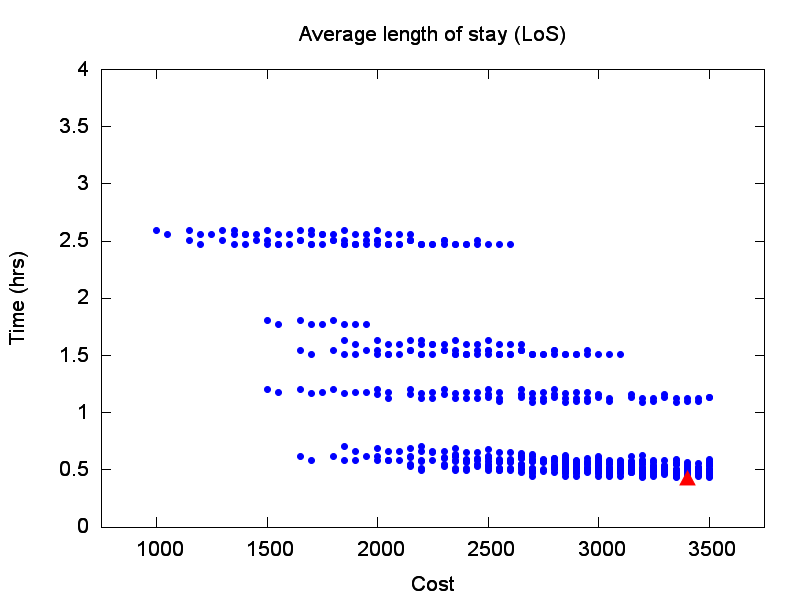
\includegraphics[scale=0.4]{figs4/v0/6400-602-25-pipe-LoS-min.png}\vspace*{-0.8cm}
\par\end{center}

\caption{Average LoS obtained by the PA, the red triangle is the minimum. }
%
\end{minipage}
\par\end{centering}

\noindent %\vspace*{0.4cm}%{\bf Figures} show the average LoS index of the first workload scenario (4 patients/hour) using the ES, the PA, and the MC+K-means methods.
\end{figure}
\end{comment}


\begin{table}[H]
\caption{Optimum staff configurations that got the average minimum LoS for
this workload scenario (up to 4 patients hourly), where S is Senior
and J is Junior. This optimum sanitary staff configuration is shown
in red triangle in \ref{subfig:es4-1} and in black triangle in \ref{fig:3D-scattered-graph-25}.}


\centering{}%
\begin{tabular}{cccccc>{\centering}p{2.8cm}}
\hline 
Method & euro & LoS (hrs) & D & N & A & Run time (hrs)

4 Pthreads\tabularnewline
\hline 
ES & 3,400  & 0.44 & 2S  & 2S & 2S & 0.89\tabularnewline
PA & 3,400 & 0.43 & 2S & 2S & 2S & 0.53\tabularnewline
MC+K-means & 3,400  & 0.44 & 2S  & 2S & 2S & 0.76\tabularnewline
\hline 
\end{tabular}\label{tab:4p-a} 
\end{table}


\begin{comment}
From Figures \ref{fig:exp1_20} and \ref{tab:4p-a}, there is a staff
configuration that got the minimum time. Also, in such Figures \ref{fig:exp1_20}
can appreciate that there are many other staff configurations that
are quite close to the optimum, but with less cost.
\end{comment}



\subsubsection{Second Workload Scenario}

The results of this scenario, up to 9 patients/hour, are shown from
\ref{subfig:es8-1} to \ref{subfig:km8-1}. The ES result is shown
in \ref{subfig:es8-1}, where the red triangle was the minimum. 
\begin{figure}[H]
\noindent \begin{centering}
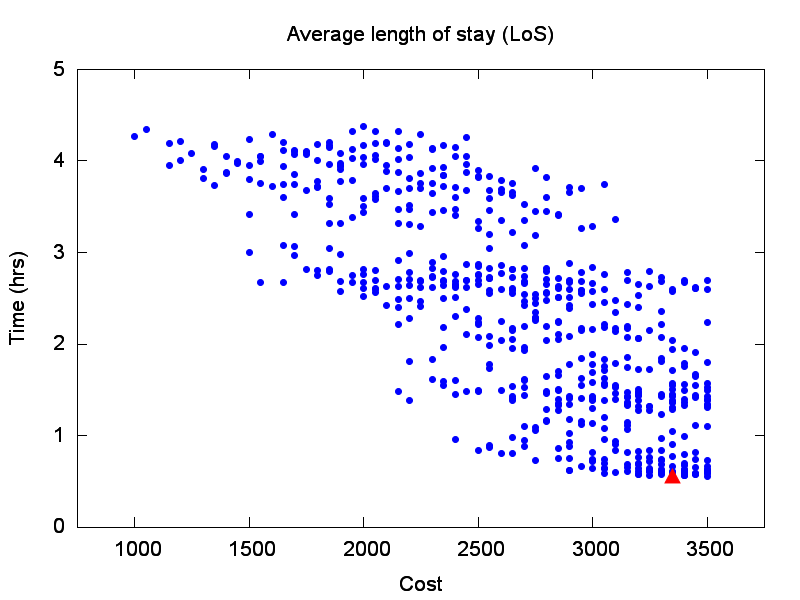
\includegraphics[width=0.95\columnwidth,height=0.25\paperheight]{figs4/v0/6400-602-50-exh-LoS-min}
\par\end{centering}

\caption{Average LoS obtained by the ES. The red triangle was the minimum.
\label{subfig:es8-1}}
\end{figure}


The PA result is shown in \ref{subfig:pipe8-1}, where seven regions
can be clearly seen and the red triangle is the minimum.
\begin{figure}[H]
\noindent \begin{centering}
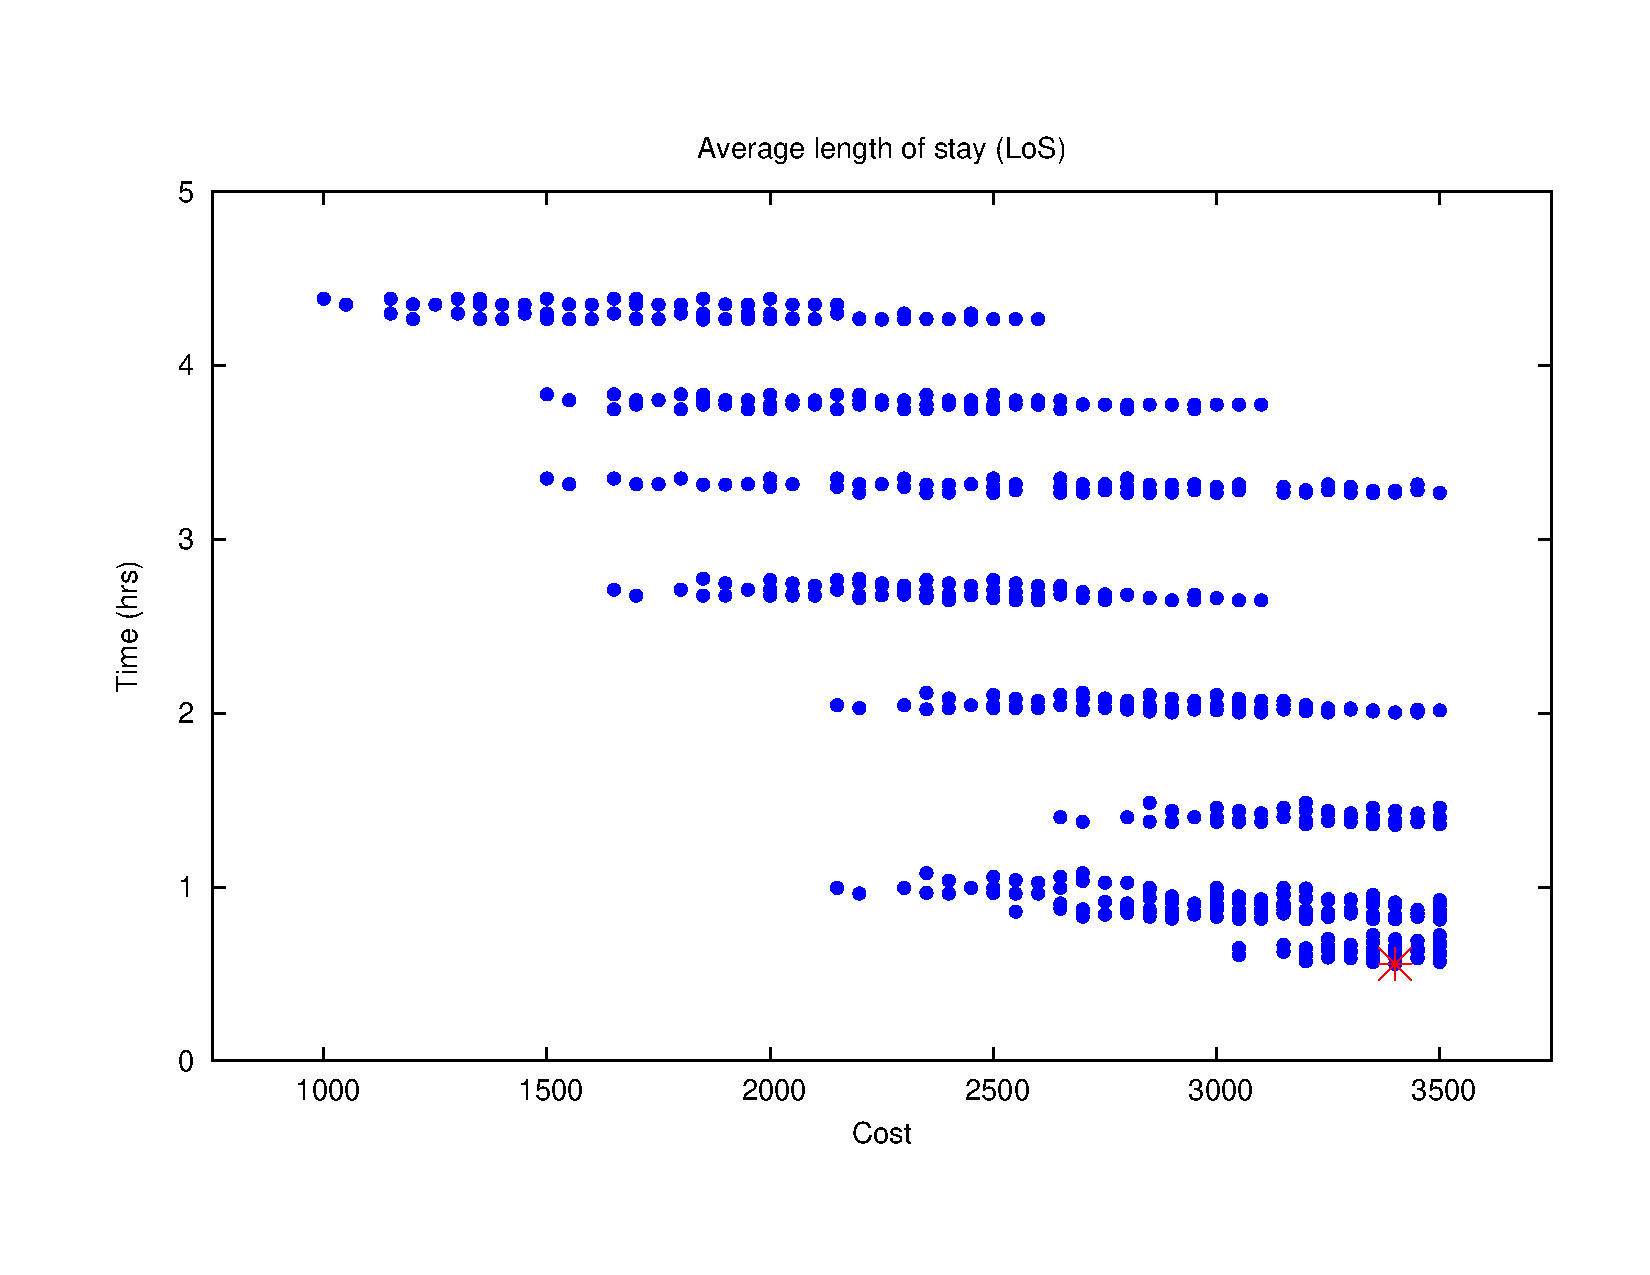
\includegraphics[width=0.95\columnwidth,height=0.25\paperheight]{figs4/v0/pipe-sorted-LoS_0-50_min}
\par\end{centering}

\caption{Average LoS obtained by the PA. The red triangle was the minimum.
\label{subfig:pipe8-1}}
\end{figure}
 The most important is the bottom region, in which the average minimum
LoS was around 1 hour. There were 180 configurations (from a total
of 602 in the feasible region) in this region, which is the one where
the minimum was.

The MC plus the K-means methods results are shown in \ref{subfig:mc8-1}
to \ref{subfig:km8-1}, respectively. The MC method found 125 configurations.
\begin{figure}[H]
\noindent \centering{}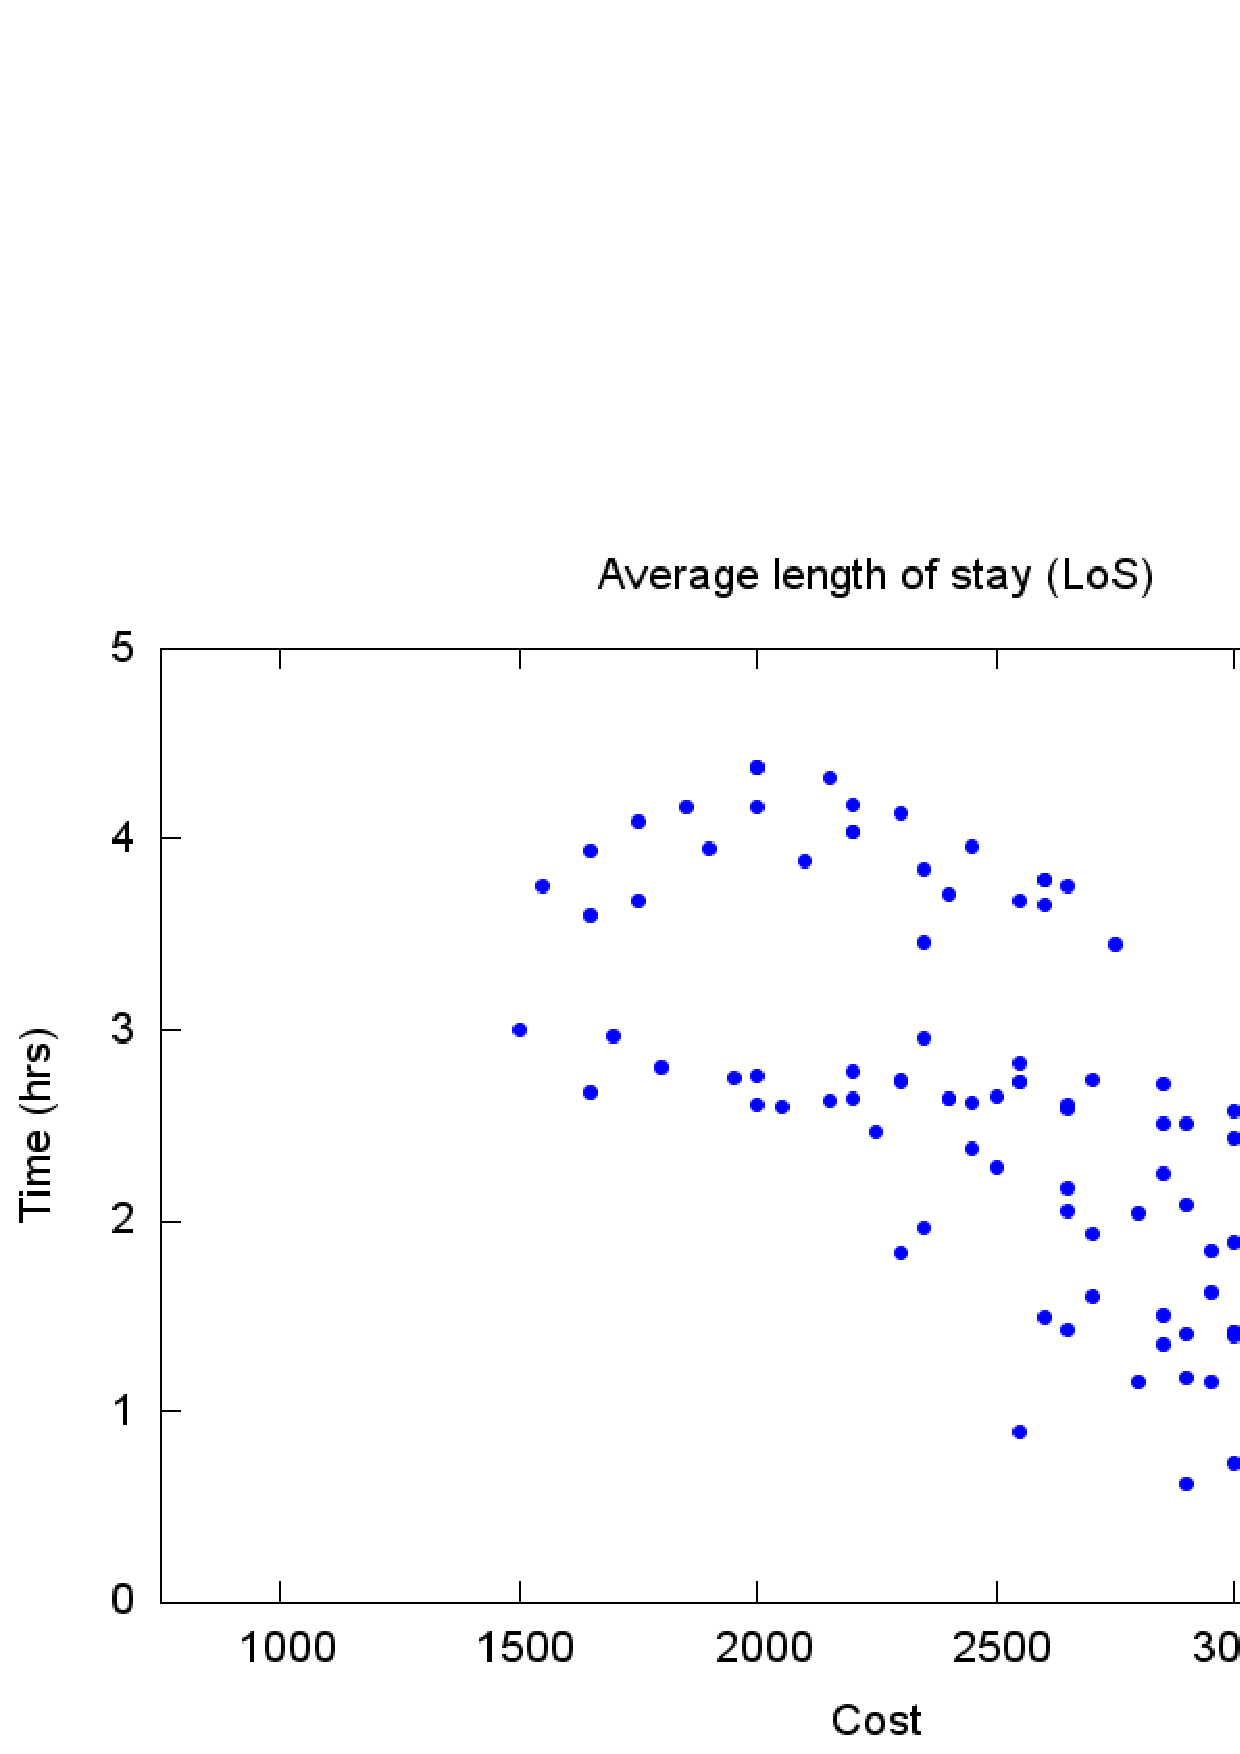
\includegraphics[width=0.95\columnwidth,height=0.25\paperheight]{figs4/v0/MC/MC-6400-602-50-69-25-125confs-LoS}\caption{Average LoS of 125 configurations obtained by the MC method. \label{subfig:mc8-1}}
\end{figure}
However, it was difficult to get any conclusion about such region;
therefore, the complementary K-means method was performed. The K-means
method identified two different clusters, shown in \ref{subfig:km8-1}.
The most important was the green cluster (at the bottom right), which
delimited the region where the optimum was.
\begin{figure}[H]
\noindent \centering{}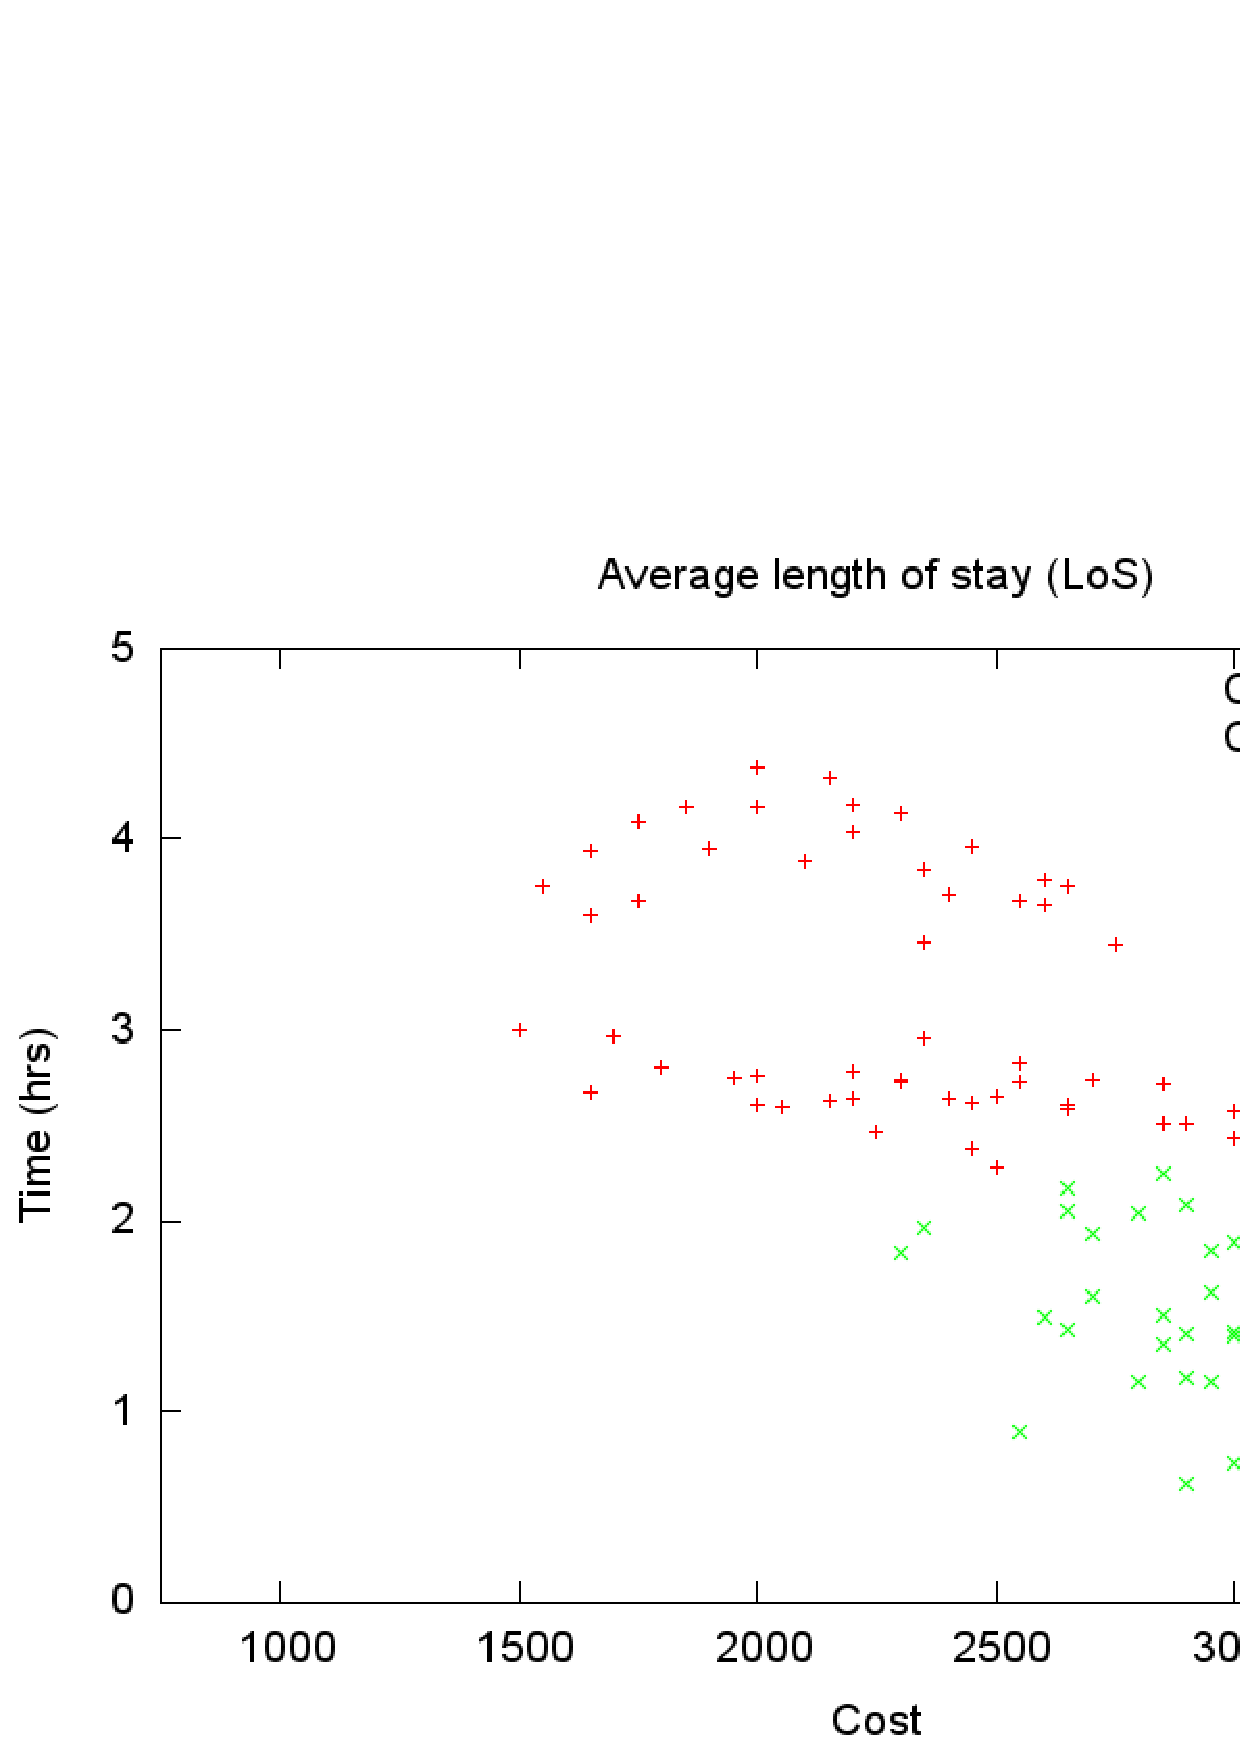
\includegraphics[width=0.95\columnwidth,height=0.25\paperheight]{figs4/v0/MC/K-means-6400-602-50-69-25-125-Cluster1-58_Cluster2-58}\caption{The K-means method identified two clusters of average LoS. The green
one delimited the region where the minimum was.\label{subfig:km8-1}}
\end{figure}


The \ref{fig:3D-scattered-graph-50} shows another way to visualise
the connectivity characteristic of the reduced regions found by the
proposed methodology. The axes of such graph are the equivalent operational
patient-service time ({\bf t$^*$}) of a ``single
one'' sanitary professional of each sanitary staff configuration
(the first column of \ref{subtab:As-pipe} to \ref{subtab:Ds-pipe},
where they were ordered by the PA \ref{eq:Pipeline formula}). In
such figure, the points of interest were the green points, which lie
in the region of interest, where the minimum was, which can be seen
in black triangle. It can be seen that it was not necessary to search
in the whole feasible region, but only in the green connected region.
\begin{figure}[H]
\noindent \begin{centering}
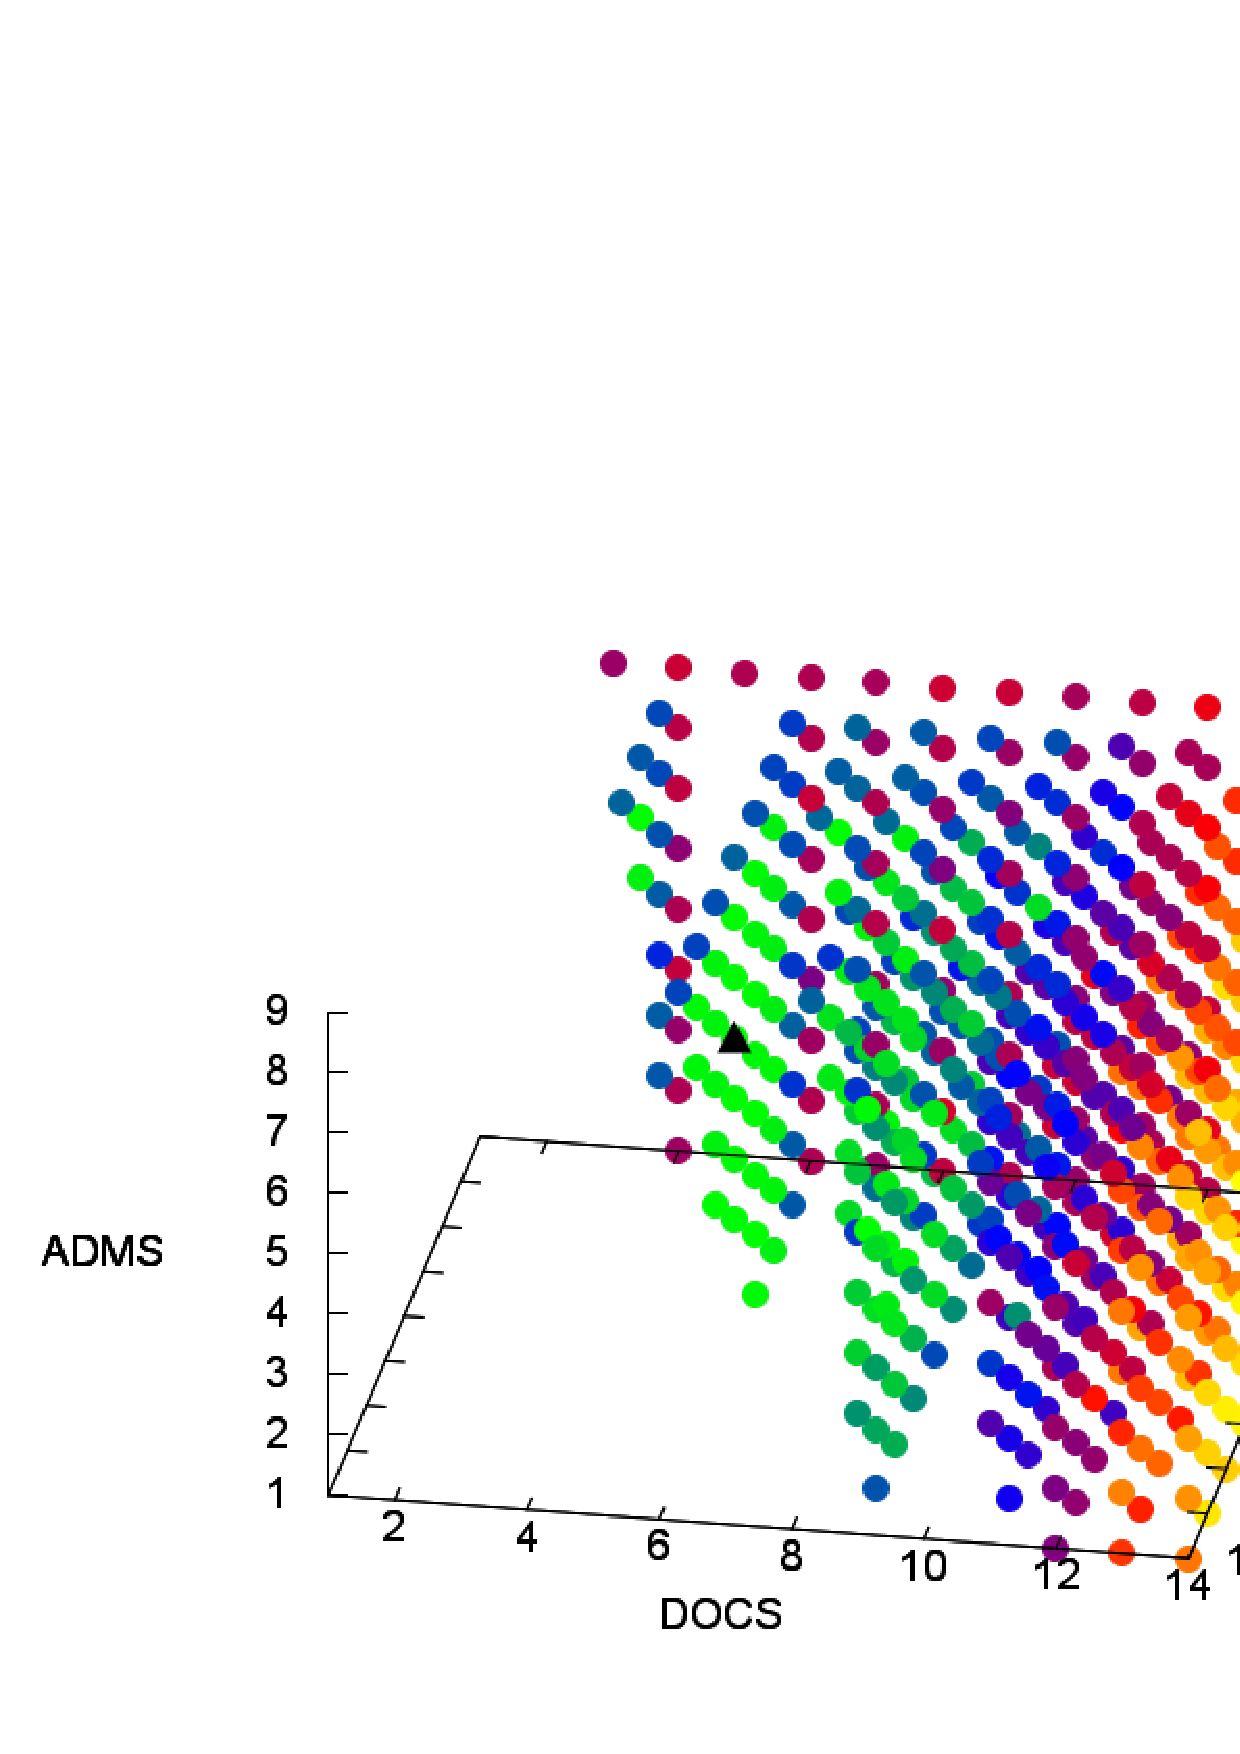
\includegraphics[width=0.95\columnwidth,height=0.2\paperheight]{figs4/v0/6400-602-50-3D-scatter-LoS2}
\par\end{centering}

\caption{3D scattered graph shows the average LoS index of the third workload
scenario (9 patients/hour). The average LoS index is expressed in
colour in hours.\label{fig:3D-scattered-graph-50}}
\end{figure}


Finally, after separately applied both the PA and the MC plus the
K-means methods, the \textquotedblleft{}reduced exhaustive search\textquotedblright{}
was separately performed in each reduced region identified. The optimum
found per each method: the ES, the PA, and the MC plus the K-means
methods are presented in \ref{tab:8p-a}, where the sanitary staff
configuration (doctors, nurses, and admission personnel), their associated
average minimum LoS, and cost configuration are shown. The three optima
 independently found were the same. 

\begin{comment}
Each staff configuration that got the minimum is presented in \ref{tab:4p-a},
\ref{tab:8p-a}, \ref{tab:12p-a}, and \ref{tab:16p-a}.
\end{comment}
\begin{comment}
\begin{figure}[h]
\hfill{}\subfloat[\label{subfloat:pipe8}Scattered 3D graph of doctors, nurses, and
admission personnel.]{

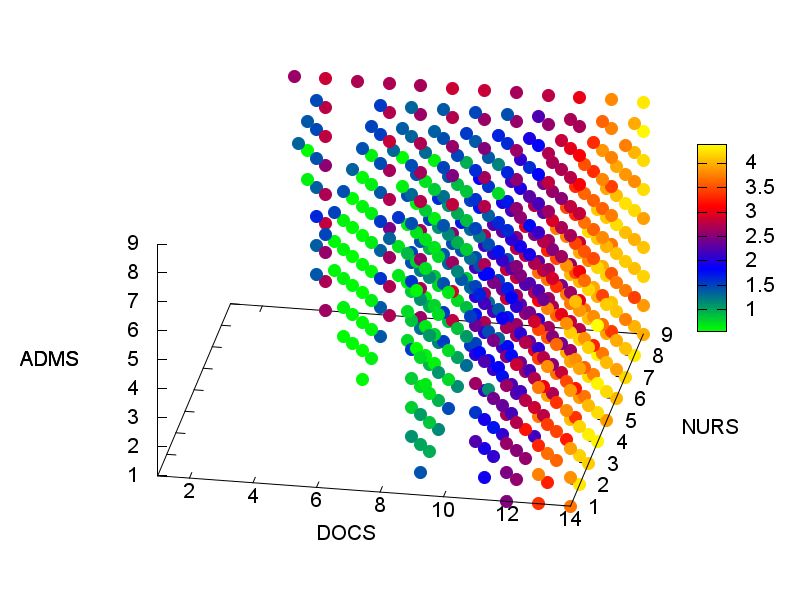
\includegraphics[width=0.48\columnwidth]{figs4/6400-602-50-3D-scatter-LoS.png}}\hfill{}\subfloat[\label{subfloat:contour8} Contour graph where doctors and nurses
can be seen.]{

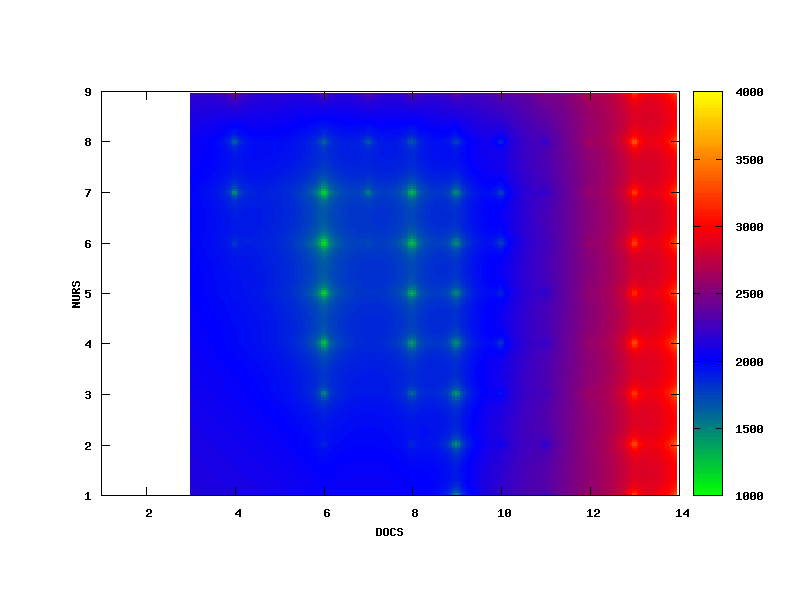
\includegraphics[width=0.48\columnwidth]{figs4/6400-602-50-sort-pipe_p5_y_p4-contour.png}}\hfill{}

\caption{\label{fig:Two-vision2} Graphs show the average LoS index of the
second workload scenario (9 patients/hour) using the first column
of \ref{subtab:As-pipe}, \ref{subtab:Ns-pipe}, and \ref{subtab:Ds-pipe},
where they were ordered by the pipeline approach (PA) \ref{eq:Pipeline formula}.
The colour bar is expresed in tics ( $hours\:=\frac{tics}{1000}$
). }
\end{figure}
\end{comment}
\vspace*{-.2cm}

\begin{table}[H]
\caption{Optimum staff configurations that got the average minimum LoS for
this workload scenario (up to 9 patients hourly), where S is Senior
and J is Junior. This optimum sanitary staff configuration is shown
in red triangle in \ref{subfig:es8-1} and in black triangle in \ref{fig:3D-scattered-graph-50}.}


\centering{}%
\begin{tabular}{cccccc>{\centering}p{2.8cm}}
\hline 
Method & euro & LoS (hrs) & D & N & A & Run time (hrs)

4 Pthreads\tabularnewline
\hline 
ES & 3,350  & 0.55 & 4J & 2S & 1S,1J & 1.57\tabularnewline
PA & 3,350  & 0.55 & 4J & 2S & 1S,1J & 0.39\tabularnewline
MC+K-means & 3,350  & 0.55 & 4J & 2S & 1S,1J & 1.01\tabularnewline
\hline 
\end{tabular}\label{tab:8p-a} 
\end{table}


\clearpage{}


\subsubsection{Third Workload Scenario}

The results of this scenario, up to 13 patients/hour, are shown from
\ref{subfig:es13-1} to \ref{subfig:km13-1}. The ES result is shown
in \ref{subfig:es13-1}, where the red triangle was the minimum.
\begin{figure}[H]
\noindent \begin{centering}
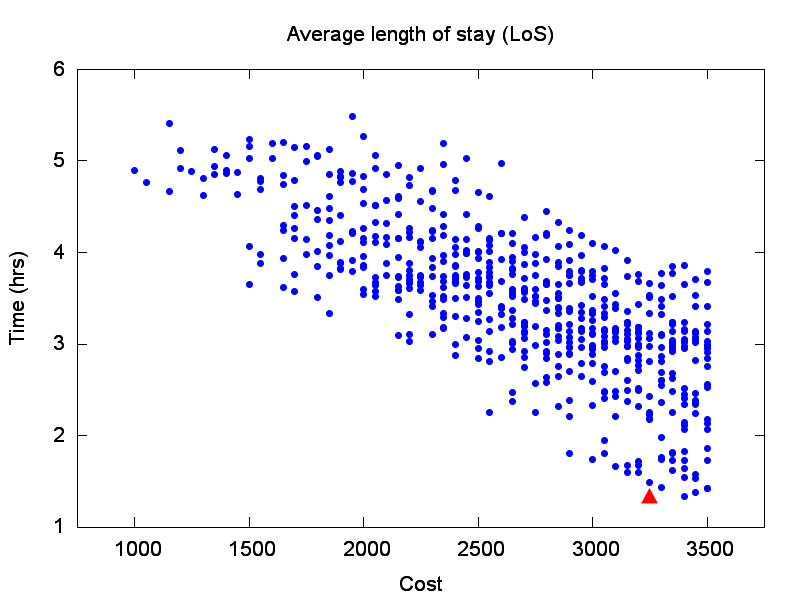
\includegraphics[width=0.95\columnwidth,height=0.25\paperheight]{figs4/v0/6400-602-75-exh-LoS-min}
\par\end{centering}

\caption{Average LoS obtained by the ES. The red triangle was the minimum.
\label{subfig:es13-1}}
\end{figure}


The PA result is shown in \ref{subfig:pipe13-1}, where many regions
can be clearly seen and the red triangle is the minimum. 
\begin{figure}[H]
\noindent \begin{centering}
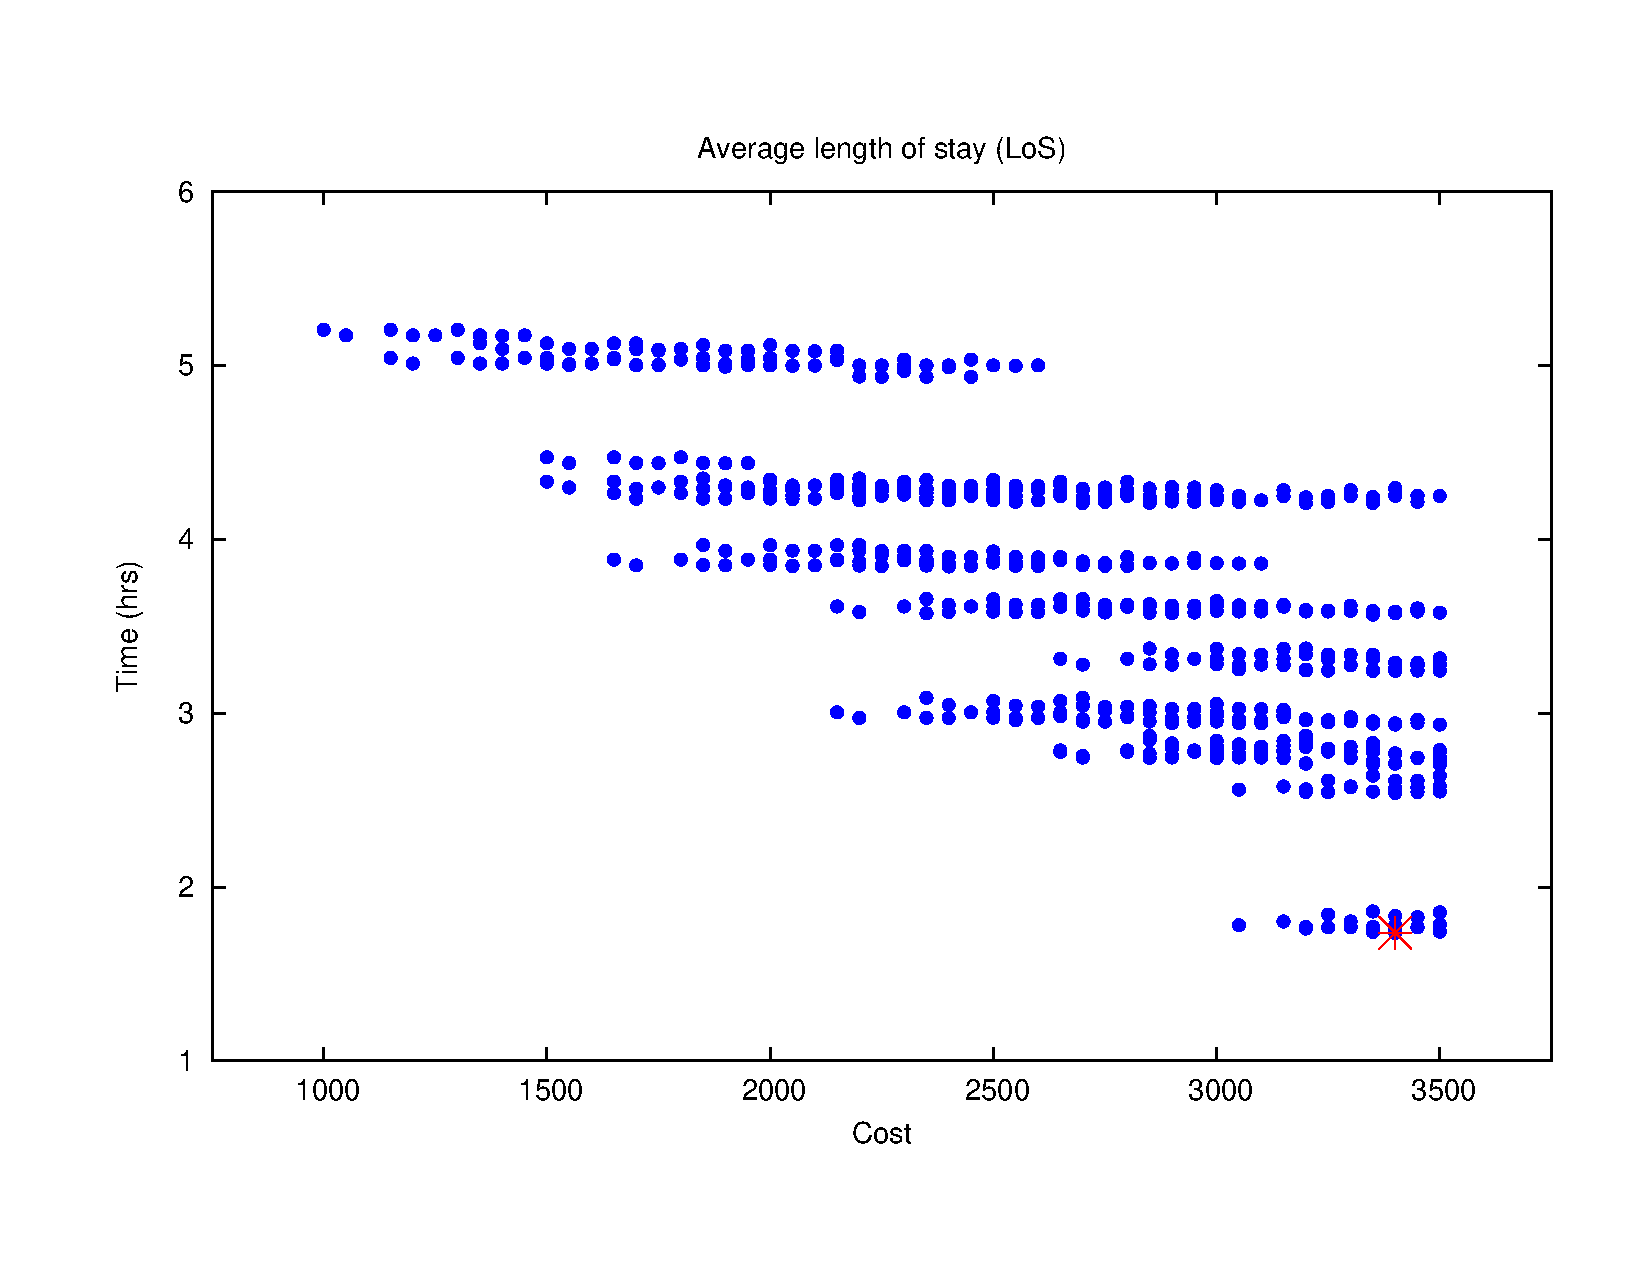
\includegraphics[width=0.95\columnwidth,height=0.25\paperheight]{figs4/v0/pipe-sorted-LoS_0-75_min}
\par\end{centering}

\caption{Average LoS obtained by the PA. The red triangle was the minimum.
\label{subfig:pipe13-1}}
\end{figure}
 The most important is the bottom region, in which the average minimum
LoS was less than 2 hours. There were 21 configurations (from a total
of 602 in the feasible region) in this region, which is the one where
the minimum was.

The MC plus the K-means methods results are shown in \ref{subfig:mc13-1}
to \ref{subfig:km13-1}, respectively. The MC method found 125 configurations.
\begin{figure}[H]
\noindent \centering{}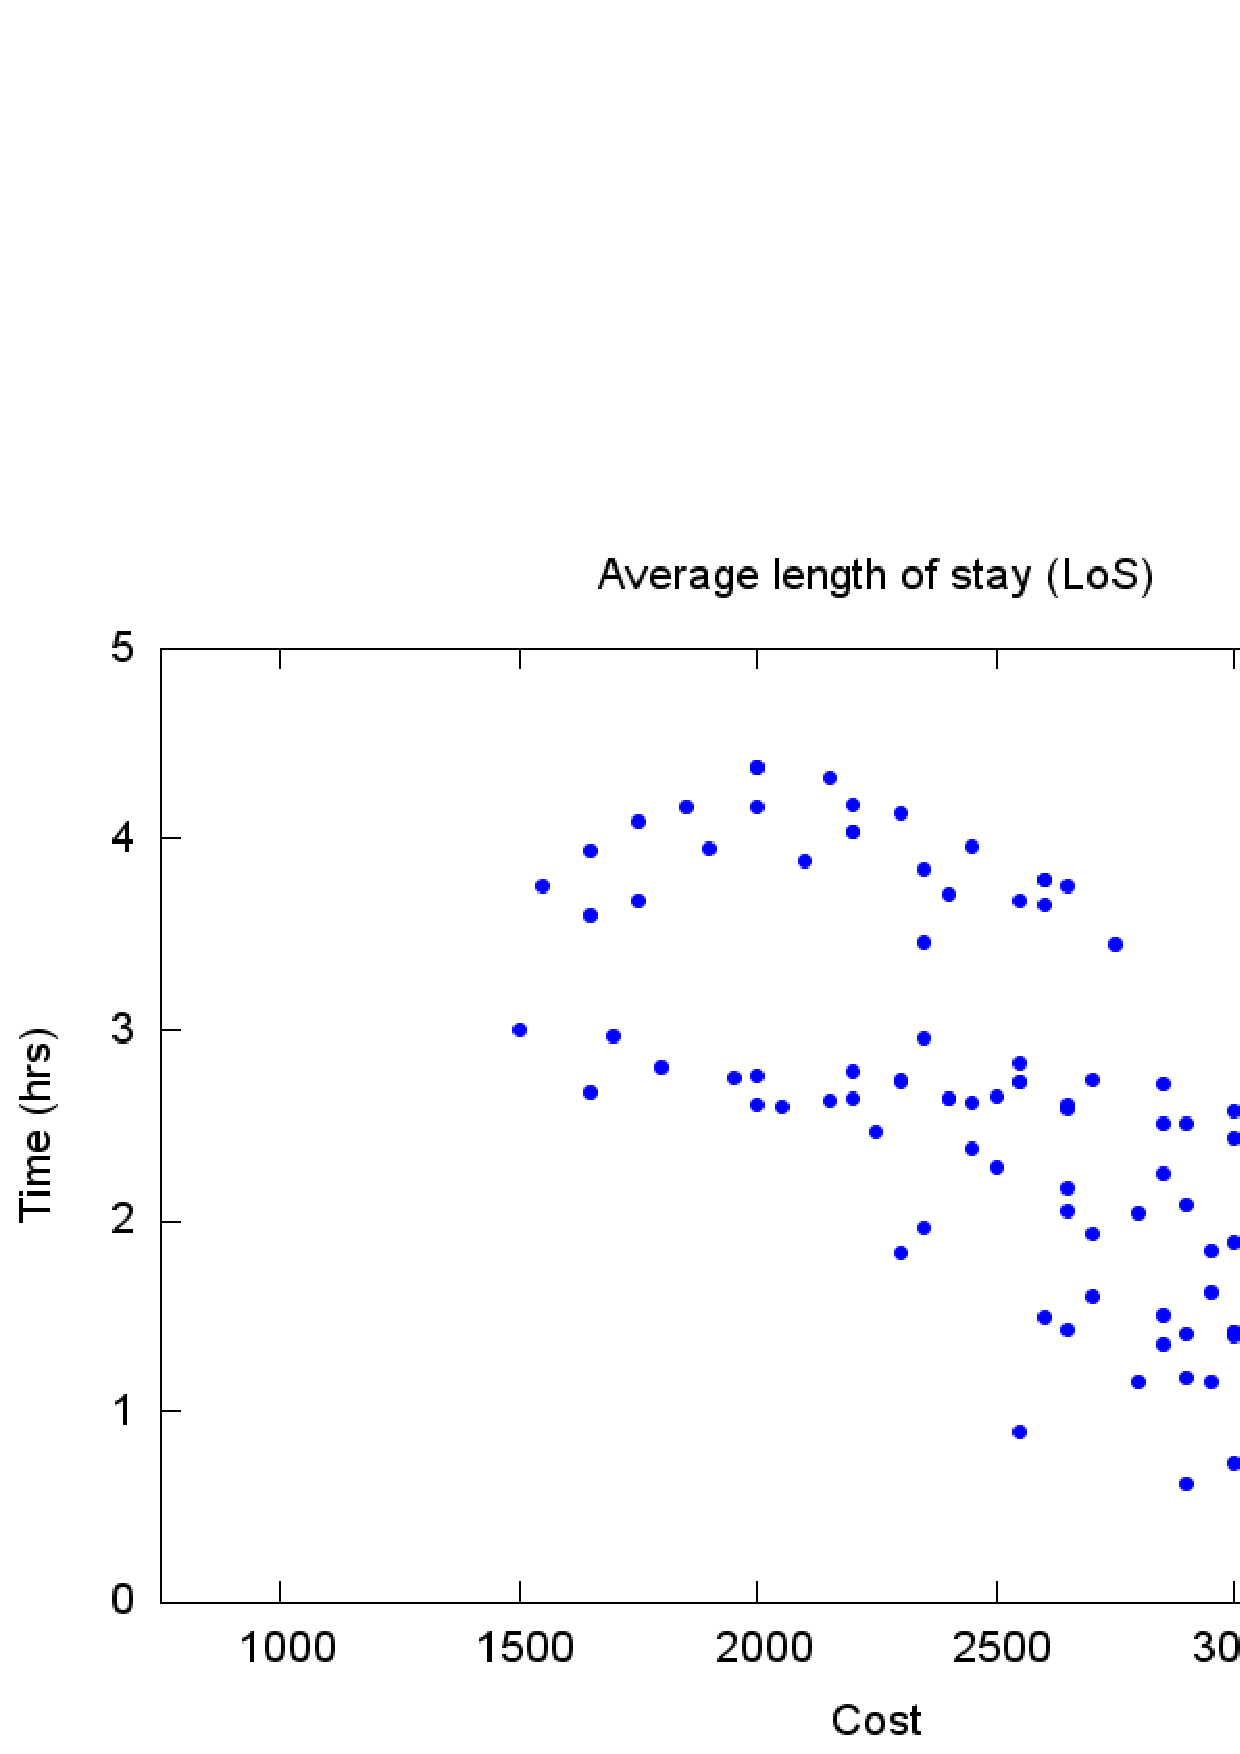
\includegraphics[width=0.95\columnwidth,height=0.25\paperheight]{figs4/v0/MC/MC-6400-602-50-69-25-125confs-LoS}\caption{Average LoS of 125 configurations obtained by the MC method. \label{subfig:mc13-1}}
\end{figure}
 However, it was difficult to get any conclusion about such region;
therefore, the complementary K-means method was performed. The K-means
method identified two different clusters, shown in \ref{subfig:km13-1}.
The most important was the green cluster (at the bottom right), which
delimited the region where the optimum was.
\begin{figure}[H]
\noindent \centering{}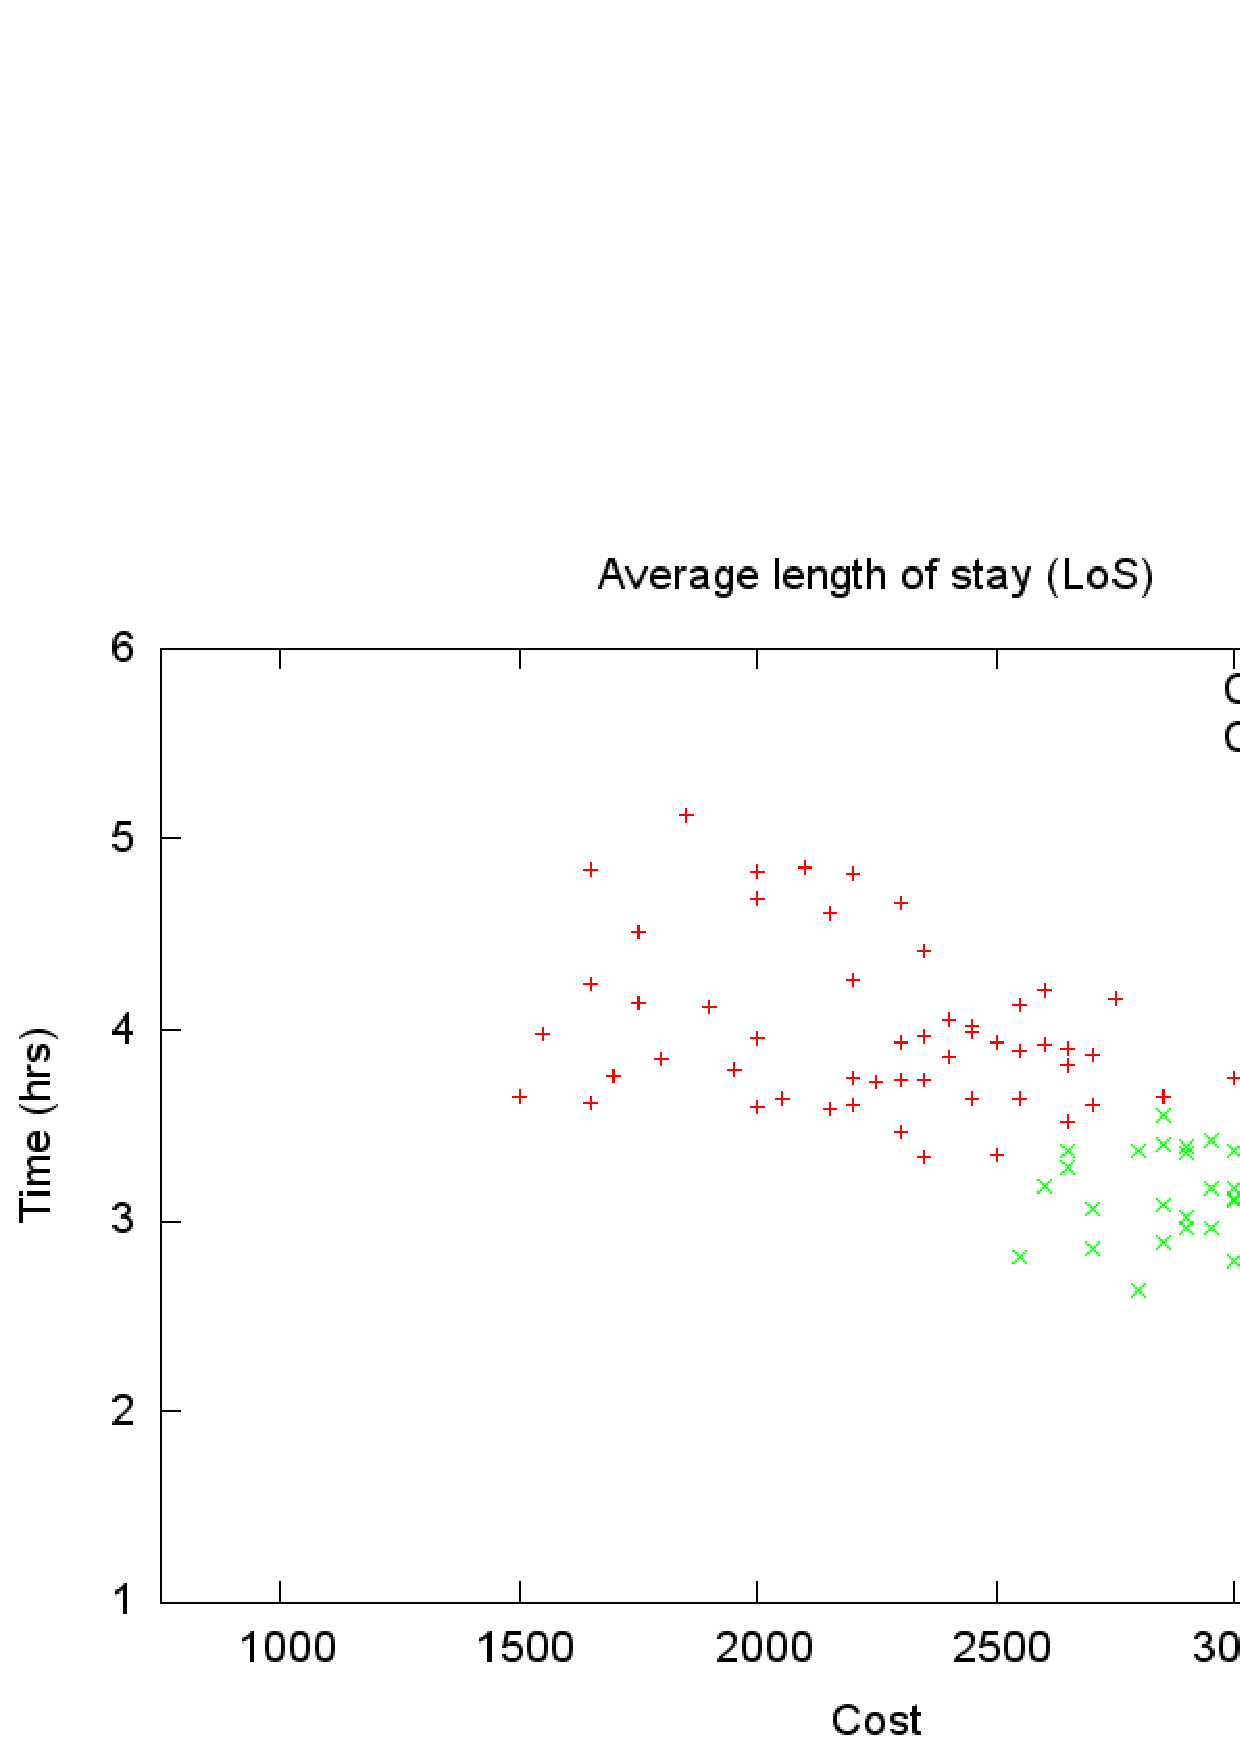
\includegraphics[width=0.95\columnwidth,height=0.25\paperheight]{figs4/v0/MC/K-means-6400-602-75-69-25-125-Cluster1-54_Cluster2-63}\caption{The K-means method identified two clusters of average LoS. The green
one delimited the region where the minimum was.\label{subfig:km13-1}}
\end{figure}


The \ref{fig:3D-scattered-graph-75} shows another way to visualise
the connectivity characteristic of the reduced regions found by the
the proposed methodology. The axes of such graph are the equivalent
operational patient-service time ({\bf t$^*$})
of a ``single one'' sanitary professional of each sanitary staff
configuration (the first column of \ref{subtab:As-pipe} to \ref{subtab:Ds-pipe},
where they were ordered by the PA \ref{eq:Pipeline formula}). In
such figure, the points of interest were the green points, which lie
in the region of interest, where the minimum was, which can be seen
in black triangle. It can be seen that it was not necessary to search
in the whole feasible region, but only in the green connected region.
\begin{figure}[h]
\noindent \centering{}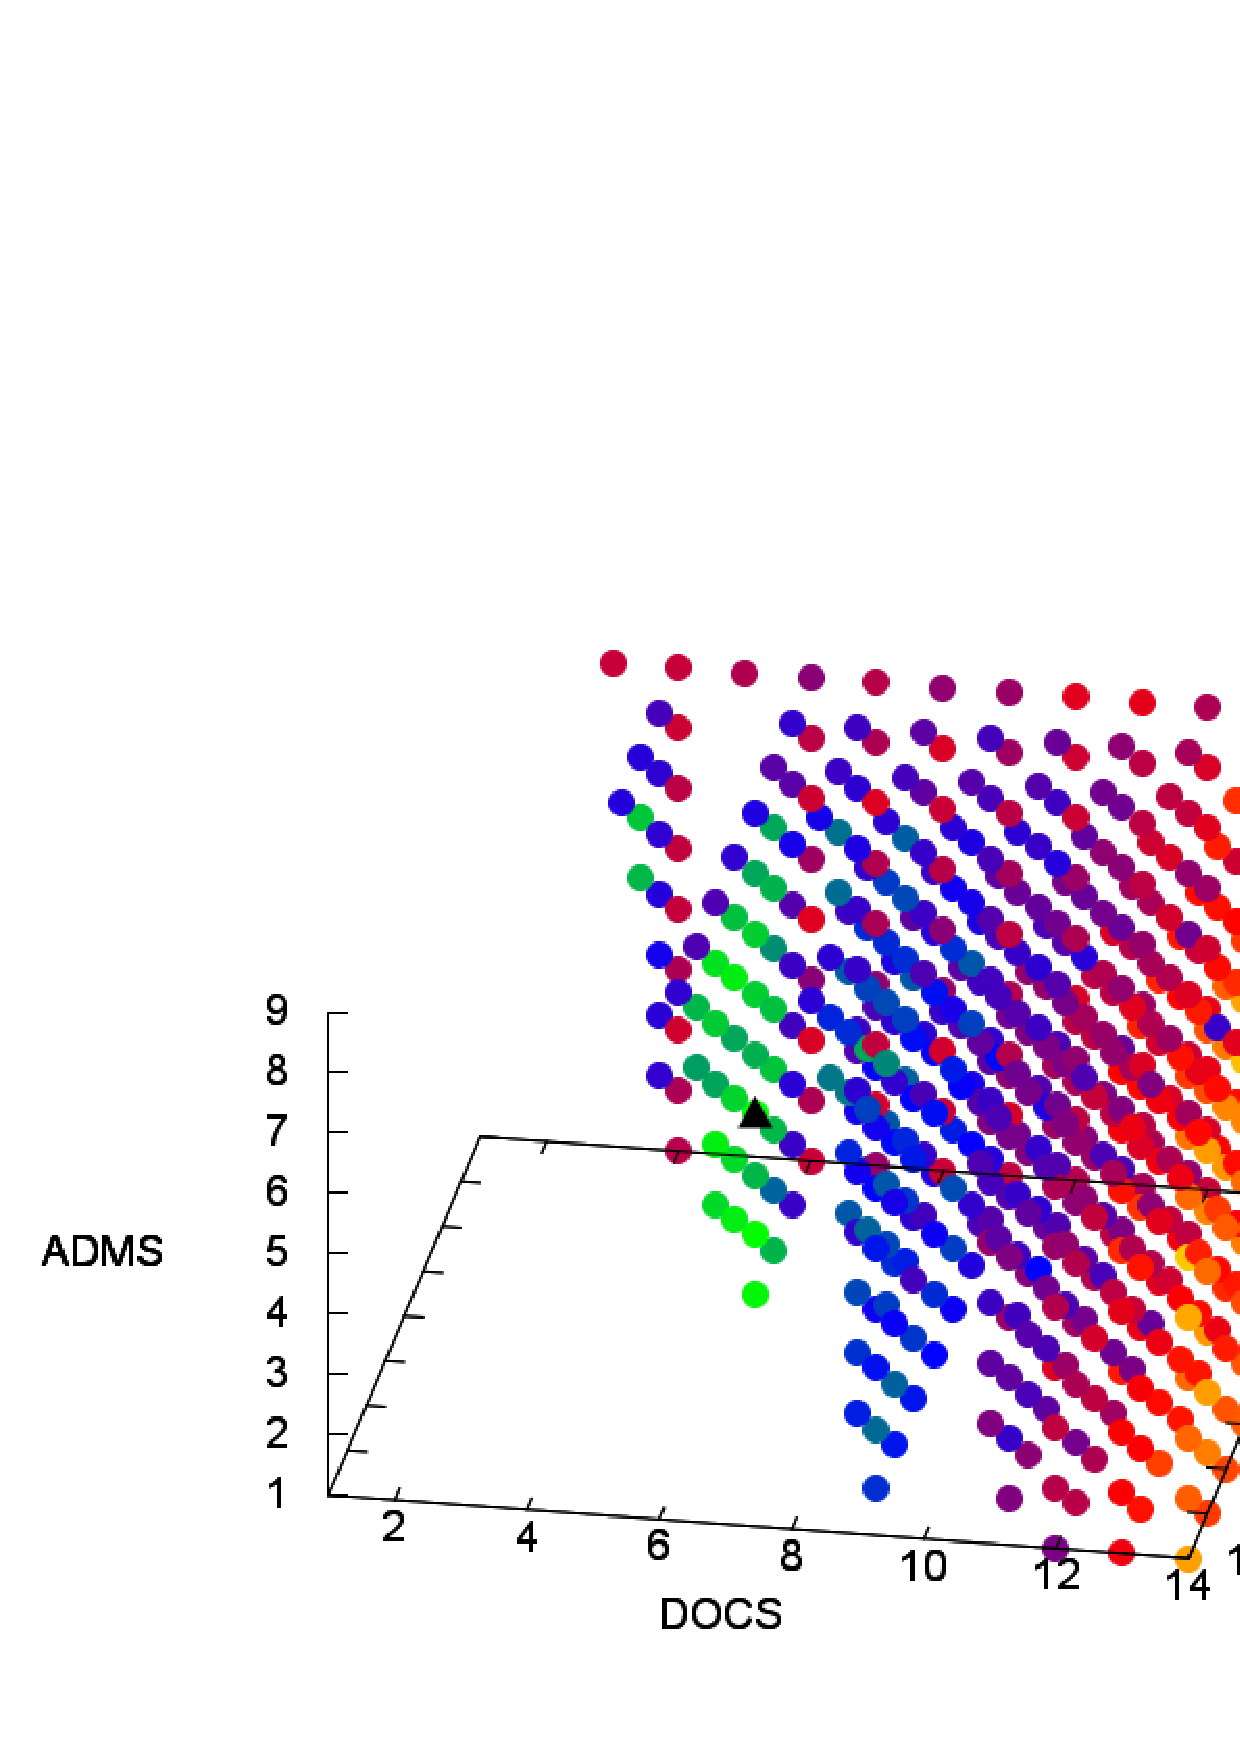
\includegraphics[width=0.88\columnwidth,height=0.2\paperheight]{figs4/v0/6400-602-75-3D-scatter-LoS2}\caption{3D scattered graph shows the average LoS index of the third workload
scenario (13 patients/hour). The average LoS index is expressed in
colour in hours. \label{fig:3D-scattered-graph-75}}
\end{figure}


Finally, after separately applied both the PA and the MC plus the
K-means methods, the \textquotedblleft{}reduced exhaustive search\textquotedblright{}
was separately performed in each reduced region identified. The optimum
found per each method: the ES, the PA, and the MC plus the K-means
methods are presented in \ref{tab:12p-a}, where the sanitary staff
configuration (doctors, nurses, and admission personnel), their associated
average minimum LoS, and cost configuration are shown. The three optima
independently found were the same. 

\begin{comment}
Each staff configuration that got the minimum is presented in \ref{tab:4p-a},
\ref{tab:8p-a}, \ref{tab:12p-a}, and \ref{tab:16p-a}.
\end{comment}
\vspace*{-.2cm}%
\begin{comment}
\begin{figure}[h]
\noindent \begin{centering}
\begin{minipage}[t][1\totalheight][s]{0.48\linewidth}%
\noindent \begin{center}
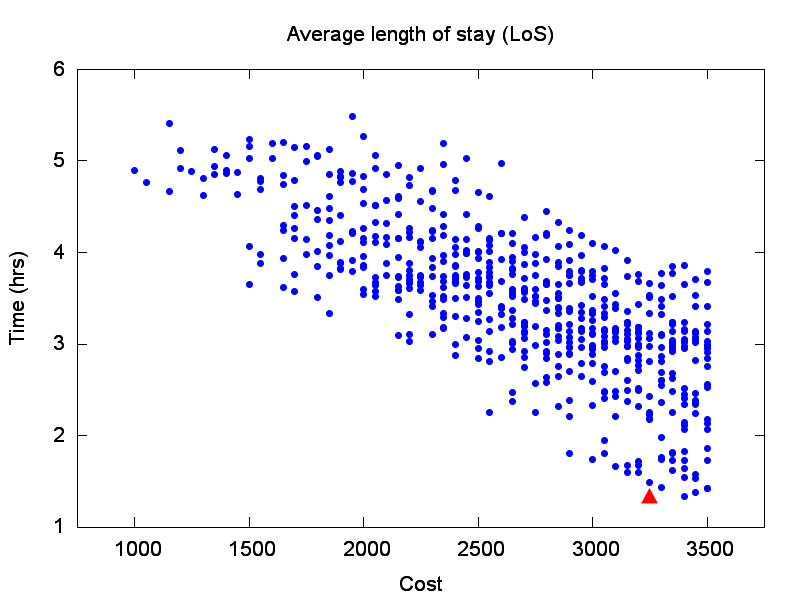
\includegraphics[width=1\columnwidth]{figs4/v0/6400-602-75-exh-LoS-min.png}
\par\end{center}

\vspace*{-1cm}

\noindent \begin{center}
\caption{Average LoS obtained by the ES method. The red triangle was the minimum.
\label{subfig:es12}}

\par\end{center}%
\end{minipage}\hfill{}%
\begin{minipage}[t][1\totalheight][s]{0.48\linewidth}%
\noindent \begin{center}
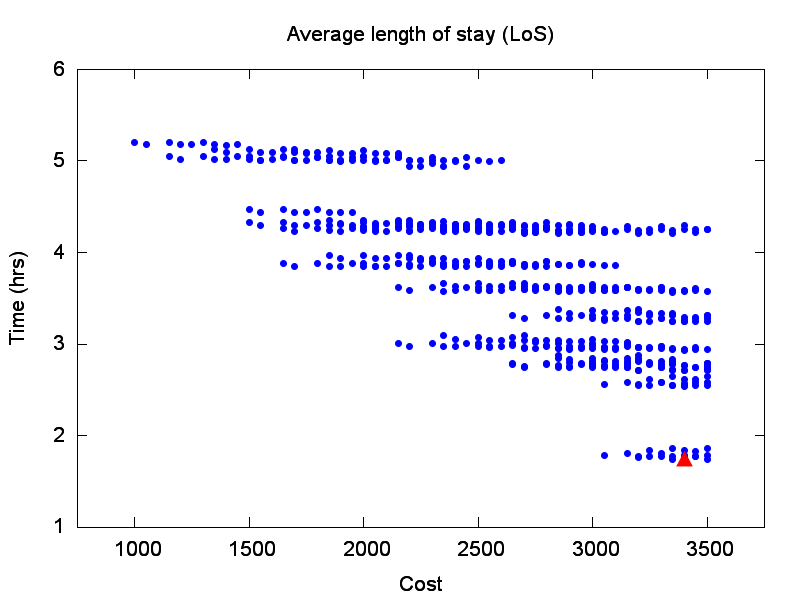
\includegraphics[width=1\columnwidth]{figs4/v0/pipe-sorted-LoS_0.75_min.png}
\par\end{center}

\vspace*{-1cm}

\noindent \begin{center}
\caption{Average LoS obtained by the PA. The red triangle was the minimum.\label{subfig:pipe12}}

\par\end{center}%
\end{minipage}
\par\end{centering}

\noindent \begin{centering}
%\centering\vspace{0cm}
\vspace*{-1.2cm}
\par\end{centering}

\begin{minipage}[t][1\totalheight][s]{0.48\textwidth}%
\noindent \begin{center}
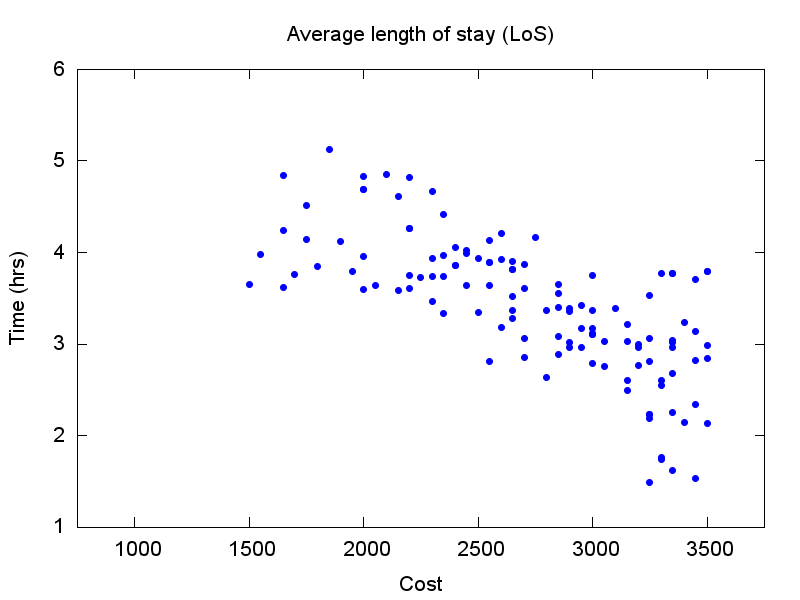
\includegraphics[width=1\columnwidth]{figs4/v0/MC/MC-6400-602-75-69-25-125confs-LoS.png}
\par\end{center}

\vspace*{-0.8cm}

\caption{Average LoS of 125 configurations obtained by the MC method.\label{subfig:mc12-1}}
%
\end{minipage}\hfill{}%
\begin{minipage}[t][1\totalheight][s]{0.48\textwidth}%
\noindent \begin{center}
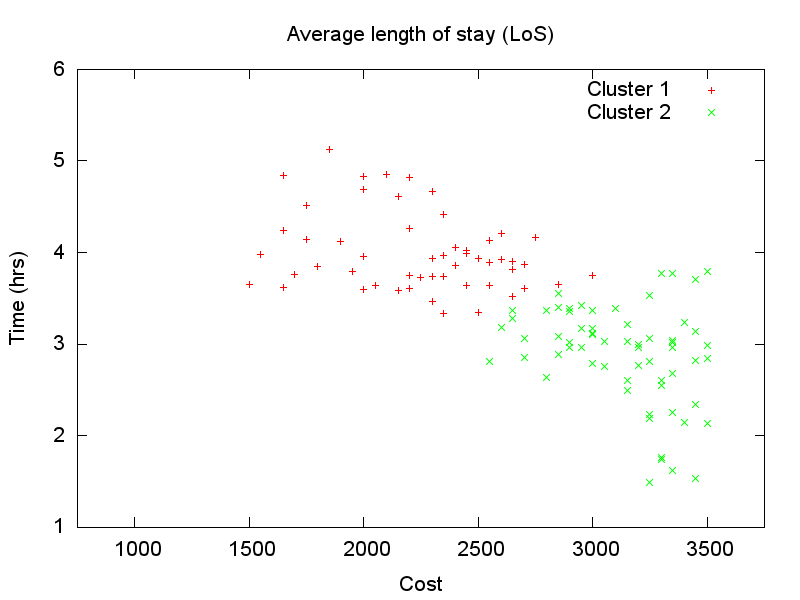
\includegraphics[width=1\columnwidth]{figs4/v0/MC/K-means-6400-602-75-69-25-125-Cluster1-54_Cluster2-63.png}
\par\end{center}

\vspace*{-0.8cm}

\caption{The K-means method identified two clusters of average LoS. The green
one delimited the region where the minimum was.\label{subfig:km12-1}}
%
\end{minipage}

\vspace*{0.4cm}{\bf Figures} show the average LoS of the third workload scenario (13 patients/hour) using the ES, the PA, and the MC+K-means methods.
\end{figure}
\end{comment}
\begin{comment}
\begin{figure}[h]
\hfill{}\subfloat[\label{subfloat:pipe12} Scattered 3D graph of doctors, nurses, and
admission personnel.]{

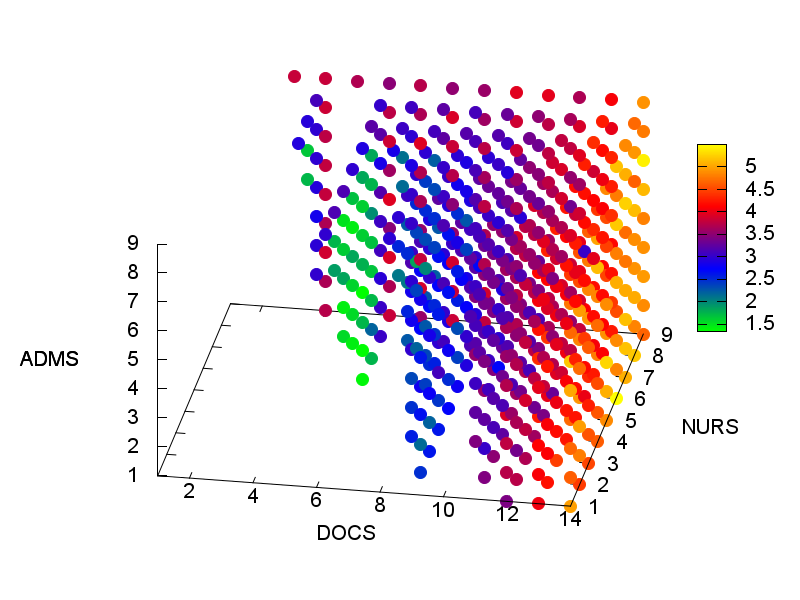
\includegraphics[width=0.48\columnwidth]{figs4/6400-602-75-3D-scatter-LoS.png}}\hfill{}\subfloat[\label{subfloat:contour12} Contour graph where doctors and nurses
can be seen.]{

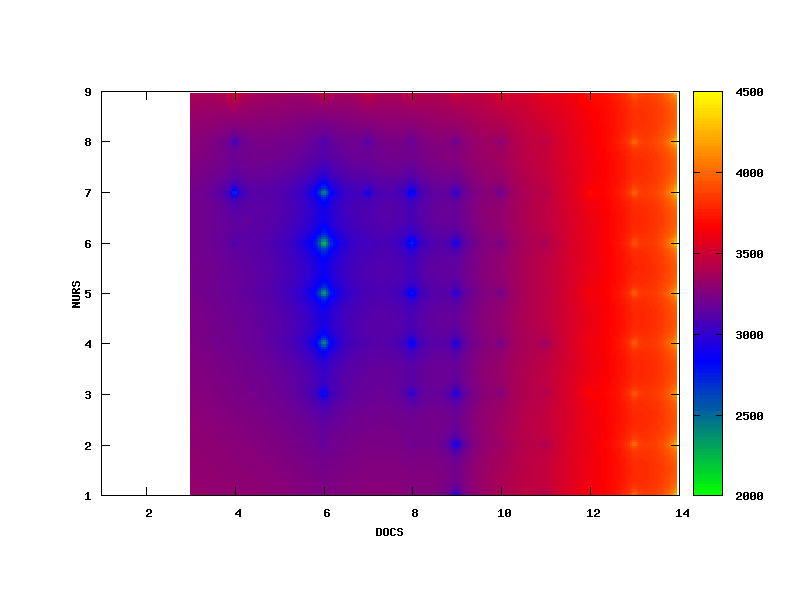
\includegraphics[width=0.48\columnwidth]{figs4/6400-602-75-sort-pipe_p5_y_p4-contour.png}}\hfill{}

\caption{\label{fig:Two-vision3} Graphs show the average LoS index of the
third workload scenario (13 patients/hour) using the first column
of \ref{subtab:As-pipe}, \ref{subtab:Ns-pipe}, and \ref{subtab:Ds-pipe},
where they were ordered by the pipeline approach (PA) \ref{eq:Pipeline formula}.
The colour bar is expresed in tics ( $hours\:=\frac{tics}{1000}$
). }
\end{figure}
\end{comment}


\begin{table}[h]
\caption{Optimum staff configurations that got the average minimum LoS for
this workload scenario (up to 13 patients hourly), where S is Senior
and J is Junior. This optimum sanitary staff configuration is shown
in red triangle in \ref{subfig:es13-1} and in black triangle in \ref{fig:3D-scattered-graph-75}.}


\begin{centering}
\begin{tabular}{cccccc>{\centering}p{2.8cm}}
\hline 
Method & euro & LoS (hrs) & D & N & A & Run time (hrs)

4 Pthreads\tabularnewline
\hline 
ES & 3,250 & 1.33 & 4J & 1S,1J & 2S & 2.45\tabularnewline
PA & 3,250 & 1.33 & 4J & 1S,1J & 2S & 0.16\tabularnewline
MC+K-means & 3,250 & 1.33 & 4J & 1S,1J & 2S & 1.49\tabularnewline
\hline 
\end{tabular}
\par\end{centering}

\label{tab:12p-a} 
\end{table}


\clearpage{}


\subsubsection{Fourth Workload Scenario}

The results of this scenario, up to 17 patients/hour, are shown from
\ref{subfig:es17-1} to \ref{subfig:km17-1}. The ES result is shown
in \ref{subfig:es17-1}, where the red triangle is the minimum. 
\begin{figure}[H]
\noindent \begin{centering}
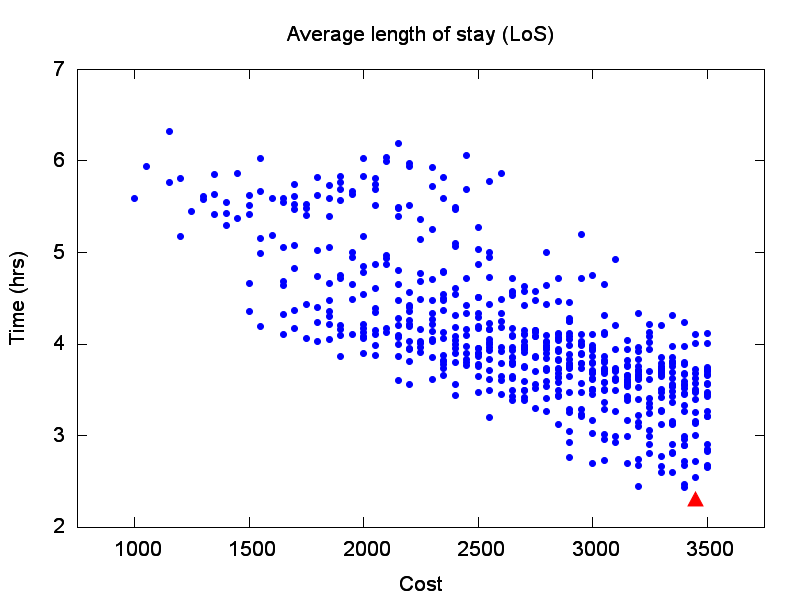
\includegraphics[width=0.95\columnwidth,height=0.25\paperheight]{figs4/v0/6400-602-100-exh-LoS-min}
\par\end{centering}

\caption{Average LoS obtained by the ES. The red triangle was the minimum.
\label{subfig:es17-1}}
\end{figure}


The PA result is shown in \ref{subfig:pipe17-1}, where many regions
can be clearly seen and the red triangle is the minimum.
\begin{figure}[H]
\noindent \begin{centering}
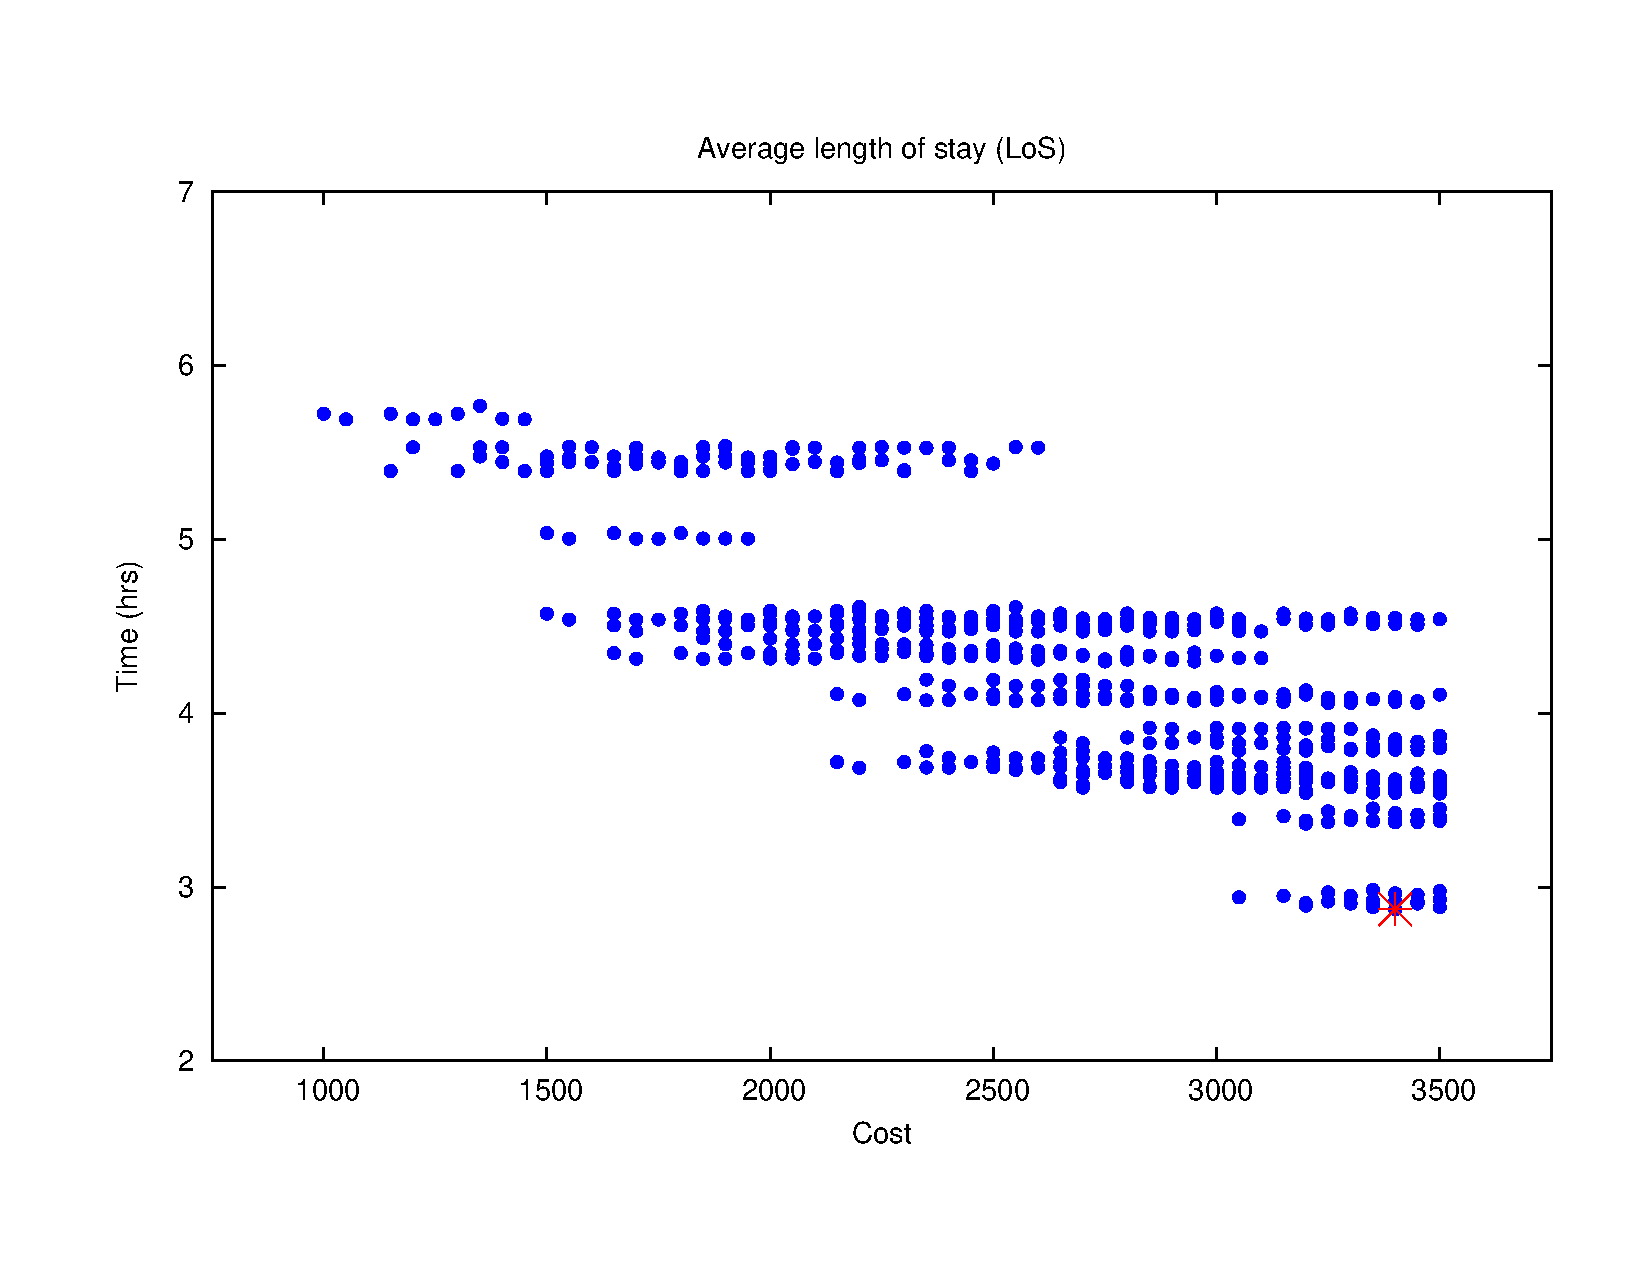
\includegraphics[width=0.95\columnwidth,height=0.25\paperheight]{figs4/v0/pipe-sorted-LoS_1_0_min}
\par\end{centering}

\caption{Average LoS obtained by the PA. The red triangle was the minimum.
\label{subfig:pipe17-1}}
\end{figure}
 The most important is the bottom region, in which the average minimum
LoS was around than 3 hours. There were 21 configurations (from a
total of 602 in the feasible region) in this region, which is the
one where the maximum was.

The MC plus the K-means methods results are shown in \ref{subfig:mc17-1}
to \ref{subfig:km17-1}, respectively. The MC method found 125 configurations.
\begin{figure}[H]
\noindent \centering{}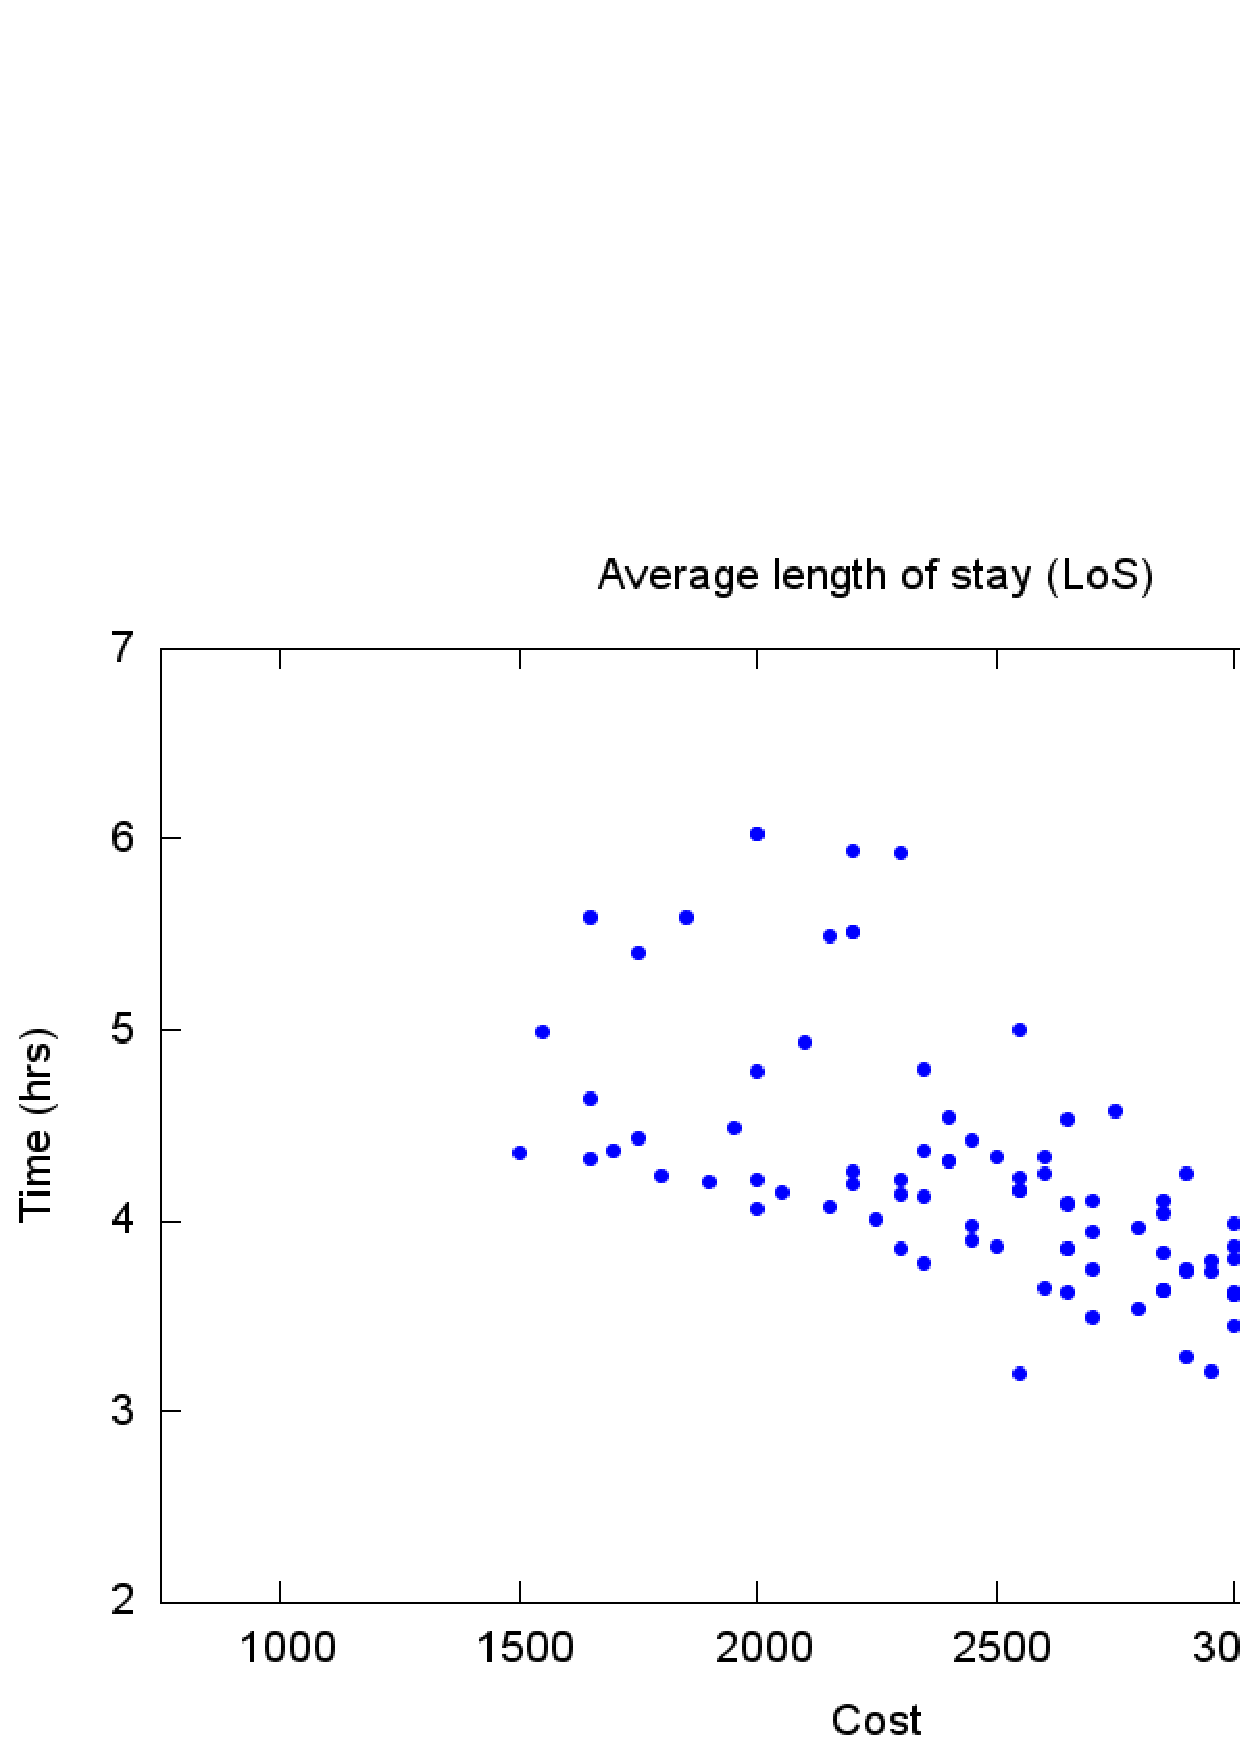
\includegraphics[width=0.95\columnwidth,height=0.25\paperheight]{figs4/v0/MC/MC-6400-602-100-69-25-125confs-LoS}\caption{Average LoS of 125 configurations obtained by the MC method. \label{subfig:mc17-1}}
\end{figure}
 However, it was difficult to get any conclusion about such region;
therefore, the complementary K-means method was performed. The K-means
method identified two different clusters, shown in \ref{subfig:km17-1}.
The most important was the green cluster (at the bottom right), which
delimited the region where the optimum was.
\begin{figure}[H]
\noindent \centering{}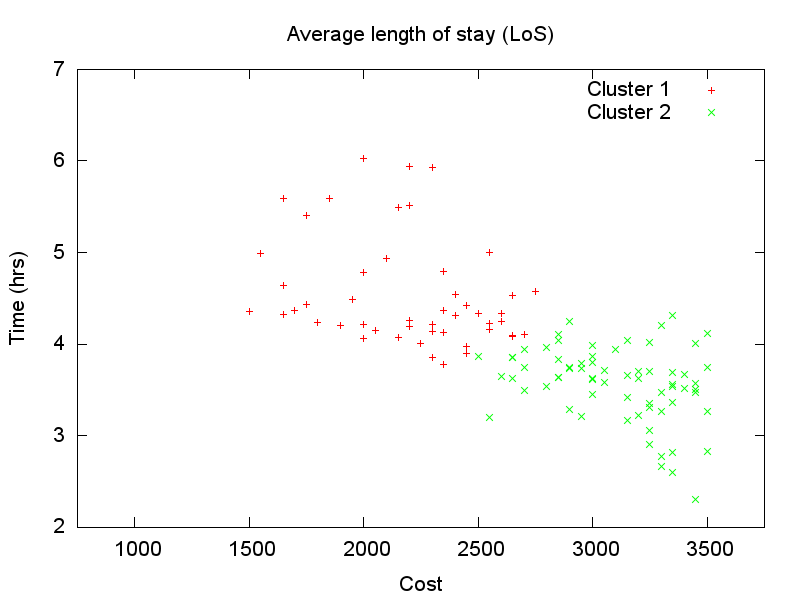
\includegraphics[width=0.95\columnwidth,height=0.25\paperheight]{figs4/v0/MC/K-means-6400-602-100-69-25-125-Cluster1-49_Cluster2-68}\caption{The K-means method identified two clusters of average LoS. The green
one delimited the region where the minimum was.\label{subfig:km17-1}}
\end{figure}


The \ref{fig:3D-scattered-graph-100} shows another way to visualise
the connectivity characteristic of the reduced regions found by the
proposed methodology. The axes of such graph are the equivalent operational
patient-service time ({\bf t$^*$}) of a ``single
one'' sanitary professional of each sanitary staff configuration
(the first column of \ref{subtab:As-pipe} to \ref{subtab:Ds-pipe},
where they were ordered by the PA \ref{eq:Pipeline formula}). In
such figure, the points of interest were the green points, which lie
in the region of interest, where the minimum was, which can be seen
in black triangle. It can be seen that it was not necessary to search
in the whole feasible region, but only in the green connected region.
\begin{figure}[h]
\noindent \centering{}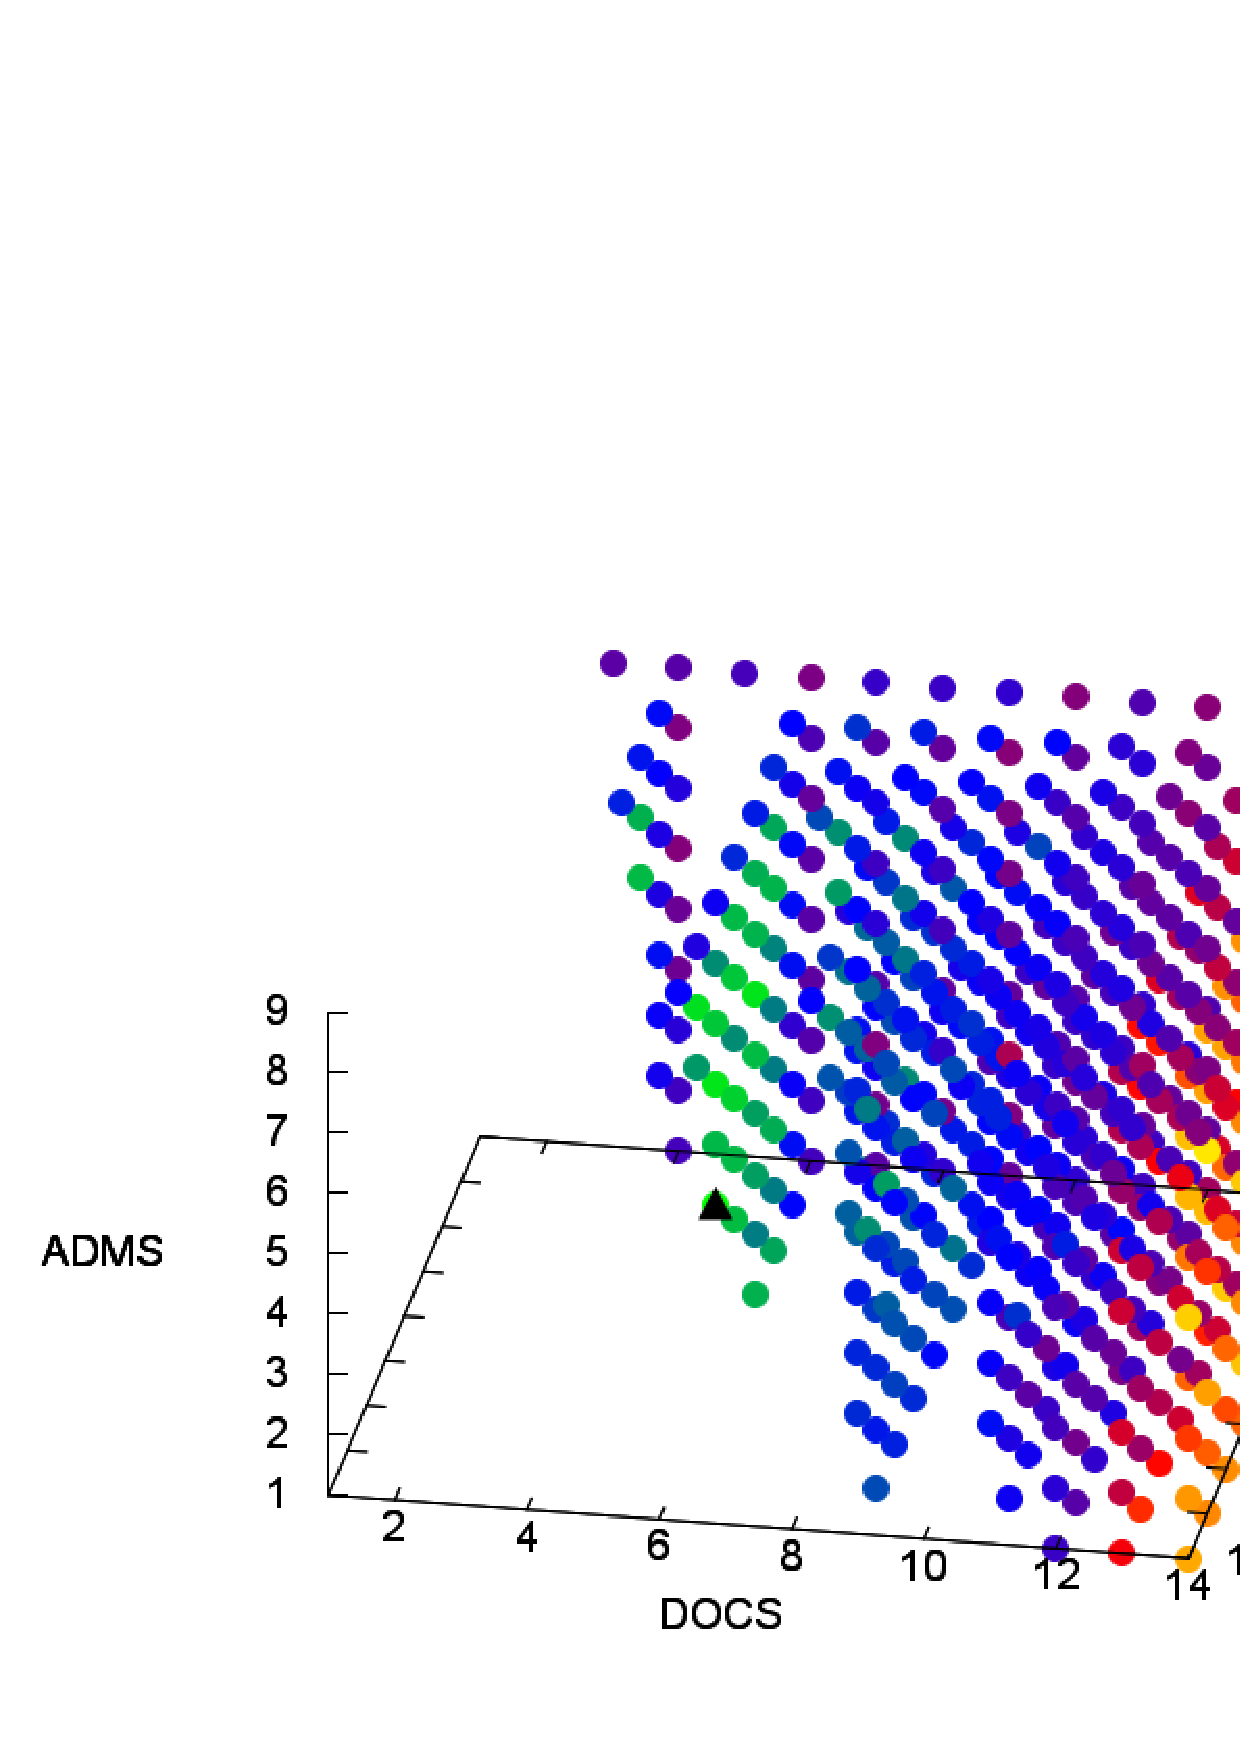
\includegraphics[width=0.88\columnwidth,height=0.2\paperheight]{figs4/v0/6400-602-100-3D-scatter-LoS2}\caption{3D scattered graph shows the average LoS index of the third workload
scenario (17 patients/hour). The average LoS index is expressed in
colour in hours. \label{fig:3D-scattered-graph-100}}
\end{figure}


Finally, after separately applied both the PA and the MC plus the
K-means methods, the \textquotedblleft{}reduced exhaustive search\textquotedblright{}
was separately performed in each reduced region identified.The optimum
found per each method: the ES, the PA, and the MC plus the K-means
methods are presented in \ref{tab:16p-a}, where the sanitary staff
configuration (doctors, nurses, and admission personnel), their associated
average minimum LoS, and cost configuration are shown. The three optima
independently found were the same. 

\begin{comment}
Each staff configuration that got the minimum is presented in \ref{tab:4p-a},
\ref{tab:8p-a}, \ref{tab:12p-a}, and \ref{tab:16p-a}.
\end{comment}
\vspace*{-.2cm}%
\begin{comment}
\begin{figure}[h]
\noindent \begin{centering}
\begin{minipage}[t][1\totalheight][s]{0.48\linewidth}%
\noindent \begin{center}
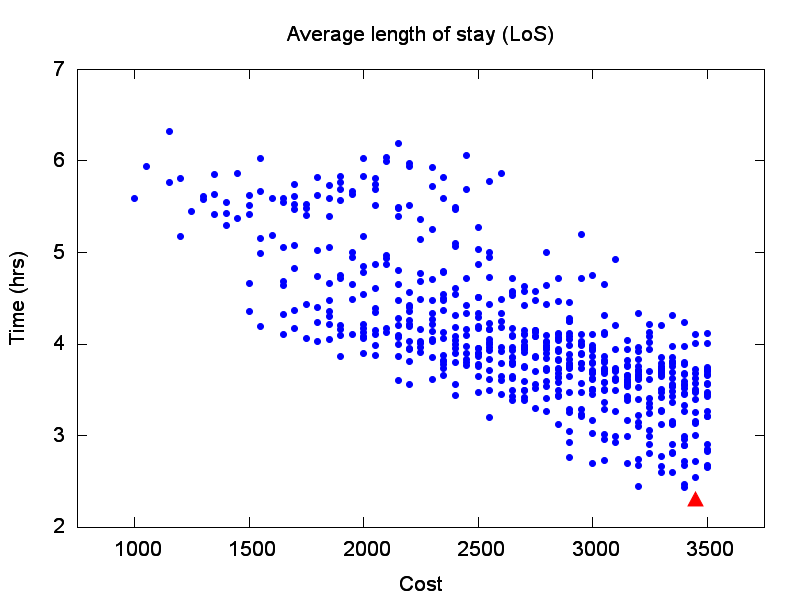
\includegraphics[width=1\columnwidth]{figs4/v0/6400-602-100-exh-LoS-min.png}
\par\end{center}

\vspace*{-1cm}

\noindent \begin{center}
\caption{Average LoS obtained by the ES method. The red triangle was the minimum.\label{subfig:es16}}

\par\end{center}%
\end{minipage}\hfill{}%
\begin{minipage}[t][1\totalheight][s]{0.48\linewidth}%
\noindent \begin{center}
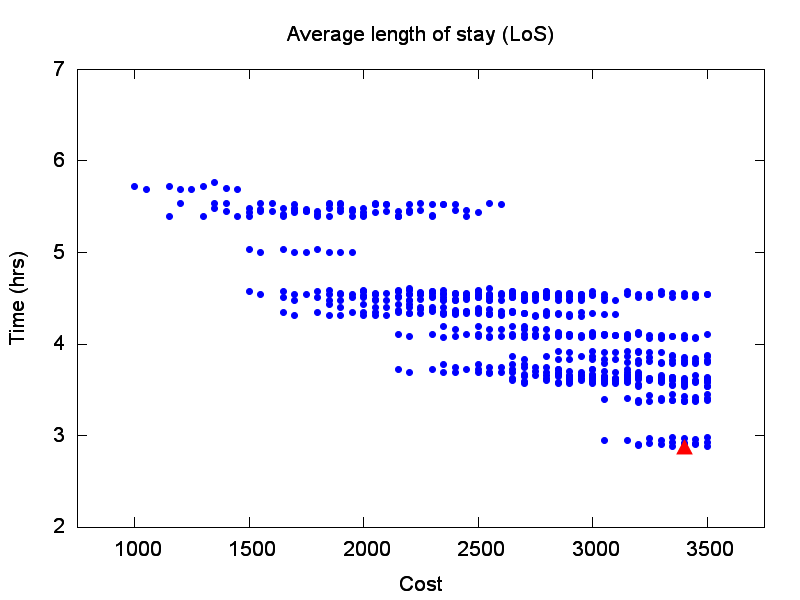
\includegraphics[width=1\columnwidth]{figs4/v0/pipe-sorted-LoS_1.0_min.png}
\par\end{center}

\vspace*{-1cm}

\noindent \begin{center}
\caption{Average LoS obtained by the PA. The red triangle was the maximum.\label{subfig:pipe16}}

\par\end{center}%
\end{minipage}
\par\end{centering}

\noindent \begin{centering}
%\centering\vspace{0cm}
\vspace*{-1.2cm}
\par\end{centering}

\begin{minipage}[t][1\totalheight][s]{0.48\textwidth}%
\noindent \begin{center}
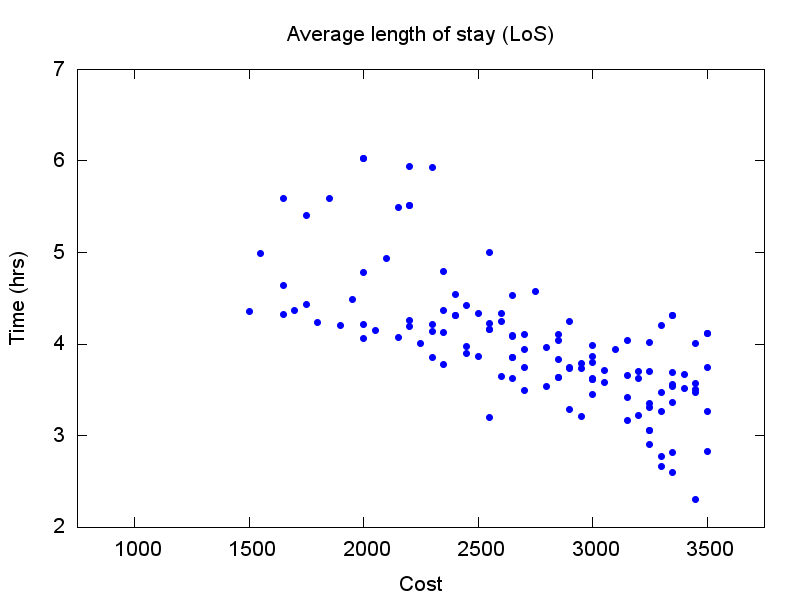
\includegraphics[width=1\columnwidth]{figs4/v0/MC/MC-6400-602-100-69-25-125confs-LoS.png}
\par\end{center}

\vspace*{-0.8cm}

\caption{Average LoS of 125 configurations obtained by the MC method. \label{subfig:mc16-1}}
%
\end{minipage}\hfill{}%
\begin{minipage}[t][1\totalheight][s]{0.48\textwidth}%
\noindent \begin{center}
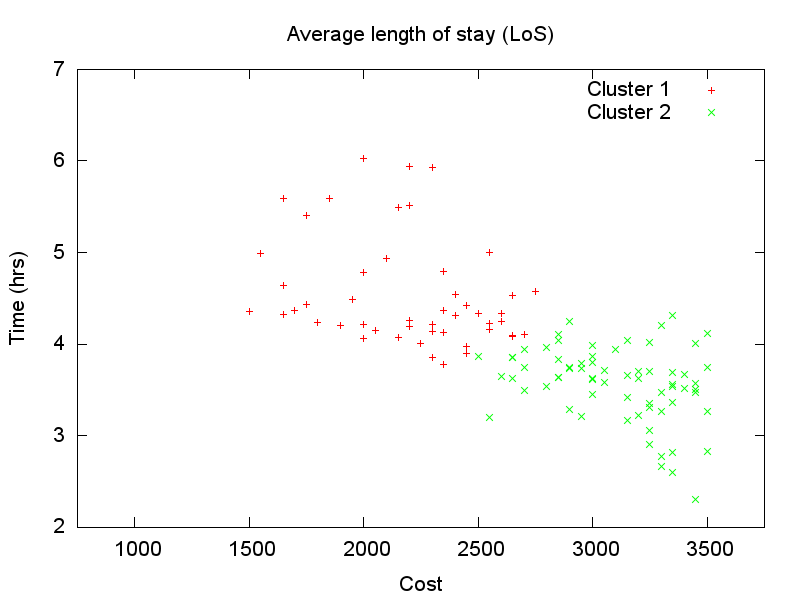
\includegraphics[width=1\columnwidth]{figs4/v0/MC/K-means-6400-602-100-69-25-125-Cluster1-49_Cluster2-68.png}
\par\end{center}

\vspace*{-0.8cm}

\caption{The K-means method identified two clusters of average number of attended
patients. The green one delimited the region where the minimum was.\label{subfig:km16-1}}
%
\end{minipage}

\vspace*{0.4cm}{\bf Figures} show the average LoS of the fourth workload scenario (17 patients/hour) using the ES, the PA, and the MC+K-means methods.
\end{figure}
\end{comment}
\begin{comment}
\begin{figure}[h]
\hfill{}\subfloat[\label{subfloat:pipe16} Scattered 3D graph of doctors, nurses, and
admission personnel.]{

\includegraphics[width=0.48\columnwidth]{figs4/6400-602-100-3D-scatter-LoS.png}}\hfill{}\subfloat[\label{subfloat:contour16} Contour graph where doctors and nurses
can be seen.]{

\includegraphics[width=0.48\columnwidth]{figs4/6400-602-100-sort-pipe_p5_y_p4-contour.png}}\hfill{}

\caption{\label{fig:Two-vision4} Graphs show the average LoS index of the
fourth workload scenario (17 patients/hour) using the first column
of \ref{subtab:As-pipe}, \ref{subtab:Ns-pipe}, and \ref{subtab:Ds-pipe},
where they were ordered by the pipeline approach (PA) \ref{eq:Pipeline formula}.
The colour bar is expresed in tics ( $hours\:=\frac{tics}{1000}$
). }
\end{figure}
\end{comment}
%\hspace{6cm}
%\vspace{-.5cm}


\begin{table}[h]
\caption{Optimum staff configurations that got the average minimum LoS for
this workload scenario (up to 17 patients hourly), where S is Senior
and J is Junior. This optimum sanitary staff configuration is shown
in red triangle in \ref{subfig:es17-1} and in black triangle in \ref{fig:3D-scattered-graph-100}.}


\begin{centering}
\begin{tabular}{cccccc>{\centering}p{2.8cm}}
\hline 
Method & euro & LoS (hrs) & D & N & A & Run time (hrs)

4 Pthreads\tabularnewline
\hline 
ES & 3,450  & 2.3  & 4J & 3J & 2S & 3.42\tabularnewline
PA & 3,450 & 2.3 & 4J & 3J & 2S & 0.15\tabularnewline
MC+K-means & 3,450  & 2.3  & 4J & 3J & 2S & 2.0\tabularnewline
\hline 
\end{tabular}
\par\end{centering}

\label{tab:16p-a} 
\end{table}


\begin{comment}
In the other cases, where the patient arrival increases there are
only few staff configurations around the minimum, or clearly only
one. But not only the patient arrival increases, but also the minimum
average patient stay time, as expected, but also the standard deviation,
patients at waiting rooms, both WR0 and WR1 at times t1, t2, t3, and
t4, and finally the amount of unattended patients increases too. In
\ref{tab:20_40_60_80_I1} all these results are shown. In Figure \ref{fig:exp1_WR}
the amount of patients in WR are shown, WR0 plus WR1, at four different
moments, t1=6,000, t2=12,000, t3=18,000, t4=24,000, during the simulation
for all the seven cases reported. It is noticed when the patient arrival
is high, 17 per hour, patients at waiting rooms increased.

%\hspace{6cm}
%\vspace{-.5cm}


\begin{table}[h]
\caption{Results for the best average minimum for each of the four presented
scenarios.}


{\small{\addtolength{\tabcolsep}{-5pt} }}{\small \par}

\begin{centering}
\resizebox{5.5in}{!}{{\small{}}%
\begin{tabular}{|c|c|c|c|c|c|c|c|}
\hline 
\multicolumn{1}{|c|}{{\small{P}}} & \multicolumn{1}{c|}{{\small{T1 }}} & \multicolumn{1}{c|}{{\small{ $\sigma$ }}} & \multicolumn{1}{c|}{{\small{Euros }}} & \multicolumn{1}{c|}{{\small{\# attended }}} & \multicolumn{1}{c|}{{\small{\# unattended }}} & {\small{WR0 }} & {\small{WR1 }}\tabularnewline
\cline{7-8} 
\multicolumn{1}{|c|}{} & \multicolumn{1}{c|}{} & \multicolumn{1}{c|}{} & \multicolumn{1}{c|}{} & \multicolumn{1}{c|}{{\small{patients}}} & \multicolumn{1}{c|}{{\small{patients}}} & {\small{t1, t2, t3, t4 }} & {\small{t1, t2, t3, t4 }}\tabularnewline
\hline 
{\small{4 }} & {\small{428 }} & {\small{48 (11\%) }} & {\small{2,850 }} & {\small{83 }} & {\small{1 }} & {\small{0,0,0,0 }} & {\small{0,0,0,0 }}\tabularnewline
\hline 
9 & {\small{514 }} & {\small{81.5 (15.9\%) }} & {\small{3,150 }} & {\small{182 }} & {\small{4 }} & {\small{0,0,0,1 }} & {\small{0,0,0,0 }}\tabularnewline
\hline 
{\small{13 }} & {\small{790 }} & {\small{174.5 (22.1\%) }} & {\small{3,400 }} & {\small{290 }} & {\small{8 }} & {\small{1,1,0,1 }} & {\small{3,2,4,1 }}\tabularnewline
\hline 
{\small{17 }} & {\small{3266 }} & {\small{1670.4 (51.2\%) }} & {\small{3,350 }} & {\small{294 }} & {\small{100 }} & {\small{8,19,32,43 }} & {\small{12,25,37,51 }}\tabularnewline
\hline 
\end{tabular}{\small{}}}
\par\end{centering}{\small \par}

{\small{\label{tab:20_40_60_80_I1}}}
\end{table}
\end{comment}
\clearpage{}


\subsection{Throughput Index}

The second objective set was to maximise number of attended patients
per day (Throughput) in the ED, with cost configuration constraint
less or equal to 3,500 euro. This index is expressed mathematically in
\ref{eq:Throughput index}:\vspace*{-0.125cm}
\begin{equation}
\begin{aligned} & {\text{Maximise patients attended}} &  & f(D,N,A)\\
 & \text{subject to} &  & D_{cost}+N_{cost}+A_{cost}\in Cost\leq3,500\:\text{euro}
\end{aligned}
\label{eq:Throughput index}
\end{equation}


It is worth noting that each of the plotted points were obtained running
the ED simulator as many times as points are. Each plotted point corresponds
to each of the 602 staff configurations (out of 1,134) that satisfy
the cost restriction.


\subsubsection{First Workload Scenario}

The results of this scenario, up to 4 patients/hour, are shown from
\ref{subfig:es4-2} to \ref{subfig:km4-2}. \ref{subfig:es4-2} shows
ES results. The red triangles were the maxima.
\begin{figure}[H]
\centering{}\vspace*{-0.2cm}\includegraphics[width=0.9\columnwidth,height=0.19\paperheight]{figs4/v0.2/6400-602-25-exh-throughput-max}\caption{Average number of attended patients obtained by the ES method. The
red triangles were the maxima. \label{subfig:es4-2}}
\end{figure}
 \vspace*{-0.2cm}

\begin{figure}[H]
\centering{}\vspace*{-0.2cm}\includegraphics[width=0.9\columnwidth,height=0.19\paperheight]{figs4/v0.2/pipe-sorted-Throughput_0_25_max}\caption{Average number of attended patients obtained by the PA. The red triangles
were the maxima. \label{subfig:pipe4-2}}
\end{figure}
 The PA result is shown in \ref{subfig:pipe4-2}, where three regions
can be clearly seen and the red triangles were the maxima. The most
important is the top region, in which the average maximum Throughput
was more than 80 attended patients. There were 440 configurations
(from a total of 602 in the feasible region) in this region, which
was the one where the maxima were.

The MC plus the K-means methods results are shown in \ref{subfig:mc4-2}
to \ref{subfig:km4-2}, respectively. The MC method found 50 configurations.
\begin{figure}[H]
\centering{}\vspace*{-0.2cm}\includegraphics[width=0.9\columnwidth,height=0.22\paperheight]{figs4/v0.2/MC/MC-6400-602-25-69-25-50confs-Throughput}\caption{Average number of attended patients of 50 configurations obtained
by the MC method.\label{subfig:mc4-2}}
\end{figure}
However, it was difficult to get any conclusion about such region;
therefore, the complementary K-means method was performed. The K-means
method identified two different clusters, shown in \ref{subfig:km4-2}.
The most important was the green cluster, which delimited the region
where the optima were.
\begin{figure}[H]
\begin{centering}
\vspace*{-0.2cm}\includegraphics[width=0.9\columnwidth,height=0.22\paperheight]{figs4/v0.2/MC/K-means-6400-602-25-69-25-50-Cluster1-23_Cluster2-25}
\par\end{centering}

\caption{The K-means method identified two clusters of average number of attended
patients. The green one delimited the region where the maxima were.\label{subfig:km4-2}}
\end{figure}


\begin{comment}
The graphics \ref{subfloat:pipe4} and \ref{subfloat:contour4} shown
another way to visualise the connectivity characteristic of the reduced
regions found by the AP, and the MC plus the K-means methods. In such
connected reduced regions the ``reduced exhaustive search'' is applied.
The axes of such graphs are the first column of \ref{subtab:As-pipe},
\ref{subtab:Ns-pipe}, and \ref{subtab:Ds-pipe}, where they were
ordered by the pipeline approach (PA) \ref{eq:Pipeline formula}.
\end{comment}


Finally, after separately applied both the PA and the MC plus the
K-means methods, the \textquotedblleft{}reduced exhaustive search\textquotedblright{}
was separately performed in each reduced region identified. The optimum
found per each method: the ES, the PA, and the MC plus the K-means
methods are presented in \ref{tab:4p-b}, where the sanitary staff
configuration (doctors, nurses, and admission personnel), their associated
average maximum Throughput, and cost configuration are shown. The
three optima independently found were the same. 
\begin{table}[H]
\caption{Optimum staff configurations that got the average maximum Throughput
for this workload scenario (up to 4 patients hourly), where S is Senior
and J is Junior. These optimum sanitary staff configurations are shown
in red triangle in \ref{subfig:es4-2}.}


\begin{centering}
\begin{tabular}{cc>{\centering}p{2cm}ccc>{\centering}p{2.8cm}}
\hline 
Method & euro & \#attended patients & D & N & A & Run time (hrs)

4 Pthreads\tabularnewline
\hline 
ES & 3,050 & 86 & 2S & 1S,1J & 1S & 0.91\tabularnewline
PA & 3,050 & 86 & 2S & 1S,1J & 1S & 0.63\tabularnewline
MC+K-means & 3,050 & 86 & 2S & 1S,1J & 1S & 0.73\tabularnewline
\hline 
\end{tabular}
\par\end{centering}

\label{tab:4p-b} 
\end{table}


\begin{comment}
The results are shown in the Figure \ref{fig:exp2_80}, where the
blue points are the staff configuration that satisfy the restriction,
while the red point is the minimum. Its configuration is presented
in Table \ref{2o_I_80_20}. It order to get the same time or less,
the superior limit for staff members was increased to: $doctors<9$;
$nurses<7$, and $admissions<5$. This index can be seen as looking
for a staff configuration that guarantee, at least, the same quality
for high patient arrival, 17 per hour, as the same that was gotten
for low patient arrival, 4 per hour.
\end{comment}
\begin{comment}
\begin{figure}[h]
\noindent \begin{centering}
\begin{minipage}[t][1\totalheight][s]{0.48\columnwidth}%
\noindent \begin{center}
\includegraphics[width=1\columnwidth]{figs4/v0.2/6400-602-25-exh-throughput-max.png}
\par\end{center}

\vspace*{-1cm}

\noindent \begin{center}
\caption{Average number of attended patients obtained by the ES method. The
red triangles were the maximum. }

\par\end{center}%
\end{minipage}\hfill{}%
\begin{minipage}[t][1\totalheight][s]{0.48\columnwidth}%
\noindent \begin{center}
\includegraphics[width=1\columnwidth]{figs4/v0.2/pipe-sorted-Throughput_0.25_max.png}
\par\end{center}

\vspace*{-1cm}

\noindent \begin{center}
\caption{Average number of attended patients obtained by the PA. The red triangles
were the maximum. }

\par\end{center}%
\end{minipage}
\par\end{centering}

\noindent \begin{centering}
%\centering\vspace{0cm}
\vspace*{-1.2cm}
\par\end{centering}

\begin{minipage}[t][1\totalheight][s]{0.48\columnwidth}%
\noindent \begin{center}
\includegraphics[width=1\columnwidth]{figs4/v0.2/MC/MC-6400-602-25-69-25-50confs-Throughput-TRI.pdf}
\par\end{center}

\vspace*{-0.8cm}

\caption{Average number of attended patients of 50 configurations obtained
by the MC method. }
%
\end{minipage}\hfill{}%
\begin{minipage}[t][1\totalheight][s]{0.48\columnwidth}%
\noindent \begin{center}
\includegraphics[width=1\columnwidth]{figs4/v0.2/MC/K-means-6400-602-25-69-25-50-Cluster1-23_Cluster2-25_TRI.pdf}
\par\end{center}

\vspace*{-0.8cm}

\caption{The K-means method identified two clusters of average number of attended
patients. The green one delimited the region where the maximum were.}
%
\end{minipage}

\vspace*{0.4cm}{\bf Figures} show the average Throughput of the first workload scenario (4 patients/hour) using the ES, the PA, and the MC+K-means methods.
\end{figure}
\end{comment}


\begin{comment}
From Figures \ref{fig:exp1_20} and \ref{tab:4p-b}, there is a staff
configuration that got the minimum time. Also, in such Figures \ref{fig:exp1_20}
can appreciate that there are many other staff configurations that
are quite close to the optimum, but with less cost.
\end{comment}



\subsubsection{Second Workload Scenario}

The results of this scenario, up to 9 patients/hour, are shown from
\ref{subfig:es8-2} to \ref{subfig:km8-2}. The ES result is shown
in \ref{subfig:es8-2}, where the red triangle was the maximum. 
\begin{figure}[H]
\centering{}\includegraphics[width=0.95\columnwidth,height=0.25\paperheight]{figs4/v0.2/6400-602-50-exh-throughput-max}\caption{Average number of attended patients obtained by the ES method. The
red triangle was the maximum.\label{subfig:es8-2}}
\end{figure}


The PA result is shown in \ref{subfig:pipe8-2}, where many regions
can be seen and the red triangle was the maximum. 
\begin{figure}[H]
\centering{}\includegraphics[width=0.95\columnwidth,height=0.25\paperheight]{figs4/v0.2/pipe-sorted-Throughput_0_50_max}\caption{Average number of attended patients obtained by the PA. The red triangles
were the maximum.\label{subfig:pipe8-2}}
\end{figure}
 The most important is the top region, in which the average maximum
Throughput was more than 150 attended patients. There were 180 configurations
(from a total of 602 in the feasible region) in this region, which
was the one where the maximum was.

The MC plus the K-means methods results are shown in \ref{subfig:mc8-2}
to \ref{subfig:km8-2}, respectively. The MC method found 125 configurations.
\begin{figure}[H]
\centering{}\includegraphics[width=0.95\columnwidth,height=0.25\paperheight]{figs4/v0.2/MC/MC-6400-602-50-69-25-125confs-Throughput}\caption{Average number of attended patients of 125 configurations obtained
by the MC method. \label{subfig:mc8-2}}
\end{figure}
 However, it was difficult to get any conclusion about such region;
therefore, the complementary K-means method was performed. The K-means
method identified two different clusters, shown in \ref{subfig:km8-2}.
The most important was the green cluster, which delimited the region
where the optimum was.
\begin{figure}[H]
\begin{centering}
\includegraphics[width=0.95\columnwidth,height=0.25\paperheight]{figs4/v0.2/MC/K-means-6400-602-50-69-25-125-Cluster1-56_Cluster2-60}
\par\end{centering}

\caption{The K-means method identified two clusters of average number of attended
patients. The green one delimited the region where the maximum was.\label{subfig:km8-2}}
\end{figure}


\begin{comment}
The graphics \ref{subfloat:pipe4} and \ref{subfloat:contour4} shown
another way to visualise the connectivity characteristic of the reduced
regions found by the AP, and the MC plus the K-means methods. In such
connected reduced regions the ``reduced exhaustive search'' is applied.
The axes of such graphs are the first column of \ref{subtab:As-pipe},
\ref{subtab:Ns-pipe}, and \ref{subtab:Ds-pipe}, where they were
ordered by the pipeline approach (PA) \ref{eq:Pipeline formula}.
\end{comment}


Finally, after separately applied both the PA and the MC plus the
K-means methods, the \textquotedblleft{}reduced exhaustive search\textquotedblright{}
was separately performed in each reduced region identified. The optimum
found per each method: the ES, the PA, and the MC plus the K-means
methods are presented in \ref{tab:8p-b}, where the sanitary staff
configuration (doctors, nurses, and admission personnel), their associated
average maximum Throughput, and cost configuration are shown. The
three optima independently found were the same.

\begin{comment}
\begin{figure}[h]
\noindent \begin{centering}
\begin{minipage}[t][1\totalheight][s]{0.48\columnwidth}%
\noindent \begin{center}
\includegraphics[width=1\columnwidth]{figs4/v0.2/6400-602-50-exh-throughput-max.png}
\par\end{center}

\vspace*{-1cm}

\noindent \begin{center}
\caption{}

\par\end{center}%
\end{minipage}\hfill{}%
\begin{minipage}[t][1\totalheight][s]{0.48\columnwidth}%
\noindent \begin{center}
\includegraphics[width=1\columnwidth]{figs4/v0.2/pipe-sorted-Throughput_0.50_max.png}
\par\end{center}

\vspace*{-1cm}

\noindent \begin{center}
\caption{}

\par\end{center}%
\end{minipage}
\par\end{centering}

\noindent \begin{centering}
%\centering\vspace{0cm}
\vspace*{-1.2cm}
\par\end{centering}

\begin{minipage}[t][1\totalheight][s]{0.48\columnwidth}%
\noindent \begin{center}
\includegraphics[width=1\columnwidth]{figs4/v0.2/MC/MC-6400-602-50-69-25-125confs-Throughput.png}
\par\end{center}

\vspace*{-0.8cm}

\caption{}
%
\end{minipage}\hfill{}%
\begin{minipage}[t][1\totalheight][s]{0.48\columnwidth}%
\noindent \begin{center}
\includegraphics[width=1\columnwidth]{figs4/v0.2/MC/K-means-6400-602-50-69-25-125-Cluster1-56_Cluster2-60.png}
\par\end{center}

\vspace*{-0.8cm}

\caption{}
%
\end{minipage}

\vspace*{0.4cm}{\bf Figures} show the average Throughput of the second workload scenario (9 patients/hour) using the ES, the PA, and the MC+K-means methods.
\end{figure}
\end{comment}


\begin{table}[H]
\caption{Optimum staff configurations that got the average maximum Throughput
for this workload scenario (up to 9 patients hourly), where S is Senior
and J is Junior. These optimum sanitary staff configurations are shown
in red triangle in \ref{subfig:es8-2}.}


\begin{centering}
\begin{tabular}{cc>{\centering}p{2cm}ccc>{\centering}p{2.8cm}}
\hline 
Method & euro & \#attended patients & D & N & A & Run time (hrs)

4 Pthreads\tabularnewline
\hline 
ES & 3,350 & 163 & 1S,2J & 2S & 1S,1J & 1.59\tabularnewline
PA & 3,350 & 163 & 1S,2J & 2S & 1S,1J & 0.39\tabularnewline
MC+K-means & 3,350 & 163 & 1S,2J & 2S & 1S,1J & 1.08\tabularnewline
\hline 
\end{tabular}
\par\end{centering}

\label{tab:8p-b} 
\end{table}



\subsubsection{Third Workload Scenario}

The results of this scenario, up to 13 patients/hour, are shown from
\ref{subfig:es12-2} to \ref{subfig:km12-2}. The ES result is shown
in \ref{subfig:es12-2}, where the red triangle was the maximum. 

The PA result is shown in \ref{subfig:pipe12-2}, many regions can
be seen and the red triangle was the maximum. The most important is
the top region, in which the average maximum Throughput was more than
200 attended patients. There were 21 configurations (from a total
of 602 in the feasible region) in this region, which is the one where
the maximum was.

\begin{figure}[H]
\centering{}\includegraphics[width=0.95\columnwidth,height=0.25\paperheight]{figs4/v0.2/6400-602-75-exh-throughput-max}\caption{Average number of attended patients obtained by the ES method. The
red triangle was the maximum. \label{subfig:es12-2}}
\end{figure}
 
\begin{figure}[H]
\centering{}\includegraphics[width=0.95\columnwidth,height=0.25\paperheight]{figs4/v0.2/pipe-sorted-Throughput_0_75_max}\caption{Average number of attended patients obtained by the PA. The red triangles
were the maximum.\label{subfig:pipe12-2}}
\end{figure}


The MC plus the K-means methods results are shown in \ref{subfig:mc12-2}
to \ref{subfig:km12-2}, respectively. The MC method found 275 configurations.
\begin{figure}[H]
\centering{}\includegraphics[width=0.95\columnwidth,height=0.25\paperheight]{figs4/v0.2/MC/MC-6400-602-75-69-25-275confs-Throughput}\caption{Average number of attended patients of 275 configurations obtained
by the MC method. \label{subfig:mc12-2}}
\end{figure}
 However, it was difficult to get any conclusion about such region;
therefore, the complementary K-means method was performed. The K-means
method identified two different clusters, shown in \ref{subfig:km12-2},
the most important was the green cluster, which delimited the region
where the optimum was.
\begin{figure}[H]
\begin{centering}
\includegraphics[width=0.95\columnwidth,height=0.25\paperheight]{figs4/v0.2/MC/K-means-6400-602-75-69-25-275-Cluster1-91_Cluster2-123}
\par\end{centering}

\caption{The K-means method identified two clusters of average number of attended
patients. The green one delimited the region where the maximum was.\label{subfig:km12-2}}
\end{figure}


\begin{comment}
The graphics \ref{subfloat:pipe4} and \ref{subfloat:contour4} shown
another way to visualise the connectivity characteristic of the reduced
regions found by the AP, and the MC plus the K-means methods. In such
connected reduced regions the ``reduced exhaustive search'' is applied.
The axes of such graphs are the first column of \ref{subtab:As-pipe},
\ref{subtab:Ns-pipe}, and \ref{subtab:Ds-pipe}, where they were
ordered by the pipeline approach (PA) \ref{eq:Pipeline formula}.
\end{comment}


Finally, after separately applied both the PA and the MC plus the
K-means methods, the \textquotedblleft{}reduced exhaustive search\textquotedblright{}
was separately performed in each reduced region identified. The optimum
found per each method: the ES, the PA, and the MC plus the K-means
methods are presented in \ref{tab:12p-b}, where the sanitary staff
configuration (doctors, nurses, and admission personnel), and their
associated average maximum Throughput, and cost configuration are
shown. The three optima independently found were the same.

\begin{comment}
\begin{figure}[h]
\noindent \begin{centering}
\begin{minipage}[t][1\totalheight][s]{0.48\columnwidth}%
\noindent \begin{center}
\includegraphics[width=1\columnwidth]{figs4/v0.2/6400-602-75-exh-throughput-max.png}
\par\end{center}

\vspace*{-1cm}

\noindent \begin{center}
\caption{}

\par\end{center}%
\end{minipage}\hfill{}%
\begin{minipage}[t][1\totalheight][s]{0.48\columnwidth}%
\noindent \begin{center}
\includegraphics[width=1\columnwidth]{figs4/v0.2/pipe-sorted-Throughput_0.75_max.png}
\par\end{center}

\vspace*{-1cm}

\noindent \begin{center}
\caption{}

\par\end{center}%
\end{minipage}
\par\end{centering}

\noindent \begin{centering}
%\centering\vspace{0cm}
\vspace*{-1.2cm}
\par\end{centering}

\begin{minipage}[t][1\totalheight][s]{0.48\columnwidth}%
\noindent \begin{center}
\includegraphics[width=1\columnwidth]{figs4/v0.2/MC/MC-6400-602-75-69-25-275confs-Throughput.png}
\par\end{center}

\vspace*{-0.8cm}

\caption{}
%
\end{minipage}\hfill{}%
\begin{minipage}[t][1\totalheight][s]{0.48\columnwidth}%
\noindent \begin{center}
\includegraphics[width=1\columnwidth]{figs4/v0.2/MC/K-means-6400-602-75-69-25-275-Cluster1-91_Cluster2-123.png}
\par\end{center}

\vspace*{-0.8cm}

\caption{}
%
\end{minipage}

\vspace*{0.4cm}{\bf Figures} show the average Throughput of the third workload scenario (13 patients/hour) using the ES, the PA, and the MC+K-means methods.
\end{figure}
\end{comment}


\begin{table}[H]
\caption{Optimum staff configurations that got the average maximum Throughput
for this workload scenario (up to 13 patients hourly), where S is
Senior and J is Junior. This optimum sanitary staff configuration
is shown in red triangle in \ref{subfig:es12-2}.}


\begin{centering}
\begin{tabular}{cc>{\centering}p{2cm}ccc>{\centering}p{2.8cm}}
\hline 
Method & euro & \#attended patients & D & N & A & Run time (hrs)

4 Pthreads\tabularnewline
\hline 
ES & 3,200 & 205 & 4J & 2S & 1S & 2.46\tabularnewline
PA & 3,200 & 205 & 4J & 2S & 1S & 0.13\tabularnewline
MC+K-means & 3,200 & 205 & 4J & 2S & 1S & 1.51\tabularnewline
\hline 
\end{tabular}
\par\end{centering}

\label{tab:12p-b}
\end{table}



\subsubsection{Fourth Workload Scenario}

The results of this scenario, up to 17 patients/hour, are shown from
\ref{subfig:es16-2} to \ref{subfig:km16-2}. The ES result is shown
in \ref{subfig:es16-2}, where the red triangle was the maximum. 
\begin{figure}[H]
\centering{}\includegraphics[width=0.95\columnwidth,height=0.25\paperheight]{figs4/v0.2/6400-602-100-exh-throughput-max}\caption{Average number of attended patients obtained by the ES method. The
red triangle was the maximum.\label{subfig:es16-2}}
\end{figure}


The PA result is shown in \ref{subfig:pipe16-2}, many regions can
be seen and the red triangle was the maximum. The most important is
the top region, in which the average maximum Throughput was more than
200 attended patients. There were 21 configurations (from a total
of 602 in the feasible region) in this region, which is the one where
the maximum was.
\begin{figure}[H]
\centering{}\includegraphics[width=0.95\columnwidth,height=0.25\paperheight]{figs4/v0.2/pipe-sorted-Throughput_1_0_max}\caption{Average number of attended patients obtained by the PA. The red triangles
were the maximum.\label{subfig:pipe16-2}}
\end{figure}


The MC plus the K-means methods results are shown in \ref{subfig:mc16-2}
to \ref{subfig:km16-2}, respectively. The MC method found 125 configurations.
\begin{figure}[H]
\centering{}\includegraphics[width=0.95\columnwidth,height=0.25\paperheight]{figs4/v0.2/MC/MC-6400-602-100-69-25-125confs-Throughput}\caption{Average number of attended patients of 125 configurations obtained
by the MC method. \label{subfig:mc16-2}}
\end{figure}
However, it was difficult to get any conclusion about such region;
therefore, the complementary K-means method was performed. The K-means
method identified two different clusters, shown in \ref{subfig:km16-2},
the most important was the green cluster, which delimited the region
where the optimum was.
\begin{figure}[H]
\begin{centering}
\includegraphics[width=0.95\columnwidth,height=0.25\paperheight]{figs4/v0.2/MC/K-means-6400-602-100-69-25-125-Cluster1-56_Cluster2-60}
\par\end{centering}

\caption{The K-means method identified two clusters of average number of attended
patients. The green one delimited the region where the maximum was.\label{subfig:km16-2}}
\end{figure}


\begin{comment}
The graphics \ref{subfloat:pipe4} and \ref{subfloat:contour4} shown
another way to visualise the connectivity characteristic of the reduced
regions found by the AP, and the MC plus the K-means methods. In such
connected reduced regions the ``reduced exhaustive search'' is applied.
The axes of such graphs are the first column of \ref{subtab:As-pipe},
\ref{subtab:Ns-pipe}, and \ref{subtab:Ds-pipe}, where they were
ordered by the pipeline approach (PA) \ref{eq:Pipeline formula}.
\end{comment}


Finally, after separately applied both the PA and the MC plus the
K-means methods, the \textquotedblleft{}reduced exhaustive search\textquotedblright{}
was separately performed in each reduced region identified. The optimum
found per each method: the ES, the PA, and the MC plus the K-means
methods are presented in \ref{tab:16p-b}, where the sanitary staff
configuration (doctors, nurses, and admission personnel), their associated
average maximum Throughput, and cost configuration are shown. The
three optima independently found were the same.

\begin{comment}
\begin{figure}[h]
\noindent \begin{centering}
\begin{minipage}[t][1\totalheight][s]{0.48\linewidth}%
\noindent \begin{center}
\includegraphics[width=1\columnwidth]{figs4/v0.2/6400-602-100-exh-throughput-max.png}
\par\end{center}

\vspace*{-1cm}

\noindent \begin{center}
\caption{}

\par\end{center}%
\end{minipage}\hfill{}%
\begin{minipage}[t][1\totalheight][s]{0.48\linewidth}%
\noindent \begin{center}
\includegraphics[width=1\columnwidth]{figs4/v0.2/pipe-sorted-Throughput_1.0_max.png}
\par\end{center}

\vspace*{-1cm}

\noindent \begin{center}
\caption{}

\par\end{center}%
\end{minipage}
\par\end{centering}

\noindent \begin{centering}
%\centering\vspace{0cm}
\vspace*{-1.2cm}
\par\end{centering}

\begin{minipage}[t][1\totalheight][s]{0.48\textwidth}%
\noindent \begin{center}
\includegraphics[width=1\columnwidth]{figs4/v0.2/MC/MC-6400-602-100-69-25-125confs-Throughput.png}
\par\end{center}

\vspace*{-0.8cm}

\caption{}
%
\end{minipage}\hfill{}%
\begin{minipage}[t][1\totalheight][s]{0.48\textwidth}%
\noindent \begin{center}
\includegraphics[width=1\columnwidth]{figs4/v0.2/MC/K-means-6400-602-100-69-25-125-Cluster1-56_Cluster2-60.png}
\par\end{center}

\vspace*{-0.8cm}

\caption{}
%
\end{minipage}

\vspace*{0.4cm}{\bf Figures} show the average Throughput of the fourth workload scenario (17 patients/hour) using the ES, the PA, and the MC+K-means methods.
\end{figure}
\end{comment}


\begin{table}[h]
\caption{Optimum staff configurations that got the average maximum Throughput
for this workload scenario (up to 17 patients hourly), where S is
Senior and J is Junior. This optimum sanitary staff configuration
is shown in red triangle in \ref{subfig:es16-2}.}


\begin{centering}
\begin{tabular}{cc>{\centering}p{2cm}ccc>{\centering}p{2.8cm}}
\hline 
Method & euro & \#attended patients & D & N & A & Run time (hrs)

4 Pthreads\tabularnewline
\hline 
ES & 3,400 & 221 & 4J & 3J & 1S,1J & 3.43\tabularnewline
PA & 3,400 & 221 & 4J & 3J & 1S,1J & 0.10\tabularnewline
MC+K-means & 3,400 & 221 & 4J & 3J & 1S,1J & 2.06\tabularnewline
\hline 
\end{tabular}
\par\end{centering}

\label{tab:16p-b} 
\end{table}



\subsection{CLoS Index}

The third objective set was to minimise a compound index: $Cost\times LoS$,
(CLoS), without any restriction, except the minimum and maximum number
of admission personnel, nurses, and doctors stated in \ref{subtab:As}
to \ref{subtab:Ds}. This index is expressed mathematically in \ref{eq:CLoS index}:

\begin{equation}
\begin{aligned} & {\text{Minimise }CLoS} &  & f(D,N,A)\end{aligned}
\label{eq:CLoS index}
\end{equation}


As a consequence of not having any constraint, 1,134 ($14D*9N*9A$)
staff configurations, that represent the whole search space, were
tested for each of the four workload scenarios of incoming patients
stated in \ref{tab:scenarios}. Each of the plotted points were obtained
running the ED simulator as many times those points are, 1,134.


\subsubsection{First Workload Scenario}

The results of this scenario, up to 4 patients/hour, are shown from
\ref{subfig:es4-3} to \ref{subfig:km4-3}. The 3D scattered graphics
shown the average minimum CLoS index by its colour. 
\begin{figure}[H]
\centering{}\includegraphics[width=1\columnwidth,height=0.2\paperheight]{figs4/v0.3/6400-602-25-Cost_times_LoS-exh-min}\caption{Average CLoS obtained by the ES method. The black triangle was the
minimum. CLoS units are in thousands. \label{subfig:es4-3}}
\end{figure}
The green colour represents the value in the vicinity of the optimum,
the lighter green colours were the most relevant. The ES result is
shown in \ref{subfig:es4-3}, where the black triangle was the minimum. 

\begin{figure}[H]
\centering{}\includegraphics[width=1\columnwidth,height=0.2\paperheight]{figs4/v0.3/pipe-sorted-0.25-Cost_times_LoS_min}\caption{Average CLoS obtained by the PA. The black triangle was the minimum.
CLoS units are in thousands.\label{subfig:pipe4-3}}
\end{figure}
The PA result is shown in \ref{subfig:pipe4-3}, where the black triangle
was the minimum. Several regions can be seen. The most important was
where the black triangle was. There were 316 configurations (from
a total of 1,134) in this region, which is the one where the minimum
was.

The MC plus the K-means methods results are shown in \ref{subfig:mc4-3}
to \ref{subfig:km4-3}, respectively. The MC method found 75 configurations.
\begin{figure}[H]
\centering{}\includegraphics[width=1\columnwidth,height=0.2\paperheight]{figs4/v0.3/MC/MC-25-69-25-75-Cost_times_LoS}\caption{Average CLoS of 75 configurations obtained by the MC method. CLoS
units are in thousands. \label{subfig:mc4-3}}
\end{figure}
However, it was difficult to get any conclusion about such region;
therefore, the complementary K-means method was performed. The K-means
method identified two different clusters, shown in \ref{subfig:km4-3},
the most important was the red cluster, which delimited the region
where the optimum was. %
\begin{comment}
The graphics \ref{subfloat:pipe4} and \ref{subfloat:contour4} shown
another way to visualise the connectivity characteristic of the reduced
regions found by the AP, and the MC plus the K-means methods. In such
connected reduced regions the ``reduced exhaustive search'' is applied.
The axes of such graphs are the first column of \ref{subtab:As-pipe},
\ref{subtab:Ns-pipe}, and \ref{subtab:Ds-pipe}, where they were
ordered by the pipeline approach (PA) \ref{eq:Pipeline formula}.
\end{comment}
\begin{figure}[H]
\begin{centering}
\includegraphics[width=1\columnwidth,height=0.2\paperheight]{figs4/v0\lyxdot 3/MC/K-means-1134-25-69-25-75-Cluster1-67_Cluster2-7}
\par\end{centering}

\caption{The K-means method identified two clusters of average CLoS. The red
one delimited the region where the minimum was. \label{subfig:km4-3}}
\end{figure}


Finally, after separately applied both the PA and the MC plus the
K-means methods, the \textquotedblleft{}reduced exhaustive search\textquotedblright{}
was separately performed in each reduced region identified. The optimum
found per each method: the ES, the PA, and the MC plus the K-means
methods are presented in \ref{tab:4p-c}, where the sanitary staff
configuration (doctors, nurses, and admission personnel), their associated
average minimum CLoS, and cost configuration are shown. The three
optima independently found were the same. %
\begin{comment}
\begin{figure}[h]
\noindent \begin{centering}
\begin{minipage}[t]{0.45\linewidth}%
\noindent \begin{center}
\includegraphics[width=1\columnwidth]{figs4/v0.3/6400-602-25-Cost_times_LoS-exh-min.png}
\par\end{center}

\noindent \begin{center}
\caption{}

\par\end{center}%
\end{minipage}\hfill{}%
\begin{minipage}[t]{0.45\linewidth}%
\noindent \begin{center}
\includegraphics[width=1\columnwidth]{figs4/v0.3/pipe-sorted-0.25-Cost_times_LoS_min.png}
\par\end{center}

\noindent \begin{center}
\caption{}

\par\end{center}%
\end{minipage}
\par\end{centering}

\noindent \begin{centering}
\vfill{}

\par\end{centering}

\begin{minipage}[t]{0.45\textwidth}%
\noindent \begin{center}
\includegraphics[width=1\columnwidth]{figs4/v0.3/MC/MC-25-69-25-75-Cost_times_LoS.png}
\par\end{center}

\caption{}
%
\end{minipage}\hfill{}%
\begin{minipage}[t]{0.45\textwidth}%
\noindent \begin{center}
\includegraphics[width=1\columnwidth]{figs4/v0.3/MC/K-means-1134-25-69-25-75-Cluster1-67_Cluster2-7.png}
\par\end{center}

\caption{}
%
\end{minipage}
\end{figure}
\end{comment}
{} 

\begin{table}[H]
\caption{Optimum staff configurations that got the average minimum CLoS for
this workload scenario (up to 4 patients hourly), where S is Senior
and J is Junior. This optimum sanitary staff configuration is shown
in black triangle in \ref{subfig:es4-3}.}


\begin{centering}
\begin{tabular}{cccccc>{\centering}p{2.8cm}}
\hline 
Method & euro & CLoS & D & N & A & Run time (hrs)

32 Pthreads\tabularnewline
\hline 
ES & 1,500  & $1.03{}^{6}$ & 2J & 1J & 1J & 0.46\tabularnewline
PA & 1,500 & $1.03{}^{6}$ & 2J & 1J & 1J & 0.13\tabularnewline
MC+K-means & 1,500 & $1.03{}^{6}$ & 2J & 1J & 1J & 0.35\tabularnewline
\hline 
\end{tabular}
\par\end{centering}

\label{tab:4p-c} 
\end{table}



\subsubsection{Second Workload Scenario}

The results of this scenario, up to 9 patients/hour, are shown from
\ref{subfig:es8-3} to \ref{subfig:km8-3}. The 3D scattered graphics
shown the average minimum CLoS index by its colour. The green colour
represents the value in the vicinity of the optimum. The ES result
is shown in \ref{subfig:es8-3}, where the black triangle was the
minimum. 
\begin{figure}[H]
\centering{}\includegraphics[width=1\columnwidth,height=0.19\paperheight]{figs4/v0.3/6400-602-50-Cost_times_LoS-exh-min}\caption{Average CLoS obtained by the ES method. The black triangle was the
minimum. CLoS units are in thousands.\label{subfig:es8-3}}
\end{figure}


The PA result is shown in \ref{subfig:pipe8-3}, where the black triangle
was the minimum. Several regions can be seen. The most important was
where the black triangle was. There were 429 configurations (from
a total of 1,134) in this region, which is the one where the minimum
was.

The MC plus the K-means methods results are shown in \ref{subfig:mc8-3}
to \ref{subfig:km8-3}, respectively. The MC method found 275 configurations.
However, it was difficult to get any conclusion about such region;
therefore, the complementary K-means method was performed.
\begin{figure}[H]
\centering{}\includegraphics[width=1\columnwidth,height=0.19\paperheight]{figs4/v0.3/pipe-sorted-0.50-Cost_times_LoS_min}\caption{Average CLoS obtained by the PA. The black triangle was the minimum.
CLoS units are in thousands. \label{subfig:pipe8-3} }
\end{figure}
The K-means method identified three different clusters, shown in \ref{subfig:km8-3}.
\begin{figure}[H]
\centering{}\includegraphics[width=1\columnwidth,height=0.19\paperheight]{figs4/v0.3/MC/MC-50-69-25-275-Cost_times_LoS}\caption{CLoS of 275 configurations obtained by the MC method. CLoS units are
in thousands. \label{subfig:mc8-3}}
\end{figure}
\begin{figure}[H]
\begin{centering}
\includegraphics[width=1\columnwidth,height=0.19\paperheight]{figs4/v0.3/MC/K-means-1134-50-69-25-275-Cluster1-116_Cluster2-38-Cluster3-94}
\par\end{centering}

\caption{The K-means method identified three clusters of average CLoS. The
red one delimited the region where the minimum was. \label{subfig:km8-3}}
\end{figure}
 The most important cluster was the red one, which delimited the region
where the optimum was. 

\begin{comment}
The graphics \ref{subfloat:pipe4} and \ref{subfloat:contour4} shown
another way to visualise the connectivity characteristic of the reduced
regions found by the AP, and the MC plus the K-means methods. In such
connected reduced regions the ``reduced exhaustive search'' is applied.
The axes of such graphs are the first column of \ref{subtab:As-pipe},
\ref{subtab:Ns-pipe}, and \ref{subtab:Ds-pipe}, where they were
ordered by the pipeline approach (PA) \ref{eq:Pipeline formula}.
\end{comment}


Finally, after separately applied both the PA and the MC plus the
K-means methods, the \textquotedblleft{}reduced exhaustive search\textquotedblright{}
was separately performed in each reduced region identified. The optimum
found per each method: the ES, the PA, and the MC plus the K-means
methods are presented in \ref{tab:8p-c}, where the sanitary staff
configuration (doctors, nurses, and admission personnel), their associated
average minimum CLoS, and cost configuration are shown. The three
optima independently found were the same.

\begin{comment}
\begin{figure}[h]
\noindent \begin{centering}
\begin{minipage}[t]{0.45\linewidth}%
\noindent \begin{center}
\includegraphics[width=1\columnwidth]{figs4/v0.3/6400-602-50-Cost_times_LoS-exh-min.png}
\par\end{center}

\noindent \begin{center}
\caption{}

\par\end{center}%
\end{minipage}\hfill{}%
\begin{minipage}[t]{0.45\linewidth}%
\noindent \begin{center}
\includegraphics[width=1\columnwidth]{figs4/v0.3/pipe-sorted-0.50-Cost_times_LoS_min.png}
\par\end{center}

\noindent \begin{center}
\caption{}

\par\end{center}%
\end{minipage}
\par\end{centering}

\noindent \begin{centering}
\vfill{}

\par\end{centering}

\begin{minipage}[t]{0.45\textwidth}%
\noindent \begin{center}
\includegraphics[width=1\columnwidth]{figs4/v0.3/MC/MC-50-69-25-275-Cost_times_LoS.png}
\par\end{center}

\caption{}
%
\end{minipage}\hfill{}%
\begin{minipage}[t]{0.45\textwidth}%
\noindent \begin{center}
\includegraphics[width=1\columnwidth]{figs4/v0.3/MC/K-means-1134-50-69-25-275-Cluster1-116_Cluster2-38-Cluster3-94.png}
\par\end{center}

\caption{}
%
\end{minipage}
\end{figure}
\end{comment}


\begin{table}[H]
\caption{Optimum staff configurations that got the average minimum CLoS for
this workload scenario (up to 9 patients hourly), where S is Senior
and J is Junior. This optimum sanitary staff configuration is shown
in black triangle in \ref{subfig:es8-3}.}


\begin{centering}
\begin{tabular}{cccccc>{\centering}p{2.8cm}}
\hline 
Method & euro & CLoS & D & N & A & Run time (hrs)

32 Pthreads\tabularnewline
\hline 
ES & 3,050 & $1.78{}^{6}$ & 4J & 1S,1J & 1J  & 0.72\tabularnewline
PA & 3,050 & $1.78{}^{6}$ & 4J & 1S,1J & 1J  & 0.27\tabularnewline
MC+K-means & 3,050 & $1.78{}^{6}$ & 4J & 1S,1J & 1J  & 0.5\tabularnewline
\hline 
\end{tabular}
\par\end{centering}

\label{tab:8p-c}
\end{table}



\subsubsection{Third Workload Scenario}

The results of this scenario, up to 13 patients/hour, are shown from
\ref{subfig:es12-3} to \ref{subfig:km12-3}. The 3D scattered graphics
shown the average minimum CLoS index by its colour. The green colour
represents the value in the vicinity of the optimum. The ES result
is shown in \ref{subfig:es12-3}, where the black triangle was the
minimum. 
\begin{figure}[H]
\centering{}\includegraphics[width=1\columnwidth,height=0.19\paperheight]{figs4/v0.3/6400-602-75-Cost_times_LoS-exh-min}\caption{Average CLoS obtained by the ES method. The black triangle was the
minimum. CLoS units are in thousands.\label{subfig:es12-3}}
\end{figure}


The PA result is shown in \ref{subfig:pipe12-3}, where the black
triangle was the minimum. The most important region was where the
black triangle was, which was the minimum. There were 397 configurations
(from a total of 1,134) in this region. 
\begin{figure}[H]
\centering{}\includegraphics[width=1\columnwidth,height=0.19\paperheight]{figs4/v0.3/pipe-sorted-0.75-Cost_times_LoS_min}\caption{Average CLoS obtained by the PA. The black triangle was the minimum.
CLoS units are in thousands. \label{subfig:pipe12-3} }
\end{figure}


The MC plus the K-means methods results are shown in \ref{subfig:mc12-3}
to \ref{subfig:km12-3}, respectively.
\begin{figure}[H]
\centering{}\includegraphics[width=1\columnwidth,height=0.19\paperheight]{figs4/v0.3/MC/MC-75-69-25-25-Cost_times_LoS}\caption{Average CLoS of 25 configurations obtained by the MC method. CLoS
units are in thousands. \label{subfig:mc12-3}}
\end{figure}
The MC method found 25 configurations. However, it was difficult to
get any conclusion about such region; therefore, the complementary
K-means method was performed. The K-means method identified two different
clusters, shown in \ref{subfig:km12-3}. The most important was the
green cluster, which delimited the region where the optimum was.%
\begin{comment}
The graphics \ref{subfloat:pipe4} and \ref{subfloat:contour4} shown
another way to visualise the connectivity characteristic of the reduced
regions found by the AP, and the MC plus the K-means methods. In such
connected reduced regions the ``reduced exhaustive search'' is applied.
The axes of such graphs are the first column of \ref{subtab:As-pipe},
\ref{subtab:Ns-pipe}, and \ref{subtab:Ds-pipe}, where they were
ordered by the pipeline approach (PA) \ref{eq:Pipeline formula}.
\end{comment}


Finally, after separately applied both the PA and the MC plus the
K-means methods, the \textquotedblleft{}reduced exhaustive search\textquotedblright{}
was separately performed in each reduced region identified. The optimum
found per each method: the ES, the PA, and the MC plus the K-means
methods are presented in \ref{tab:12p-c}, where the sanitary staff
configuration (doctors, nurses, and admission personnel), their associated
average minimum CLoS, and cost configuration are shown. The three
optima independently found were the same
\begin{figure}[H]
\begin{centering}
\includegraphics[width=1\columnwidth,height=0.19\paperheight]{figs4/v0.3/MC/K-means-1134-75-69-25-25-Cluster1-18_Cluster2-6}
\par\end{centering}

\caption{The K-means method identified two clusters of average CLoS. The green
one delimited the region where the minimum was. \label{subfig:km12-3}}
\end{figure}


\begin{comment}
\begin{figure}[h]
\noindent \begin{centering}
\begin{minipage}[t]{0.45\linewidth}%
\noindent \begin{center}
\includegraphics[width=1\columnwidth]{figs4/v0.3/6400-602-75-Cost_times_LoS-exh-min.png}
\par\end{center}

\noindent \begin{center}
\caption{}

\par\end{center}%
\end{minipage}\hfill{}%
\begin{minipage}[t]{0.45\linewidth}%
\noindent \begin{center}
\includegraphics[width=1\columnwidth]{figs4/v0.3/pipe-sorted-0.75-Cost_times_LoS_min.png}
\par\end{center}

\noindent \begin{center}
\caption{Cost times LoS obtained by the PA. The black triangle was the minimum.}

\par\end{center}%
\end{minipage}
\par\end{centering}

\noindent \begin{centering}
\vfill{}

\par\end{centering}

\begin{minipage}[t]{0.45\textwidth}%
\noindent \begin{center}
\includegraphics[width=1\columnwidth]{figs4/v0.3/MC/MC-75-69-25-25-Cost_times_LoS.png}
\par\end{center}

\caption{Cost times LoS of 75 configurations obtained by the MC method.}
%
\end{minipage}\hfill{}%
\begin{minipage}[t]{0.45\textwidth}%
\noindent \begin{center}
\includegraphics[width=1\columnwidth]{figs4/v0.3/MC/K-means-1134-75-69-25-25-Cluster1-18_Cluster2-6.png}
\par\end{center}

\caption{The K-means method identified two clusters of average Cost times LoS.
The green one delimited the region where the minimum was }
%
\end{minipage}
\end{figure}
\end{comment}


\begin{table}[H]
\caption{Optimum staff configurations that got the average minimum CLoS for
this workload scenario (up to 13 patients hourly), where S is Senior
and J is Junior. This optimum sanitary staff configuration is shown
in black triangle in \ref{subfig:es12-3}.}


\begin{centering}
\begin{tabular}{cccccc>{\centering}p{2.8cm}}
\hline 
Method & euro & CLoS & D & N & A & Run time (hrs)

32 Pthreads\tabularnewline
\hline 
ES & 5,400 & $2.72{}^{6}$ & 4S & 2S & 2S  & 0.95\tabularnewline
PA & 5,400 & $2.72{}^{6}$ & 4S & 2S & 2S  & 0.33\tabularnewline
MC+K-means & 5,400 & $2.72{}^{6}$ & 4S & 2S & 2S  & 0.64\tabularnewline
\hline 
\end{tabular}
\par\end{centering}

\label{tab:12p-c}
\end{table}



\subsubsection{Fourth Workload Scenario}

The results of this scenario, up to 17 patients/hour, are shown from
\ref{subfig:es16-3} to \ref{subfig:km16-3}. The 3D scattered graphics
shown the average minimum CLoS index by its colour. 
\begin{figure}[H]
\centering{}\includegraphics[width=1\columnwidth,height=0.19\paperheight]{figs4/v0.3/6400-602-100-Cost_times_LoS-exh-min}\caption{Average CLoS obtained by the ES method. The black triangle was the
minimum. CLoS units are in thousands.\label{subfig:es16-3}}
\end{figure}
The green colour represents the value in the vicinity of the optimum.
The ES result is shown in \ref{subfig:es16-3}, where the black triangle
was the minimum. 

The PA result is shown in \ref{subfig:pipe16-3}, where the black
triangle was the minimum. Several regions can be seen. The most important
was where the black triangle was. There were 538 configurations (from
a total of 1,134) in this region, which is the one where the minimum
was.
\begin{figure}[H]
\centering{}\includegraphics[width=1\columnwidth,height=0.19\paperheight]{figs4/v0.3/pipe-sorted-0.75-Cost_times_LoS_min}\caption{Average CLoS obtained by the PA. The black triangle was the minimum.
CLoS units are in thousands. \label{subfig:pipe16-3}}
\end{figure}


The MC plus the K-means methods results are shown in \ref{subfig:es16-3}
to \ref{subfig:km16-3}, respectively. The MC method found 375 configurations.
\begin{figure}[H]
\centering{}\includegraphics[width=1\columnwidth,height=0.19\paperheight]{figs4/v0.3/MC/MC-100-69-25-25-Cost_times_LoS}\caption{Average CLoS of 375 configurations obtained by the MC method. CLoS
units are in thousands.\label{subfig:mc16-3}}
\end{figure}
 However, it was difficult to get any conclusion about such region;
therefore, the complementary K-means method was performed. The K-means
method identified three different clusters, shown in \ref{subfig:km16-3},
the most important was the green cluster, which delimited the region
where the optimum was.

\begin{comment}
The graphics \ref{subfloat:pipe4} and \ref{subfloat:contour4} shown
another way to visualise the connectivity characteristic of the reduced
regions found by the AP, and the MC plus the K-means methods. In such
connected reduced regions the ``reduced exhaustive search'' is applied.
The axes of such graphs are the first column of \ref{subtab:As-pipe},
\ref{subtab:Ns-pipe}, and \ref{subtab:Ds-pipe}, where they were
ordered by the pipeline approach (PA) \ref{eq:Pipeline formula}.
\end{comment}


Finally, after separately applied both the PA and the MC plus the
K-means methods, the \textquotedblleft{}reduced exhaustive search\textquotedblright{}
was separately performed in each reduced region identified. The optimum
found per each method: the ES, the PA, and the MC plus the K-means
methods are presented in \ref{tab:16p-c}, where the sanitary staff
configuration (doctors, nurses, and admission personnel), their associated
average minimum CLoS, and cost configuration are shown. The three
optima independently found were the same
\begin{figure}[H]
\begin{centering}
\includegraphics[width=1\columnwidth,height=0.19\paperheight]{figs4/v0.3/MC/K-means-1134-100-69-25-375-Cluster1-149_Cluster2-140_Cluster3-41}
\par\end{centering}

\caption{The K-means method identified three clusters of average CLoS. The
green one delimited the region where the minimum was \label{subfig:km16-3}}
\end{figure}


\begin{comment}
\begin{figure}[h]
\noindent \begin{centering}
\begin{minipage}[t]{0.45\linewidth}%
\noindent \begin{center}
\includegraphics[width=1\columnwidth]{figs4/v0.3/6400-602-100-Cost_times_LoS-exh-min.png}
\par\end{center}

\noindent \begin{center}
\caption{Cost times LoS obtained by the ES method. The black triangle was the
minimum.}

\par\end{center}%
\end{minipage}\hfill{}%
\begin{minipage}[t]{0.45\linewidth}%
\noindent \begin{center}
\includegraphics[width=1\columnwidth]{figs4/v0.3/pipe-sorted-1.0-Cost_times_LoS_min.png}
\par\end{center}

\noindent \begin{center}
\caption{Cost times LoS obtained by the PA. The black triangle was the minimum.}

\par\end{center}%
\end{minipage}
\par\end{centering}

\noindent \begin{centering}
\vfill{}

\par\end{centering}

\begin{minipage}[t]{0.45\textwidth}%
\noindent \begin{center}
\includegraphics[width=1\columnwidth]{figs4/v0.3/MC/MC-100-69-25-25-Cost_times_LoS.png}
\par\end{center}

\caption{Cost times LoS of 375 configurations obtained by the MC method.}
%
\end{minipage}\hfill{}%
\begin{minipage}[t]{0.45\textwidth}%
\noindent \begin{center}
\includegraphics[width=1\columnwidth]{figs4/v0.3/MC/K-means-1134-100-69-25-375-Cluster1-149_Cluster2-140_Cluster3-41.png}
\par\end{center}

\caption{}
%
\end{minipage}
\end{figure}
\end{comment}


\begin{table}[H]
\caption{Optimum staff configurations that got the average minimum CLoS for
this workload scenario (up to 17 patients hourly), where S is Senior
and J is Junior. It is shown in black triangle in \ref{subfig:es16-3}.}


\centering{}\label{tab:16p-c}%
\begin{tabular}{cccccc>{\centering}p{2.8cm}}
\hline 
Method & euro & CLoS & D & N & A & Run time (hrs)

32 Pthreads\tabularnewline
\hline 
ES & 1,000 & $5.59^{6}$ & 1S & 1S & 1S  & 0.97\tabularnewline
PA & 1,000 & $5.59^{6}$ & 1S & 1S & 1S  & 0.45\tabularnewline
MC+K-means & 1,000 & $5.59^{6}$ & 1S & 1S & 1S  & 0.72\tabularnewline
\hline 
\end{tabular}
\end{table}